\documentclass{class/kamoonaRmit}
\usepackage[utf8]{inputenc}
\usepackage[english]{babel}
\usepackage{amsmath}
\usepackage{amsfonts}
\usepackage{amssymb}
\usepackage{amsthm}
%\usepackage{makeidx}
\usepackage{graphicx}
\usepackage{subcaption} % For complex figures
\usepackage[titletoc, header, page]{appendix}
\usepackage{graphicx}
%\usepackage{hyperref}
%\usepackage{pdfpages}   %To attach PDF in the appendices

\usepackage{array}      % For fancy tables
\usepackage{booktabs}   % For formal tables
\usepackage{longtable}  % For long tables
\usepackage{lipsum}
\usepackage{siunitx}    % International System of Units

% so that urls in bibliohraphy break into lines
\usepackage[hyphen]{url} 
\def\UrlBreaks{\do\/\do-}
\usepackage{breakurl}

\usepackage{datetime}   % To manage date format
\usepackage[pdfusetitle]{hyperref}

\usepackage{setspace}   % To configure dobule/single space
\usepackage[authoryear, round]{natbib}

\usepackage{multirow}

\usepackage{pdflscape} 
% https://tex.stackexchange.com/questions/19017/how-to-place-a-table-on-a-new-page-with-landscape-orientation-without-clearing-t
\usepackage{afterpage}
\usepackage{capt-of}% or use the larger `caption` package

\usepackage{pdfpages} %include pdf files in appendix
\usepackage{stackengine} %for overlapping figures
\usepackage{epigraph} % for highlights

% for block quote colored:
\usepackage[most]{tcolorbox}
\definecolor{block-gray}{gray}{0.85}
\newtcolorbox{blockquote}{colback=block-gray,grow to right by=-1mm,grow to left by=-1mm,boxrule=0pt,boxsep=0pt,breakable}

% \usepackage[none]{hyphenat}
%%% Handlie hypenation for long words
\tolerance=1
\emergencystretch=\maxdimen
\hyphenpenalty=10000
\hbadness=10000


%\usepackage{class/gantt}  % Uncomment if gantt chart is needed 

%\geometry{showframe}
% \author{MARICAR L. RABONZA 
% %    \\ 	{\normalsize \href{ammmar:@rmit.edu.au}{\texttt{fmarti@rmit.edu.au}}}
% %	\and
% %	Camilla Lekebjer \\
% %    {\normalsize \href{mailto:Camilla.Lekebjer@cs.lth.se}{\texttt{Camilla.Lekebjer@cs.lth.se}}}
% }
\title{ANALYTICS AND SUPPORT OF REGIONAL SCALE RISK REDUCTION}
%\subtitle{The unofficial RMIT University of Technology Thesis template}
\subtitle{MARICAR L. RABONZA}

%% AFILIATIONS
%% You can choose between one or two affiliations, if you don't fill in
%% any of those commands,.
%% If you only have one affiliation, use the following commands:

\affiliation{Asian School of the Environment \\
College of Science}
\affilogo{class/logos/logo3.png}
%% If you have two affiliations, use the following fields:
%two affiliations
%\affiliations{Royal Melbourne Institute of Technology}{MIT}
%\affilogos{class/logos/RMIT_Logo}{class/logos/RMIT_Logo}

%% Document, is this your Doctoral Thesis, or your Confirmation of Candidature?
\TypeOfDocument{A thesis submitted to the Nanyang Technological University in partial fulfilment of the requirement for the degree of
Doctor of Philosophy}
%\TypeOfDocument{Confirmation of Candidature}

%% Place where you submit and/or present the thesis
%\location{Barcelona, Catalunya}
%\location{Lund, Sweden}
%\location{Melbourne, Australia}

%% Date without the day of the month
%\newdateformat{mydate}{\monthname[\THEMONTH] \THEYEAR}
%\date{\mydate\today}
\date{2023}

%%% Modifying contributions table


\begin{document}

    %% This command generates all the pages before Chapter 1
    %% Cover, Abstract, Acknowledgements, Declaration, Contents
    \makefrontmatter
    
	%% If list of figures and/or list of tables is needed, UNCOMENT the following lines
	\listoffigures
	\listoftables

    %% Contents are still in roman numbers, don't touch this
    \cleardoublepage

    %% Arabic numbers from Chapter 1 to the end.
    \pagenumbering{arabic}

    %% Double or One-half space. 
    %%
    %% My supervisors want read the thesis in double space to make comments.
    %% One-and-a-half line spacing should be used for the body of the work; 
    %% single spacing may be used for indented quotations and in appendices, reference lists, and footnotes
    %% 
    %%
    %% `make' to compile the document in one half spacing
    %% `make draft' to compile it in double space
    \ifdefined\isdraft
        \doublespacing
    \else
        \onehalfspacing
    \fi

    %% Chapters. Include here all your chapters
     \chapter[Introduction]{Introduction}\label{chap-intro}

%%%%%%%%%%%%%%%%%%%%%%%%%%%%%%%%%%%%%%
\section{Motivation and Background}
%%%%%%%%%%%%%%%%%%%%%%%%%%%%%%%%%%%%%%

The world’s population is projected to increase by nearly 2 billion in the next 30 years, of which 70\% will live in cities \citep{UNworldpop}. This growth is like adding an entire New York City to the planet every month \citep{unenvi2017}. In the face of increasing intensity and occurrence of hazards due to climate change (e.g. \citet{stewart2015, frangopol2020, IPCC_RN15}), urbanisation trends towards hazardous areas (e.g. \citet{mcgranahan2007rising,small2003global}), and rapid population growth, it is urgent to incorporate disaster risk reduction in accommodating these new citizens. This image of a riskier future may be bleak, but this presents a critical window of opportunity for the field of disaster risk management to tailor how and where to build this massive amount of new infrastructure that will lock us into a resilient trajectory for the next century.

Many cities already have an existing insurmountable risk, thus it is more practical to focus on mitigating future risk rather than existing risk. If we take Kathmandu, Nepal as an example, very little can be done to reduce the risk of the existing hundreds of thousands seismically-vulnerable buildings exposed to the region's high-seismic hazard. Displacement of a large amount of people to safer zones or rapid and massive-scale retrofitting are both impractical and infeasible. Thus, the best possible actions to reduce risk involve prioritising the management of future risk, and placing attention to critical infrastructure, which is something Nepal has started to do for schools \citep{dixit2014public}.

To guide such long-term proactive decisions for risk reduction, governments, international organisations, and the insurance industry rely on disaster risk analysis. For these actors, risk analysis serves as a powerful decision-making tool as it can quantify the likely damages, deaths, and losses from a potential hazard event, and highlight which risk reduction measures are most effective to reduce impact. By knowing and understanding the future impact of their policies, they can influence the distribution and quality of the future built environment in a way that is resilient.

The core procedure in disaster risk analysis is the convolution of hazard, exposure, and vulnerability, characterised in probabilistic terms. Thus, key to reliable disaster risk analysis is taking the best available representation of hazard, exposure, and vulnerability equipped with the best state-of-art methods that understand risk-sensitive forward planning.

It is encouraging that the past few decades have seen the development of state-of-art tools that help quantify risk from natural hazards (e.g. \citet{tralli2005satellite, liel2009incorporating, yun2015rapid, loos2020g}). Earthquake risk assessments, for instance, has greatly advanced in terms of predicting the probability of collapse of a building due to an earthquake in order to design mitigation strategies for a risk level acceptable for society (e.g. \citet{krawinkler2004performance,liel2006effectiveness, liel2008assessing, liel2012using}).  Yet despite the progress in our understanding of natural hazards and their impact, our current analysis tools fall short in their usability for decision makers who had to manage rapidly evolving and innovating cities. 

This PhD dissertation puts attention to three (3) broad issues that are currently under-emphasised in the development and implementation of current state-of-art analytics in risk and hazard quantification: (1) under-utilisation of advancements in hazard modelling using uncertain data, (2) lack of dynamic risk tools, and (3) lack of focus and ways to recognise successes from risk reduction measures. The first two issues were alluded in \cite{galasso2021risk}'s editorial that listed eleven (11) issues in current tools for decision support in risk reduction research and practice. The third issue was mentioned in \cite{lallemant2015modeling}'s concluding dissertation reflections about accountability of decision makers and the power of disaster risk models to enable recognition for sound decisions in risk. This dissertation does not cover other issues mentioned in \cite{galasso2021risk}, which include under-emphasis on social vulnerability, multi-hazard interaction, non-asset-based risk metrics, and involvement of users and local stakeholders. The purpose of this PhD dissertation is to develop new frameworks to shift the paradigm of current state-of-art analytics in risk and hazard quantification to better support decision-makers as they conduct risk-sensitive forward planning of the tremendous urban growth of the next few decades.

This chapter first defines key definitions in disaster risk analysis (Section \ref{subsec-int-def}) and presents three research gaps (\ref{subsec-int-gaps}). Three research questions that results from these gaps (presented in Section \ref{subsec-int-ques}) are each addressed in the main body of the thesis (Chapters \ref{chap-tephra}, \ref{chap-time}, and \ref{chap-counterfactual}). Section \ref{subsec-struct} briefly summarises key contributions and an overview of the dissertation structure.

% This chapter will provide an introduction to the study by first discussing the background and current challenges in analytics and support for regional scale risk reduction, followed by the dissertation's research questions and objectives. Lastly, an overview of the dissertation structure that highlights the contributions is provided.

%%%%%%%%%%%%%%%%%
\subsection{Definition of hazard, exposure, and vulnerability} \label{subsec-int-def}

Disasters are “social in nature” — they stem not solely from the hazard, but from the interactions of the physical, built, and social environments \citep{mileti1999disasters, peek2021interdisciplinary}. In turn, disaster risk can be broadly defined as the likelihood of future undesired consequences produced from potentially damaging events such as natural hazards as they interact with our built-natural-social environments. 

In this section, I define the core components in the quantification of disaster risk: hazard, exposure, and vulnerability. The convolution of these components can produce an estimate of the extent of a disaster, which can be characterised as loss of life, physical asset damage, and social, political and economic disruptions for a specific period of time \citep{smith2005through, moore1958tornadoes}. The quantification of disaster risk through the use of models and frameworks is critical in understanding potential disaster impacts for the design and evaluation of risk management strategies. Based on the terminology of \citet{assembly2016report}, hazard, exposure, and vulnerability can be defined as follows.

\begin{itemize}
    \item \textbf{Hazard} is defined as the likelihood of experiencing a certain intensity of potentially damaging event (e.g. earthquake, volcanic eruption, storm, etc.) at a certain location. The characteristics of hazards are typically identified by historical or user-defined scenario, probabilistic hazard assessment, and other methods that describe the hazard's location, intensity/magnitude, probability, and frequency.

    \item \textbf{Exposure} refers to the situation of built-natural-social environments located in zones affected by the hazard. Exposure may include people, infrastructure, housing, production capacities and socio-economic elements. Characterisation of exposure can be in terms of number of people or types of assets for the area and period of time of interest.

    \item \textbf{Vulnerability} refers to the susceptibility of the exposure to sustain impact or harm for a given hazard intensity. Vulnerability can be expressed as fragility or vulnerability functions that relate the expected level of damage or social cost (e.g. fatalities, displaced people) with the intensity of hazard, according to a specific exposure characteristic. The level of vulnerability can be influenced by physical, social, economic and environmental processes. Cultural and institutional factors have also been known to influence vulnerability such as poor design and construction of buildings, lack of awareness and risk communication, poverty levels and education, and disregard for responsible governance.
    
\end{itemize}

Some disaster risk frameworks include \textit{capacity} as an additional component to describe risk, where capacity is defined as the attributes, abilities, and resources available within a society to manage and reduce disaster risks and improve resilience \citet{assembly2016report}. Frameworks accounting for capacity are typically used for qualitative and index-based applications to analyse risk. As this dissertation focuses on quantitative frameworks to analyse risk, elements pertaining to capacity is not accounted for in the research.

In equation form, the impact resulting from a realised disaster event can be characterised in terms of its relevant risk parameters:

    \begin{equation}
    I_{realised} = f \left( \theta_H, \theta_E, \theta_V \right),
    \end{equation}

where $\theta_H$ are the hazard parameters (e.g. magnitude or intensity of the hazard occurrence), $\theta_E$ are the exposure parameters (e.g. location of buildings and number of people exposed), and $\theta_V$ are the vulnerability parameters (e.g. structural building characteristics, social vulnerability, etc.).

In most cases, a disaster event is considered as deterministic, assuming that all parameters $\theta_H, \theta_E, \theta_V$ are known and fixed. However, in some cases, some parameters are considered as fixed and others as unknown with known probability distributions, such as frequency-magnitude curves of earthquake occurrence. In such a scenario, the probability of each impact occurrence is linked to the probability of the unknown parameters. In practice, this type of calculation does not have an analytical solution and must be determined through simulation methods, such as Monte-Carlo simulation.

The case studies in this dissertation are limited to hazards caused by earthquake events and explosive volcanic eruptions. Specifically, the hazards of interest include ground shaking (disruptive up, down and sideways vibrations of the ground during an earthquake) and tephra fallout (fragments of rock ejected into the air by an erupting volcano that has the potential to form widespread deposits). Exposure elements in this thesis are buildings and people/occupants of the buildings exposed to the hazard.

The scope of this study is limited to the definition of vulnerability in the physical context only. Non-physical forms of vulnerability from damage caused by natural hazards such as social-vulnerability are not within the scope of this PhD dissertation. Thus, mentions of \textit{vulnerability} throughout the text is interchangeable with \textit{physical vulnerability}. Under this definition, examples of drivers that can increase physical vulnerability include deterioration processes such as corrosion, fatigue, creep, and hazard-induced damage. On the other hand, drivers that can decrease physical vulnerability are measures that adapt the infrastructure to future conditions such as retrofitting, maintenance, and building replacement and other strengthening interventions,

%% Include metric of impact
%% Define "long term DRR"
%% Hazards - What is dynamic hazard
%% Exposure - how it increases and decreases
%% Modeling urban change can take many forms (see sanderson paper for references)

%%%%%%%%%%%%%%%%%
\subsection{Current approach and challenges} \label{subsec-int-gaps}

This PhD dissertation addresses three challenges in analytics and support of regional scale risk reduction described below. The first two focuses on the \textit{analytics} aspect. These refer to challenges in the methodological features of our current risk analysis tools that limit their usability for decision makers amidst risk-sensitive forward planning for rapidly evolving regions. The third challenge focuses mostly on the \textit{support} aspect for decision-making in regional scale risk reduction. They refer to social-related factors that encourage and incentivise policy makers to promote greater resilience.

\subsubsection{Research gap 1}

\textbf{Hazard modelling rarely accounts for spatial characteristics and uncertainty in data} 

Modelling hazards phenomena often rely on the use of process-based models, which help represent the physical processes in the hazard. Two of the most useful applications of process-based models in hazard modelling are \textit{calibration/inversion} and \textit{forward estimation}. In inversion, hazard parameters that are often difficult or impossible to measure directly are estimated in such a way that they best represent the observed data. Common examples include estimation of earthquake rupture characteristics from seismic station records and calibration of volcanic eruption source parameters based on tephra deposit measurements (e.g. \citet{li2022comparative, georgoudas2007cellular, connor2006inversion}). In forward estimation, the calibrated hazard parameters are then used to estimate the response of the hazard system. For example, ground motion intensity can be estimated for a given earthquake rupture parameters \citep{worden2010revised, wang2022ground}. The accumulated tephra over a region can be estimated given eruption and wind parameters \citep{hurst1999performance, folch2009fall3d}. 

% This type of modelling is more commonly known as \textit{inversion modelling}, which often makes use of models that help represent the physical hazard phenomena, i.e. process-based models.
% calibration of floodplain characteristics based on historical flood events, 

% Modelling hazards phenomena rely on the estimation of hazard parameters that are often difficult or impossible to measure directly (e.g. earthquake rupture properties, total mass of ejected material from a volcanic eruption). Thus, to characterise the physical phenomena and processes in natural hazards analysis, models rely on the calibration of observed data. For instance, floodplain characteristics are calibrated based on observation of historical flood events, earthquake rupture characteristics are calibrated based on recordings at seismic stations, and volcanic eruption source parameters are based on measurements of the deposited tephra across the region of impact \citep{li2022comparative, georgoudas2007cellular, connor2006inversion}. This type of modelling is more commonly known as \textit{inversion modelling}, which often makes use of models that help represent the physical hazard phenomena, i.e. process-based models. The calibrated hazard parameters are then used to estimate the response of the hazard system. For example, given an inundation model and relevant floodplain parameters, locations of flooded areas on a map can be simulated \citep{uhlenbrook2004hydrological}. Ground motion intensity can be estimated for a given earthquake rupture parameters \citep{worden2010revised, wang2022ground}. The accumulated tephra over a region can be estimated given eruption and wind parameters \citep{hurst1999performance, folch2009fall3d}. This type of modelling is referred to as \textit{forward modelling}.

As hazard models consider more complex processes, and as multiple data sources are increasingly becoming more available (e.g. ground sensors, crowd-sourcing, and remote sensing), current inversion and forward estimation frameworks ignore particular characteristics in the data that they rely on (e.g. spatial properties, distribution, and uncertainty \citep{willcox2021imperative}. Not accounting for these characteristics in the data may result to significant bias in the model outputs, and influencing their predictive performance in an extent that is currently under-explored. 

In Chapter \ref{chap-tephra}, these issues are explored in the context of modelling tephra fallout from explosive volcanic eruptions. The spatial and uncertainty characteristics in both the model calibration (inversion) phase and forward estimation phase are studied to improve the estimated parameters and model outputs. Given that tephra measurements are often collected in batches by different fieldwork teams at different durations since the eruptive event, there is value in accounting for uncertainty variations and spatial properties in the data. Measurements that are most reliable and contain the least uncertainty are mostly those taken from a well-preserved deposit, i.e. those taken soon after an eruption has ended in areas with little deposit reworking by wind and surface runoff processes \citep{PYLE201625, blong2017}. The study addresses the current lack of conventional approaches in tephra fall modelling to consider differential uncertainties, and spatial nature in data for both calibration and forward estimation settings.


\subsubsection{Research gap 2}
    
\textbf{Current risk analysis methods are not future-focused; they represent static vulnerability and exposure} 
% Use QE slide materials if i decide to use graphical abstracts

Current risk analysis methods were not developed to account for future risk -- they quantify disaster risk in the context of present day's built environment, and are developed to represent static vulnerability and exposure. In a literature review by \citet{newman2017review} of more than 100 risk analysis methods for decision making, 78\% consider a short-term perspective, which are typically catered towards the insurance perspective (3 to 5-year time horizon). While many of such modeling and simulation tools provide useful scenarios and cost-benefit evaluations for natural hazard mitigation plans (e.g. \citet{mostafavi2021toward, nofal2021high, talebiyan2018risk, wang2020computational}), their static nature will underestimate risk and limit proactive decisions to reduce future risk. The remaining 22\% studied by \citet{newman2017review} with a long-term perspective (30+ years) account for future risk only in terms of changing hazards (i.e. changing climate). The future-focused models in \citet{newman2017review}'s review only accounts for the current condition of the infrastructure. Not only the impact of climate change on natural hazards, but also population growth, economic development and changing vulnerabilities are significant long term drivers for risk that should be accounted for within risk reduction planning and risk modelling. On a positive note, there has been a recent shift in the field of disaster resilience towards a more dynamic and future-focused lens (e.g. \citet{cremen2021modelling, galasso2021risk, hemmati2020role, sanderson2022coupled}) indicating that the discipline of dynamic risk quantification is a rapidly growing field.

Studies about dynamic exposure have demonstrated many approaches to model changes in the urban footprint such as cellular automata methods \citep{chaudhuri2013sleuth, white1993fractal} and agent-based modeling \citep{huang2014review, parker2008conceptual}. In addition, several studies have been combining such urban change dynamic models with hazard consequence models to calculate regional risk. Recent studies include \citet{deierlein2021state, mesta2022urban, williams2022regional, calderon2021exposure, cremen2022simulation, hemmati2021shaping, sarica2020spatio, haer2020safe}, .

Meanwhile, time-dependent vulnerability for risk analysis has been studied in the context of single buildings and infrastructure. One exception is \citet{lallemant2017framework}'s study where a time-dependent vulnerability framework was used to provide projections of building collapse for a neighborhood-scale in Kathmandu Valley, Nepal. \citep{lallemant2017framework}'s work considered incremental building expansion as the driver of changing vulnerability. Incremental building expansion is a common informal construction practice for developing countries around the world to respond to growing housing needs, which often involves adding one or multiple floors to houses \citep{amoako2017build, ferguson2010finance}.

The single-building applications for time-dependent vulnerability are in the context of seismic aftershock damage, deterioration, corrosion, and climate change adaptation. Examples of studies that assessed \textit{increasing} vulnerability in terms of damage accumulation to buildings due to an earthquake aftershock sequence include \cite{raghunandan2015aftershock, aljawhari2021effects, gentile2021hysteretic, papadopoulos2021exploring}. Research on environment-induced deterioration (e.g. corrosion) as it changes the physical vulnerability of the built environment has also been advancing in recent years to cover different components of buildings and bridges \citep{kashani2019residual, amaya2019reliability, guo2019critical, zanini2020seismic, rao2017development, zamanian2020high} and to account future weather conditions \citep{bastidas2015damage, bastidas2016economic, wang2012impact, stewart2012climate, el2010reliability, yang2019societal, sevieri2021typhoon}. Studies have also assessed \textit{decreasing vulnerability} as achieved by adaptation measures to infrastructure to future conditions. Many of such studies are motivated by climate adaptation strategies to reduce vulnerability against wind and flood-induced damage (e.g. \citet{stewart2014climate, dong2017adaptation, li2011cyclone, qin2020risk,ward2017global}). 

Based on the studies mentioned, current risk analysis methods are not future-focused, with time-dependent vulnerability modelling being the most limited in terms of regional-scale applications. In addition studies on dynamic vulnerability focus only on one driver of changing vulnerability for each application at a time. Currently, there is still no conventional framework to simultaneously model multiple drivers that may increase and/or decrease physical vulnerability of exposed structures. As regions may experience these multiple drivers at the same time, accounting for them is critical to properly understand hazard-related risk over the lifespan of the built environment. Chapter 3 explores these research gaps in the context of earthquake risk modelling.


\subsubsection{Research gap 3}

\textbf{Successes in risk reduction measures are often invisible, resulting to lack of incentives to proactive decision-making.}

    Disaster risk reduction efforts try to ensure that losses from disaster are avoided (i.e. `nothing happens'). However, this poses a dilemma for recognising and incentivising successful risk interventions since they are made \text{invisible} by the very nature of their success. As a result, there is often a lack of incentives for decision makers to commit and invest in disaster risk reduction.

    One situation where effective risk reduction is made invisible occurs when success has not been realised because the hazard has not occurred. If the benefits of risk reduction actions manifest primarily as reduced impact when a hazard event occurs, these benefits may only be realised far in the future — particularly for rare and extreme events. Hence relying on the realisation (also known as outcome bias) of a disaster to evaluate mitigation efforts ignores the significant time delay between the investment in risk reduction and the hazard. As with many actions to mitigate climate change, disaster risk reduction interventions require immediate sacrifice for seemingly uncertain benefits at a much later time \citep{weber_experience-based_2006}. This time delay means that risk mitigation successes are rendered invisible until the eventual realisation of a hazard; excepting situations when mitigation measures also introduce co-benefits, in which risk reduction investment not only mitigates risk but also fosters economic growth or other societal welfare \citep{Tanner2015}.

    Another situation where success in risk reduction becomes invisible is when a large hazard event occurs with disastrous impacts to society. In midst of the loss of life and negative societal and economic impacts from the disaster, both news and research tend to focus on the catastrophe. For this situations, it is very rare that a past mitigation intervention is revisited for analysis to assess how effective it was. This invisibility of mitigation successes amidst catastrophe is exacerbated by the perception that disasters are rare, overwhelming “acts of god” for which it is impossible to prepare \citep{gaillard_disaster_2019}. 

    The field of social psychology provides further insight into why disaster risk reduction evaluation is often so challenging based on the concepts of risk perception. Research has shown that people’s emotional responses to events are influenced by their perception of ``what might have been" \citep{medvec_when_1995,roese_what_2014}. A disaster event is a break from normalcy that triggers imaginations of alternative realities or \textit{counterfactuals}: What if the disaster had never happened? What if it had hit a neighbouring town instead? In the aftermath of negative experiences, these counterfactuals are usually in an “upward” direction, where one imagines a better outcome than the realised outcome \citep{blix_thinking_2016}, e.g. thinking about the ways in which a past car accident could have been avoided. Perceiving the benefits of mitigation, however, often requires comparing reality to a worse outcome or ``downward counterfactual", which is not a natural cognitive process, e.g. imagining how a past car accident could have been worse. 
   
    Driven by these challenges related to risk perception and outcome bias, four types of situations arise wherein successful disaster risk reduction interventions are made invisible. Each of these situations can be visualised with a simple graphic using stilt houses as the mitigation and flooding as the hazard shown in Figure \ref{fig:motivation}.
    
    \begin{enumerate}
    \item \textbf{Success made invisible in the midst of broader disaster:} Successful mitigation may result in fewer losses after a disaster, but this success is obscured amid the catastrophe and losses that were still incurred.
    
    \item \textbf{Success made invisible by nature of the success:} A hazard becomes a disaster on account of the impacts it has on society. If mitigation efforts are so successful that there are no perceivable impacts, both the potential disaster and the successful mitigation are made invisible.
    
    \item \textbf{Success made invisible due to yet unrealised benefits:} On account of the large time delay between the mitigation intervention and its benefits being realised, mitigation efforts could be seen as unsuccessful or unnecessary until a hazard event occurs.
    
    \item \textbf{Success made invisible by the randomness of the specific outcome:} hazards are stochastic processes, hence any single occurrence is only one of several possibilities that could have occurred. Recognising that the parameters of the event that actually occurred could easily have been different, successes can be made invisible if the hazard randomly does not strain mitigation measures, e.g. a near-miss.   
    \end{enumerate}

     %% Figure of types of invisibility
    \begin{figure}[h!]
    \begin{center}
     \includegraphics[width=\linewidth]{Figures/fig1_motivation.png}
		\caption{A schematic of invisibilities in mitigation successes using stilt houses as the mitigation and flooding as the hazard. This figure was developed and presented in published report for the 2022 Global Assessment Report, which I lead \citep{lallemant_rabonza_gar_2022}. Chapter \ref{chap-counterfactual} aims to address the first and the third invisibility described in this figure: (a) success invisible in midst of broader disaster, and (b) success made invisible due to yet unrealised benefits.}
	\label{fig:motivation}
	\end{center}
    \end{figure}

    Investing in disaster mitigation is essential, particularly with the rising frequency of disasters due to climate change \citep{IPCC_RN15}. However, doing so in the light of the time delay between taking action and seeing benefits, as well as the invisibility of successful risk reduction, means that decisions to invest in mitigation require remarkable political will. Without recognition and reward for these efforts, interventions may be perceived as ineffective or unnecessary, with potentially disastrous consequences. Thus, highlighting the invisible benefits of successful risk reduction is critical, as celebrating past successes can help sustain and amplify ongoing efforts, and provide positive examples to learn from, rather than focusing only on negative events that often dominate the news and research \citep[e.g.][]{leach2012transforming, scott1998seeing}.

    How then can policymakers be incentivised to make better risk-informed decisions when they are not credited for pro-active actions nor accountable for the consequences of doing nothing? There is a pressing need to develop better frameworks to judge the successes of disaster risk reduction interventions, both to recognise and celebrate good decisions as well as to create incentives for further investment in mitigation.
    
    Chapter 4 addresses this research gap in the context of earthquake risk modelling. Specifically, the chapter covers analytics that address two out of the four situations of invisibility in disaster risk reduction: success made invisible in the midst of broader disaster, and success made invisible due to yet unrealised benefits (represented in Figures \ref{fig:motivation}A and \ref{fig:motivation}C).

%% Currently, there is a stronger incentive to post-disaster response than preparation. 
%% See TAC 2020 - write up on outcome bias using Haiti and Sendai Framework references

%%%%%%%%%%%%%%%%%%%%%%%%%%%%%%%%%%
\section{Research questions} \label{subsec-int-ques}
%%%%%%%%%%%%%%%%%%%%%%%%%%%%%%%%%%

The main focus of this dissertation has been to develop new frameworks to shift the paradigm of current state-of-art analytics in risk and hazard quantification towards better support tools for decision-making to reduce risk of highly dynamic regions. This aim considers that current state-of-art frameworks would provide more value for decision-makers in risk reduction when they (1) consider spatial and uncertainty characteristics in the data, (2) account for the dynamic changes in the built environment, (3) provide incentives or credit to implement proactive risk reduction measures.
% The process to develop these frameworks require research on state-of art analytics in hazard prediction, vulnerability modelling, urban change dynamics, and risk perception. Researching these topics for different types of hazard applications shed light on limitations and challenges in the current approaches in terms of their usability to create proactive decisions for risk reduction. 

The specific research questions of the dissertation are:

\begin{enumerate}
    \item How can we make the most of limited and uncertain spatial data in inversion and forward estimation with process-based hazard models? 

    \item How do we account for time-dependent physical vulnerability in regional scale seismic risk analysis?

    \item How do we highlight the success of risk reduction programs implemented in the past and the benefits they will provide in the future using risk analytics?
\end{enumerate}

%%%%%%%%%%%%%%%%%%%%%%%%%%%%%%%%%%
\section{Summary of contributions and structure} \label{subsec-struct}
%%%%%%%%%%%%%%%%%%%%%%%%%%%%%%%%%%

% The organisation of the PhD dissertation is shown in Figure XX. 
The body of this  dissertation is a collection of three papers, corresponding to Chapters \ref{chap-tephra} through \ref{chap-counterfactual}. Chapters \ref{chap-tephra} and \ref{chap-time} introduce improved risk \textit{analytics} that enable risk-sensitive forward planning in regions where the built environment is rapidly evolving. Chapter \ref{chap-counterfactual} focuses on the \textit{support} aspect for decision-making in regional scale risk reduction. The chapters address the research questions in the context of earthquake and volcano hazards. Each chapter is autonomous with its own introduction and conclusion. References for all chapters are compiled at the end. 

Contributions of the research project are summarised briefly below, and described in detail in each chapter. Their significance are discussed in the concluding chapter. The contributions all fit together to contribute to the vision of the PhD research: to provide evidence and tools for promoting greater resilience. 

%%%% Set colors to list of Contributions
\newcommand{\varitem}[3][black]{%
  \item[ \colorbox{#2}{\textcolor{#1}{\makebox(5.5,7){#3}}}  ]}

\vspace{1cm}
\noindent
\textbf{Chapter 2: Inversion and forward estimation with process-based hazard models: an investigation into cost functions, uncertainty-based weights and model-data fusion}
\noindent

Chapter \ref{chap-tephra} investigates methods that account for spatial-dependence and uncertainty in hazard modelling using limited and uncertain spatial data. Using an example of reconstructing past volcanic eruption characteristics and associated tephra fallout from different sets of field observation, I demonstrate the importance of making the best use of data-related uncertainty and spatial information in inversion and forward estimation. I present strategies for: (1) the selection of appropriate cost functions for inversion / calibration of a hazard model, accounting for their behaviour and the implied distribution of residuals, (2) the treatment of differential uncertainty when combining multiple data, and (3) the leveraging of both model and data when estimating the spatial distribution of output. These are demonstrated using data from the tephra fallout of the 2014 eruption of Kelud volcano in Java, Indonesia, and the Tephra2 model (a state-of-art approach in modelling the tephra fall accumulation around the regional vicinity of a volcano after an explosive eruption). This study makes use of methods in tephra fall hazard modelling, spatial statistics, goodness-of-fit tests, and calibration of models. Chapter \ref{chap-tephra}'s specific contributions include:

\begin{enumerate}

\varitem{orange!40}{\textbf{a)}} 
Proposed a two-step approach to evaluate the choice of cost function for inversion/calibration problems using process-based models.

\varitem{orange!40}{\textbf{b)}}
Demonstrated that the impact of the choice of cost function in inversion is significant. This is the first study to place attention and investigate these impacts for tephra fall inversion.

\varitem{orange!40}{\textbf{c)}}
The study added three more alternative cost functions to the default Tephra2 code, and identified one that is best-suited for the case study.

\varitem{orange!40}{\textbf{d)}}
Extended the Tephra2 inversion algorithm to account for varying uncertainty across different data points, rather than treating each data point equally in the optimisation.

\varitem{orange!40}{\textbf{e)}}
Developed a model-data fusion approach based on spatial statistics methods that combines the forward model output and the data to improve estimates of the spatial distribution of tephra fall load. 

\varitem{orange!40}{\textbf{f)}}
Extended the model-data fusion methodology to also account for different levels of uncertainty associated with different sets of data. 

\varitem{orange!40}{\textbf{g)}}
Produced not only a map of tephra distribution, but also a map of uncertainties associated to the modelled tephra load in a forward estimation. 


\end{enumerate}



\vspace{1cm}
\noindent
\textbf{Chapter 3: Regional scale risk analysis accounting for time-dependent vulnerability}
\noindent

Chapter \ref{chap-time} presents a flexible framework to account for time-dependence in physical vulnerability for seismic risk analysis. Processes that increase vulnerability and policies that mitigate increase in vulnerability are modeled  using time-homogenous Markov chains. The various state change processes are integrated within the risk analysis framework in closed form expressions. A hypothetical building stock with fragility curves derived from literature are utilised to demonstrate the framework. Multiple applications are demonstrated: (1) quantifying risk of structurally deteriorating buildings and the risk reduction impact of maintenance, (2) urban-scale seismic retrofitting policies based on various retrofit rates, and (3) impact of varying rates of building replacement to higher design grade, and an application wherein several drivers of changing vulnerability were implemented in the analysis. Chapter \ref{chap-time}'s specific contributions are:

\begin{enumerate}
\varitem{orange!40}{\textbf{a)}} 
Extended the Performance-Based Earthquake Engineering (PBEE) methodology \citep{krawinkler2004performance} framework (the state-of-art engineering approach to assess impact from earthquake damage) to incorporate time-dependent vulnerability driven by multiple regional scale policies and deterioration. 

\varitem{orange!40}{\textbf{b)}} 
Proposed to integrate a Markov chain approach with the risk analysis framework to model future regional-scale seismic risk driven by time-dependent vulnerability

\varitem{orange!40}{\textbf{c)}} 
Demonstrate through case studies the influence of time-dependent vulnerability on a single deteriorating building, and to a neighborhood with buildings experiencing deterioration, retrofitting, and building replacements over time.

\varitem{orange!40}{\textbf{d)}} 
Introduced a proof of concept and flexible tool for decision-makers to investigate the consequences of various seismic mitigation decisions (that influence physical vulnerability) to future seismic risk. 


\end{enumerate}


\vspace{1cm}
\noindent
\textbf{Chapter 4: Learning from successes, not catastrophe: Using counterfactual analysis to highlight successful disaster risk reduction intervention}
\noindent

In Chapter \ref{chap-counterfactual}, a framework is proposed for incentivising risk-informed measures by estimating the benefits of an intervention in a past earthquake, and for a hazard that has not yet occurred. The approach uses counterfactual modelling of a past hazard event with consequences made worse (i.e. downward counterfactual) by the absence of the mitigation intervention. Using a school building database for Kathmandu Valley, Nepal, two applications are presented: (1) the quantification of lives saved during the 2015 Gorkha earthquake as a result of the retrofitting of schools in Kathmandu Valley since 1999, (2) the quantification of the annual expected lives saved if the pilot retrofitting program was extended to all school buildings in Kathmandu Valley based on a probabilistic seismic hazard model. The analyses highlights the success of the seismic retrofitting program for schools in Nepal during the Gorkha earthquake, and the benefits of scaling up the program. Chapter \ref{chap-counterfactual}'s specific contributions are:

\begin{enumerate}
\varitem{orange!40}{\textbf{a)}} 
Introduced conceptual situations where successful disaster risk management interventions are made invisible with discussion derived from risk perception and social psychology.

\varitem{orange!40}{\textbf{b)}} 
Proposed a framework to quantify and highlight the benefits of effective disaster risk reduction interventions for two situations where they go unnoticed: amidst disaster, and when benefits are not yet realised by a hazard occurrence.
% Proposed a framework to quantify and highlight lives saved from effective disaster risk reduction interventions, that otherwise go unnoticed. The framework is a combination of the traditional probabilistic risk analysis framework and counterfactual analysis. By using an appropriate counterfactual scenario as a baseline against which to compare realised outcomes, the framework makes clear that the impact of hazards would be much worse without important investments in risk reduction.

\varitem{orange!40}{\textbf{c)}} 
Introduced a new domain of application for counterfactual analysis in disaster research: highlighting the positives in disaster mitigation. Previous applications focus on identifying worse disaster outcomes for the purpose of insurance, preparedness, or future mitigation.
% The study uses downward counterfactual risk analysis to provide analytical evidence of the benefits of effective risk reduction.

\varitem{orange!40}{\textbf{d)}} 
Pioneered a systematic approach to create incentives for good decision-making in risk reduction through quantification of probabilistic lives saved.
% The study pioneered a systematic approach to create incentives for good decision-making on the basis of probabilistic risk. The quantification of probabilistic lives saved by effective risk reduction programs in a major hazard event serves as a powerful indicator of the intervention’s success that would otherwise remain unnoticed amidst a disaster. In addition, the calculated probabilistic benefits of an intervention provide important incentive and encouragement to decision-makers committed to implementing effective measures even if the benefits are not materialized yet by the occurrence of a hazard event.

\varitem{orange!40}{\textbf{e)}} 
Compiled a list of other potential applications of the proposed framework beyond earthquake risk reduction and retrofitting program for schools.
% Compiled a list of other potential applications of the proposed framework beyond earthquake risk reduction and school retrofitting programs. A table of examples were provided that covers various natural hazard applications, as well as intervention types that could be celebrated using counterfactual analysis.

\end{enumerate}

Chapter \ref{chap-conc} concludes the dissertation by summarising and synthesising the contributions of the research. The limitations and future recommendations for research are also presented.

Every chapter is introduced with three to four bullet points that serve as my "elevator pitch" for the chapter. They capture key methods and results presented in the chapter, but don't necessarily include all ideas, concepts or conclusions. Notational convention may not be strictly consistent across chapters, since notation was chosen for each paper rather than for the entire dissertation. Appendices for each chapter are compiled and organised at the end of the dissertation. This dissertation is a non-exhaustive representation of the work and research that I have conducted at Nanyang Technological University in the past 4.5 years.

     \setcounter{chapter}{1}
\chapter[Inversion and forward estimation with process-based hazard models: an investigation into cost functions, uncertainty-based weights and model-data fusion]{Inversion and forward estimation with process-based hazard models: an investigation into cost functions, uncertainty-based weights and model-data fusion}\label{chap-tephra}

\begin{small}
This chapter is a journal article under review. Appendix \ref{app-tephra} pertains to the Supplementary Material submitted with the paper.
\\
\\
\noindent
\textbf{Rabonza M.L.}, Nguyen M., Biasse S., Jenkins S., Taisne B., Lallemant D., (2023) Inversion and forward estimation with process-based models: an investigation into cost functions, uncertainty-based weights and model-data fusion. \textit{Environmental Modelling & Software}, Under review.

%----------------
% \section*{Highlights}
% %--- RESEARCH HIGHLIGHTS
% %----------------
% \begin{itemize}
% \item I propose a two-step approach to evaluate the choice of cost function in inversion.

% \item I demonstrate a calibration approach that weighs observations in the cost function based on data uncertainty.

% \item I present an improvement to spatial estimation that combines the forward model output and data.

% \item I demonstrate the methods using a tephra fallout model.
% \end{itemize}

%%% Start of highlights
\clearpage
\vspace*{\fill}
\begingroup
\centering

\textbf{\Large{Chapter highlights}}

\hrulefill 

\begin{itemize}
\item \textsl{I propose a two-step approach to evaluate the choice of cost function in inversion.}

\item \textsl{I demonstrate a calibration approach that weighs observations in the cost function based on data uncertainty.}

\item \textsl{I present an improvement to spatial estimation that combines the forward model output and data.}

\item \textsl{I demonstrate the methods using a tephra fallout model.}
\end{itemize}


\endgroup
\vspace*{\fill}
%%% End of Highlights



% %----------------
% \vspace{2cm}
% \noindent
% \textbf{Keywords:} Tephra; Inversion; Model calibration; Kriging; Kelud volcano

\end{small}
\clearpage
%%%%%%%%%%%%%%%%%
\section{Abstract}

Process-based models for inversion and forward estimation have supported our understanding of earth, environment, and hazards processes. These methods are often applied on spatial data without accounting for their spatial nature and uncertainty. Using an example of reconstructing past volcanic eruption characteristics and associated tephra fallout from different sets of field observation, we demonstrate the importance of making the best use of data-related uncertainty and spatial information in inversion and forward estimation. We present strategies for: (1) the selection of appropriate cost functions accounting for their behaviour and implied distribution of residuals, (2) the treatment of differential uncertainty when combining multiple data, and (3) the leveraging of both model and data when estimating the spatial distribution of output. Results show that a data-informed choice of cost function and accounting for uncertainty and spatial characteristics of data leads to consistent improvements in model predictive performance for both inversion and forward models. %150


%%%%%%%%%%%%%%%%%%%%%%%%%%%%%%%%%%%%%%%%%%%%%%%%%%


%----------------
\section{Introduction}\label{section-intro}
% State the objectives of the work and provide an adequate background, avoiding a detailed literature survey or a summary of the results.
%----------------

Process-based models are important tools used to represent physical phenomena and processes in natural hazards analysis. In the \textit{inversion or calibration setting}, they are used to estimate parameters that cannot be directly measured, through calibration to the observed response of the hazard system. Examples include estimating floodplain characteristics based on observations of past floods, estimating earthquake rupture characteristics based on recordings from seismic stations, or estimating volcanic eruption source parameters based on measurements of the deposited tephra (ejected particles of all sizes) across the impacted region \citep{li2022comparative, georgoudas2007cellular, connor2006inversion}. In the \textit{forward estimation setting}, process-based models are used to estimate the \textit{response} of the hazard system based on calibrated or assumed parameters. Examples include flood simulation using a calibrated inundation model, estimating ground-motion intensity for a given earthquake magnitude and location, or estimating tephra accumulation given eruption and wind parameters \citep{uhlenbrook2004hydrological, worden2010revised, wang2022ground, hurst1999performance, folch2009fall3d}. Such applications of inversion and forward estimation frameworks merge the imperfect knowledge derived from data with that of process-based models in a way that utilises the reinforcing characteristics of both models and data.

As attention turns to such learning-from-data problems, recent advancements in optimisation and uncertainty quantification underline the issue of treating inversion-forward estimation problems with a black-box perspective that ignores the characteristics of both models and data \citep{hollos2022conditional, cabaneros2022methods, biegler2011large, ISAAC2015348, oden2010computer}. Despite technological improvements in the collection of observed data (e.g. remote sensing) and the increasing complexity of newly-developed process-based models, inversion-forward estimation frameworks often ignore particular characteristics in the data that they rely on (e.g. distribution, uncertainty, and spatial properties; \cite{willcox2021imperative}). Thus, there is a need to be strategic about how the inversion-forward estimation framework uses limited and uncertain data.

In this paper, we study this issue using the example of reconstructing past volcanic eruption characteristics and associated tephra fallout from observations across the impacted area. The application follows a typical inversion-forward estimation workflow shown in Figure \ref{fig:schem-typ}. The inversion and forward estimation workflows can be conducted sequentially, as visualized in Figure \ref{fig:schem-typ}, or separately. In the inversion/calibration setting, tephra fallout models are used to estimate eruption source parameters (ESPs, e.g. tephra mass, total grain size distribution, plume height, and plume profile) and empirical parameters (e.g. fall–time threshold, diffusion coefficient) from observations of tephra characteristics such as deposit thickness and grain size, typically collected through field surveys in the impacted area. As in any inversion process, an automated search routine finds the parameters of a model in such a way that the modelled response best approximates the observed data. The search routine optimises a \textit{cost function} (also known as loss function or objective function), which calculates the agreement between the model estimates of tephra deposits and the observations. This process can estimate eruption parameters for past events, which is an important input for estimating the potential size and intensity of future eruptions, and their associated consequences \citep{newhall1982volcanic, carey1986quantitative, pieri1986eruption, armienti1988numerical, scarpati1993neapolitan, mastin2009multidisciplinary, stohl2011determination, pouget2013estimation, madankan2014computation, bear2020automated}. In the forward estimation setting, tephra fallout models can map the distribution of tephra accumulation. The map can serve multiple purposes, including estimating eruption impacts on communities \citep{le2012, wardman2012, magill2013, biass2017}, assessing the vulnerability of buildings to tephra loading \citep{williams2020, HAYES2019142, spence2005}, or quantifying risk to agriculture \citep{gomez2006, ayris2012, thompson2017}. 

%%%%%
\begin{figure*}[htbp]
\centering
\includegraphics[width=.8\linewidth]{Figures/fig1_schematic.png}
\caption{Schematic of a typical inversion-forward estimation workflow using a process-based model. The purpose of the inversion is to estimate the best-fit input source parameters (e.g. erupted mass, plume height), while the purpose of forward estimation is to obtain best-fit modelled outputs (e.g. a map of the tephra thickness). The inversion and estimation workflows can be conducted sequentially, as visualised here, or conducted separately/independently. The outputs of the inversion and estimation are shown as black boxes.}
\label{fig:schem-typ}
\end{figure*}

Given the importance and broad applicability of process-based models, this study focuses not on the models themselves, but on how they are calibrated with limited and uncertain data and how they can best utilise such data in both inversion/calibration and forward estimation settings. We explore these through the study of tephra fallout from the 2014 eruption of Kelud volcano and the use of the \textit{Tephra2} model of \cite{bonadonna2005probabilistic} as the process-based model. \cite{connor2006inversion}'s algorithm is followed for the inversion workflow. The study does not make any particular claim or conclusions about the characteristics of the Kelud eruption or the accuracy of the \textit{Tephra2}, both of which have been extensively studied by others \citep{MAENO201924,caudron2015,HARGIE201981, SUZUKI201942, connor2011tephra2, connor2006inversion}. Instead, this study focuses on methodological contributions into:

\begin{enumerate}
    \item The choice of cost functions in the calibration process: What is the impact of this choice? What are the implied assumptions linked with this choice?
    \item Making use of multiple data sources with varying uncertainty: How can we benefit from all data while still accounting for varying uncertainty?
    \item Combining model estimates and data in the forward-model spatial estimate: How can we make use of both model results and observed data to estimate and map tephra accumulation? How do we account for varying uncertainty of the data in this estimation?
\end{enumerate}

We believe that the recommendations can benefit researchers interested in improving their estimates when conducting inversion and estimation of spatially-distributed data. The approach to select the cost function, treat uncertain data, and generate spatial estimates can also be applied to other earth and environmental models. The paper proceeds as follows. Section 2 explains the current state of the art and limitations of interest in using process-based models for inversion-forward estimation of tephra fallout. Section 3 introduces our test case: modelling the tephra fallout from the 2014 eruption of the Kelud volcano using \textit{Tephra2}. The Methods section (Section 4) illustrate the proposed improvements for model calibration and spatial estimation. We provide a combined Results and Discussion in Section 5 and the conclusions in Section 6.


%----------------
\section{Current approach and limitations} \label{section-calibration}
%----------------

\textit{Tephra2} is an accessible and popular process-based model for inversion \citep{connor2006inversion} and estimation of tephra fallout used in many volcanology studies (e.g. \citet{volentik2010modeling, costa2012, bonadonna2013, mannen2014, bonadonna2015, connor2019, constantinescu2021, williams2020}). It solves the advection-diffusion equation analytically using wind and eruptive conditions as inputs. The model output is the mass accumulation and grain-size distribution of tephra deposits.

\subsection{Choice of cost function} \label{subsection-tephra2-inversion}

    The process of fitting \textit{Tephra2} to data involves minimizing a cost function. The goal of the cost function is to mathematically define how much a modelled output deviates from the observation, i.e. goodness of agreement or the model fit (see, e.g., \cite{thornes2001judge}). In the current version of the \textit{Tephra2} inversion code, three possible cost functions are available to the user for inversion: 
    \begin{flalign}
    &Mean\;square\;error\;(MSE) = \frac{1}{n} \sum_{i=1}^{n} (y_{i} - x_{i})^{2} , \label{eq:mse} \\
    &Chi\;square\;error = \frac{1}{n} \sum_{i=1}^{n} (y_{i} - x_{i})^2 / x_{i}, \label{eq:chieq}\\
    &Tokyo\;log\;error = \sum_{i=1}^{n} \left(log\frac{y_{i}}{x_{i}}\right )^2,\;\;where\;\;log\frac{y_{i}}{x_{i}}=0,\;if \frac{y_{i}}{x_{i}} \leq 0 \label{eq:tokeq}
    \end{flalign}
    where $y_{i}$ is the modelled output, $x_{i}$ is the observation, and $n$ is the total number of data points.

    In the paper by \citet{connor2006inversion} where the Tephra2 inversion algorithm is first presented, the chi-square cost function was used. \citet{connor2006inversion} mentioned that this cost function allows thin and thick deposit measurements to be treated equally in the optimisation. Other than in this work, there are no further instances in literature where the choice of the cost function is discussed \citep{volentik2010modeling, costa2012, bonadonna2013, mannen2014, bonadonna2015, connor2019, constantinescu2021, scollo2008, fontijn2012rungwe}. %%% double-check these references
    
    Outside the field of tephra fallout modelling, multiple studies have brought attention to the fact that different measures of model performance (implied in the choice of cost-function) may satisfy different desirable characteristics \citep{chen2017new, makridakis1993accuracy, armstrong1995correspondence}. Certain cost functions penalize different magnitudes and directions of forecast error differently \citep{walther2005concepts}. An underestimation may not have the same penalty as an overestimation \citep{morley2018measures}. Some characteristics may also be relevant for pragmatic purposes such as their interpretability. Such considerations help in narrowing down desirable cost functions applicable to an application.

    Beyond the cost functions' characteristics, the takeaway from these studies is that no metric is inherently better for all applications. Importantly, choosing a cost function implies making an assumption on the type of distribution of the residuals (where residuals are the difference between the modeled output and the observations) \citep{engle1993limitations}. Hence, in its correct application based on the assumed residual distribution, a cost function is optimal. For instance, \cite{hodson2022root} presented a theoretical justification that root mean square error is optimal for normal (Gaussian) residuals while mean absolute error (MAE) is optimal for Laplacian residuals. In Section \ref{subsection-met-eval}, we implement this knowledge of the cost functions' characteristics and inherent assumptions on the residuals to demonstrate how an optimal cost function may be selected for a test case. We investigate the extent that the cost function affects the resulting estimates of tephra fallout and the associated residuals. 

 
\subsection{Treatment of varying uncertainty in data} \label{subsection-tephra2-uncertainty}
% define 'varying uncertainty'
    For the same deposit, several factors may contribute to varying uncertainty between data points depending on how, when and where measurements are collected \citep{engwell2013, bonadonna2015}. According to \cite{engwell2013}, there are two types of uncertainties in tephra thickness. Uncertaintycan be due to natural variation, which is related to the physical process of deposition, preservation, and remobilisation. The second type is observational uncertainty, or those uncertainties related to differing measurement techniques. Measurements that are most reliable and contain the least uncertainty are those taken from a  well-preserved deposit, i.e. those taken soon after an eruption has ended in areas with little deposit reworking \citep{PYLE201625, blong2017}. However, such conditions are often difficult to meet even for recent eruptions, and impossible when studying old eruptions. Large portions of tephra deposits may also be inaccessible while they are still well-preserved \citep{walker1971characteristics}. Field campaigns conducted at a significantly later time after the eruption might acquire measurements subjected to post-eruption processes (e.g., compaction, soil formation, bioturbation, and remobilisation \citep{engwell2013}) or local weather conditions (e.g., rain or wind \citep{hayes2002, wilson2011, arnalds2013, blong2017, oishi2018, dominguez2020}). Therefore, uncertainty in measured data is rarely quantified, or even reported in field studies and in literature. Likewise, in the context of inversion-forward estimation, uncertainty in data is rarely accounted for. Given limited data, it is advantageous to make use of all available data, but the proper treatment of uncertainty becomes ever more important when using multiple data sources with differing levels of uncertainty.

    In the current \textit{Tephra2} inversion algorithm, all data are treated equally in the optimisation step. Relative differences in the uncertainty between datasets, when ignored, could influence the inversion and tephra load estimates. To investigate the extent of this influence, we present a calibration approach in Section \ref{subsection-met-weight} that weighs the observations in the cost function based on the reliability of the data. Our analysis highlights the importance of accounting for such uncertainties in fitting the model to the data. We note that this approach is developed not to find or optimise for the most appropriate weight for the measurements. Quantifying the absolute uncertainties in the data is also beyond the scope of the work.

 
\subsection{Making use of model and data} \label{subsection-tephra2-prediction}

The issues and limitations presented in Sections \ref{subsection-tephra2-inversion} and \ref{subsection-tephra2-uncertainty} relate to the inversion setting, the procedure which enables us to estimate source parameters to characterise the eruption. In the following, we look at the forward estimation setting in which the goal is obtaining tephra fallout estimates across a large spatial domain. The current process of forward estimation, as visualised in Figure \ref{fig:schem-typ} involves two key components: best-fit input source parameters and the process-based model. The model takes in the best parameter values and produces model estimates. While they should represent the best fit to the model in terms of the chosen cost function, the modelled outputs may diverge from observations in a spatially structured way due to e.g., model approximations, unaccounted processes, and uncertainties inherent in any model. While these model-data disagreements may not cause issues for applications such as tephra volume estimation when spatial aggregates are used, they affect forward forecast or prediction performance when spatially explicit estimates are the focus and the process-based models are unable to capture the spatial complexity one might observe in the field. Hence, if the goal of the forward estimation is to obtain the spatial predictions that best agree with observations, the process-based model alone may not serve as the best tool.

In Section \ref{subsection-kriging}, we present a spatial estimation method which harnesses both the process-based model and the spatial structure of the data. The proposed method aims to improve estimation by combining model and data, a concept similar to the goal of data assimilation methods in weather forecasting. In addition to treating the tephra fallout data as spatial and accounting for their spatial characteristics, the estimation method considers observations as imperfect versions of the true process, with uncertainties always associated with them. In line with the varying data uncertainties mentioned in Section \ref{subsection-tephra2-uncertainty}, we investigate two variations of the estimation method. One approach weighs all the data points equally, while the other accounts for the relative uncertainty between different groups of data.


%----------------
\section{Test case: 2014 Kelud eruption}\label{section-tephra2}
%----------------

\subsection{Eruption characteristics}

The 2014 eruption of Kelud volcano, located in East Java, Indonesia was selected as a test case for this study. The explosive activity started at 22:50 local time on 13 February 2014 and lasted for over four hours \citep{global_volc}. The eruptive activity finally declined on 14–17 February 2014. The total erupted volume was estimated to be 0.25–0.50 $km^{3}$ (bulk deposit volume, 0.14–0.28 $km^{3}$ in dense rock equivalent), and the mass eruption rate was 6.5 ± 2.8 x $10^{7}$ kg/s \citep{MAENO201924}. The impacts of tephra fallout were widespread with over 76,000 people evacuated, forty regional flights cancelled and rerouted, and more than 26,000 buildings destroyed or damaged \citep{global_volc, williams2020, ifrc2014}. 

A documentation of the eruption sequence by \cite{MAENO201924} and numerical simulations by \cite{tanaka2016numerical} highlighted that the dispersal process and tephra accumulation were affected by the local winds. At high altitudes of $\sim$17km above sea level, the umbrella cloud was affected by strong winds from the east. Low altitudes of $\sim$5 km above sea level were affected by winds from the southwest, transporting tephra to the northeast and causing a bilobate tephra deposit. Published isopachs of accumulated tephra for this eruption (Figure \ref{fig:insetmap}) show a subtle bilobate feature that is attributed to the dynamics and evolution of the eruption and the local winds around the volcano \citep{MAENO201924}. 

%%%%%%%%%%%%%%%%%%%%
\begin{figure*}[htbp]
\centering
\includegraphics[width=\linewidth]{Figures/fig2_inset-map.png}
\caption{Location map of Kelud volcano in Indonesia. The contours represent tephra thicknesses of 0.1, 1, and 4 cm adopted from \cite{MAENO201924}'s study of the 2014 Kelud eruption fallout deposit.}
\label{fig:insetmap}
\end{figure*}
%%%%%%%%%%%%%%%%%%%%

\subsection{Tephra fall data}\label{subsection-case-data}

The study utilises two sets of tephra fall data, each derived from field surveys by different teams at various times after the eruption. The analysis takes the data in terms of load. When only thickness measurements are available, they are converted to loads based on a deposit bulk density of 1400 $kg/m^{3}$ measured by \cite{MAENO201924}. The first dataset, here called \textit{Dataset 1}, is the tephra load data obtained from a field study of thickness by Universitas Gadjah Mada (UGM) \citep{anggorowati2015} and later used in inversion modelling by \citet{williams2020}. The measurements were taken 2-3 days post-eruption at 81 locations within 2 to 60 km of the vent \citep{williams2020}. The other data set, here called \textit{Dataset 2}, consists of tephra load data converted from thickness measurements from a geological survey by \citet{MAENO201924} conducted a month after the eruption. Dataset 2 provides load information at 50 locations, including areas up to 75km north of the vent that Dataset 1 doesn't cover. For this study, we exclude the six eyewitness reports also presented by \citet{MAENO201924}.

Four outliers were removed from the raw datasets as they were an order of magnitude different than nearby data, potentially related to issues of data collection or significant deposit reworking. Being outside the range of the other observations, these were deemed to have a disproportionately strong influence over the model fits. After removing these outliers, the dataset used in our analyses consists of 127 points. A map of the datasets is presented in Figure \ref{fig:datasets}.


    %%%%%%%%%%%%%%%%%%%%
    \begin{figure*}[htbp]
    \centering
    \includegraphics[width=\linewidth]{Figures/fig3_data.png}
    \caption{Map and histogram of datasets used in the study. The location of Kelud volcano's vent from the 2014 eruption is based on \cite{goode2019insights}'s study of the eruption.}
    \label{fig:datasets}
    \end{figure*}
    %%%%%%%%%%%%%%%%%%%%

\subsection{Previous inversion study}

The value of using inversion and forward estimation with process-based models for Kelud volcano has been presented in recent literature. \cite{williams2020} applied inversion as one of the methods to support remote assessment of tephra fall building damage and vulnerability assessment of buildings around Kelud volcano. In \cite{williams2020}'s study, thickness measurements were inverted to estimate the best-fit source parameters, which were later used to map a continuous deposit. Such application is important to enhance our knowledge of risk to tephra hazards on the the scale of buildings or regions, especially when there is a high likelihood of future damaging eruptions from Kelud \citep{MAENO201924}.


%----------------
\section{Methods}\label{section-methods}
% Provide sufficient detail to allow the work to be reproduced. Methods already published should be indicated by a reference: only relevant modifications should be described. In the case of software papers, the Methods section should include the software design as well as the experimental design for testing the software.
%----------------

\subsection{Model setup for \textit{Tephra2} inversion}\label{subsection-met-setup}

\textit{Tephra2} produces tephra load estimates based on approximations of physical equations for dispersion. The inversions use fixed wind conditions as model inputs. These are expressed as a single wind profile based on the wind dataset from the European Centre for Medium-Range Weather Forecasts (ECMWF) Era-Interim Reanalysis for the midnight of 13 February 2014 \citep{dee2011era}. 

The parameter bounds used in the inversion algorithm are shown in Table \ref{tab:eps}. The ranges of values are selected based on studies in the literature of the 2014 Kelud eruption and a recent inversion for the same eruption in \cite{williams2020}. For this study, some of the ranges of values are widened relative to \cite{williams2020}'s to ensure that the inversion solution converges within the limits set. We use the default optimisation routine from \citet{connor2006inversion}'s inversion algorithm, the Nelder-Mead simplex method.

    %%%%%%%%%%%%%%%
    \begin{table}[]
    \caption{The inversion in this study uses the range of initial values presented in this table. The initial values are selected based on information from: [a] \citet{kristiansen2015stratospheric}, [b] \citet{MAENO201924}, [c] \citet{goode2019insights, MAENO201924}, [d] \citet{goode2019insights, MAENO201924}, and [e] \citet{williams2020}.}
    \label{tab:eps}
    \begin{tabular}{@{}lll@{}}
    \toprule
    Inverted parameters         & 
    Values from literature &
    Initial values for the inversion
     \\ 
    \midrule
    
    Plume height (km above sea level)           &
    18 to 26 [a] &
    15 to 23 
                   \\
    
    Erupted mass $10^{10}$ kg          &
    38 to 66 [b] &
    10 to 100   
                  \\
    
    Median grain size (phi)            & 
    -3 to 1 [c]   &
    -3 to 2.5   
                \\
    
    Phi standard deviation             & 
    1 to 3 [d] &
    0.5 to 3                          
                  \\
    
    Fall-time threshold (s)            & 
    0.001 - 10,000 [e]  &
    0 to 15,000                       
           \\
    
    Diffusion coefficient $(m\,s^{-2})$ & 
    0.0001 - 10,000 [e]  &
    0 to 15,000                       
           \\
    
    Plume profile ($\alpha$)           & 
    3 [e] &
    3                                
            \\
    
    Plume profile ($\beta$)            & 
    0.001 - 3 [e]  &
    0.001 to 3.5                      
           \\ \bottomrule
    \end{tabular}
    \end{table}
    %%%%%%%%%%%%%%%

\subsection{Evaluation of cost function}\label{subsection-met-eval}

In this paper, we consider five cost functions. They consist of functions already in the current \textit{Tephra2} code (i.e., mean square error written as Equation \ref{eq:mse}) and chi-square error as in Equation \ref{eq:chieq}), as well as three additional functions:
\begin{equation}
Mean\;absolute\;error\;(MAE) = \frac{1}{n} \sum_{i=1}^{n} |y_{i} - x_{i}|
\end{equation}
\begin{equation}
Mean\;absolute\;percentage\;error\;(MAPE) = \frac{100}{n} \sum_{i=1}^{n} \left | \frac{y_{i} - x_{i}}{x_{i}} \right|
\end{equation}
\begin{equation}
Mean\;square\;log\;error\;(MSLE) = \frac{1}{n} \sum_{i=1}^{n}\left (log \frac{(y_{i}+1) }{(x_{i}+1)}\right )^2 \label{eq:msleeq}
\end{equation} 
 where $y_{i}$ refers to the model estimate, $x_{i}$ is the observation, and $n$ is the total number of data points.

Instead of Tokyo log error (Equation \ref{eq:tokeq}), this study uses MSLE (Equation \ref{eq:msleeq}), a more well-known cost function in statistics and machine learning. In cases where the observed and predicted values are strictly positive, as in the case of tephra load data, the Tokyo log function is essentially the same as MSLE. In MSLE's formula, the `$+1$'s attached to the observed value $x_{i}$ and predicted value $y_{i}$ ensure mathematical stability since log(0) is undefined and both $y$ and $x$ can be 0. 

We propose a two-step approach to evaluate the choice of cost function for the \textit{Tephra2} inversion. First, the choice should be guided by the properties of the cost function. For instance, some cost functions are more sensitive to outliers, and some are better for data which span orders of magnitude. The properties of the cost functions are summarised in Table \ref{tab:costf} and discussed in Section \ref{subsection-met-prop}, which serves as a guide to narrow down the appropriate cost functions for the test case.

The second step is to run test inversions using the shortlisted cost functions and the set up in Section \ref{subsection-met-setup}, and analyse the resulting residuals. While the choice of the cost function depends on the properties most relevant to the context, it also implies an assumption about the distribution of residuals. MSE, for instance, assumes normally-distributed residuals. Since each cost function is associated with distributional assumptions on the residuals, we can check the suitability of the choice of cost function using goodness-of-fit tests described in Section \ref{subsection-met-fits}. 


\subsubsection{Selection based on cost functions' properties} \label{subsection-met-prop}

    The foundation of any cost function is the model residual, defined as $\varepsilon = y - x$, where $x$ refers to the observed value and $y$ is the predicted value of the model. Cost functions almost always include a transformation of the observed value, predicted value or the residual. This transformation influences the model estimates according to these properties: (1) order-dependence, (2) sensitivity to outliers, and (3) symmetry. The equations for the transformed residuals associated to the cost functions are shown in Table \ref{tab:costf}.
    
    Order-dependence describes how the function covers orders of magnitude for the residual. For instance, an order-dependent cost function may utilise the relative error $\varepsilon / x$ (e.g. in the chi-square cost function) or the log-transform of the observed and predicted values (e.g. in mean square log error, MSLE). On the other hand, a cost function that's not order-dependent, also known as scale-dependent functions, keep the residual $\varepsilon$ as is in the function to retain the units/scale of the observed and modelled values. A comprehensive description of scale-dependent cost functions is provided in \cite{walther2005concepts}. 
    
    If the modeller wishes to balance the treatment of distal and proximal deposits, order-dependent cost functions may be desirable. Since order-dependent cost functions are scaled to the magnitude of the measured value, observations made in thin parts of the deposit are equally important as observations made in the thicker parts of the deposit. This aspect is important due to a few reasons. Tephra deposits thin exponentially with distance from the vent, and outcrops mapped across a single deposit may span orders of magnitude \citep{pyle1989thickness}. Distal measurement of tephra accumulations are important to inform the extrapolation of the thinning rate beyond the outermost isopach. Examples of common order-dependent cost functions include chi-square, MSLE and MAPE.
    
    Some cost functions are more sensitive to outliers than others. Cost functions in which the residual is squared, for instance, penalise large residuals more heavily than small residuals. Common examples are MSE and root-mean-square-error (RMSE), both of which minimise to the same solution. If we prefer to constrain penalty on large errors and make the function more resistant to outliers, the absolute residual $\left |\varepsilon \right |$ can be used instead of $\varepsilon^2$, for instance, with the mean absolute error (MAE). MAE may be more appropriate for instances when the residuals are not normally distributed, when large model residuals don't have to be weighted heavily, and when the presence of outliers is a significant issue. 
    
    Lastly, the symmetry of the cost function relates to the treatment of underestimation versus overestimation. MSE, MAE, and chi-square treat residuals symmetrically. MSLE applies more penalty for underestimation than overestimation. Mean absolute percentage error (MAPE) penalises overestimation more than underestimation. 


\subsubsection{Selection based on cost functions' assumption on residuals} \label{subsection-met-fits}

    The choice of cost function also implies a distribution of residuals. So in addition to their theoretical properties, we can examine the validity of the cost functions by investigating the distribution of resulting residuals using statistical tests such as the Kolmogorov-Smirnov (K-S), the Cram{\'e}r-von-Mises (CvM) and the Anderson-Darling (A-D) as well as the Shapiro-Wilk (S-W) \citep{Kandethody2015, Stephen1986}. These tests use different metrics or test statistics to measure how similar the empirical distribution of the residuals is to its assumed one. For example, the K-S test statistic is:
    \begin{equation}
        D = \max(|F_{0}(\epsilon) - F_{n}(\epsilon)|),
    \end{equation}
    where $F_{0}(\epsilon)$ is the assumed cumulative distribution function and $F_{n}(\epsilon)$ is the empirical cumulative distribution of the residuals. The larger $D$ is, the more unlikely the residuals to have been generated from the assumed distribution. Goodness-of-fit can also be assessed graphically using quantile-quantile (Q-Q) plots which compare the empirical quantiles from the model fit to the theoretical quantiles from their assumed distributions. While both statistical tests and Q-Q plots are useful indicators of goodness-of-fit, they both assume that the residuals are themselves independent and identically distributed. 


\afterpage{%
    \clearpage% Flush earlier floats (otherwise order might not be correct)
    \begin{landscape}% Landscape page
    \centering % Center table
    %%%%%%%%%%%%%%%%
    \begin{table}[]
    % \scriptsize
    \caption{Cost functions with their formulae, residual transformation and assumed error distributions. In the formulae, $x$ refers to the observation, $y$ the model estimate, $n$ the number of data points and $\varepsilon = y-x$ the residual. For the Gaussian distributions, $\hat{\sigma}$ denotes the estimated standard deviation, while for the Laplace distributions, $b$ denotes the estimated scale. Characteristics of the cost functions are provided with a recommendation of when these are useful for tephra load inversion. The checkmarks indicate if the cost function satisfies a specific characteristic.}
     \label{tab:costf}
    \begin{tabular}{@{}lcccccc@{}}
    \toprule
    \multicolumn{1}{c}{\multirow{2}{*}{}} 
    & \multirow{2}{*}{}                                                 
    & \multicolumn{5}{c}{Cost function}                                    \\ \cmidrule(l){3-7} 
    \multicolumn{2}{c}{}                                                                                                                        & MSE                                                                  & MAE                                                                  & Chi-square                                                           & MSLE                                                                 & MAPE                                                                 \\ \midrule
    \multicolumn{2}{c}{\textbf{Formula}}                                    & $\frac{1}{n} \sum_{i=1}^{n} \varepsilon_{i}^{2} $ & $\frac{1}{n} \sum_{i=1}^{n} \left |\varepsilon_{i} \right |$ & $\frac{1}{n} \sum_{i=1}^{n} (\varepsilon_{i}^2 / x)$ & $\frac{1}{n} \sum_{i=1}^{n} \left (log \frac{(y_{i}+1) }{(x_{i}+1)} \right )^2$ & $\frac{100}{n} \sum_{i=1}^{n} \left | \frac{\varepsilon_{i}}{x_{i}} \right |$ \\ \midrule
    \multicolumn{2}{c}{ \textbf{Transformed residual} $Z_{i}$}            & $Predicted - Actual$                                                 & $Predicted - Actual$                                                 & $\frac{Predicted - Actual}{\sqrt{Actual}}$                           & $\log_{10}\left(\frac{Predicted + 1}{Actual + 1}\right)$             & $\frac{Predicted - Actual}{Actual}$                                  \\ \midrule
    \multicolumn{2}{c}{\textbf{Assumed distribution}}                                                           & $\frac{Z_{i}}{\hat{\sigma}} \sim N(0, 1)$                                                    & $\frac{Z_{i}}{\hat{b}} \sim Laplace(0, 1)$                                                        & $\frac{Z_{i}}{\hat{\sigma}} \sim N(0, 1)$                                                      & $\frac{Z_{i}}{\hat{\sigma}} \sim N(0, 1)$                                                                   & $\frac{Z_{i}}{\hat{b}} \sim Laplace(0, 1)$                                                                          \\ \midrule
    \multicolumn{2}{c}{\textbf{Scale-dependent}} & \multicolumn{5}{l}{The units of the observed and predicted values are retained. Useful for interpretability
    .}      \\
    \multicolumn{2}{c}{\textbf{}} & $\checkmark$                                                          & $\checkmark$                                                                     &                                                                          &                                                                                                     &                                                                                                   \\ %\midrule
    \multicolumn{2}{c}{\textbf{Order-dependent}} & \multicolumn{5}{l}{Thinner deposits are as important as thicker deposits. Useful when spanning orders of magnitude.} \\
    \multicolumn{2}{c}{\textbf{}}                                                                   &    &                                                                                  & $\checkmark$                                                             & $\checkmark$                                                                                        & $\checkmark$                                                                                      \\ \midrule
    \multicolumn{2}{c}{\textbf{Sensitive to outliers}} & \multicolumn{5}{l}{Estimates fit large values closely. Useful when these are the most reliable and informative.} \\
    \multicolumn{2}{c}{\textbf{}} & $\checkmark$                                                          &                                                                                  &   $\checkmark$                                                                       &                                                                                                     & $\checkmark$                                                                                      \\ %\midrule
    \multicolumn{2}{c}{\textbf{Robust against outliers}} & \multicolumn{5}{l}{Reduced penalty on large residuals. Useful when there are many outliers in the data.} \\
    \multicolumn{2}{c}{\textbf{}}       &       & $\checkmark$                                                                     &                                                              & $\checkmark$                                                                                        &                                                                              \\ \midrule
    \multicolumn{2}{c}{\textbf{Symmetric}} & \multicolumn{5}{l}{Treats overestimation and underestimation equally. Useful to avoid anomalous skewness in errors.} \\
    \multicolumn{2}{c}{\textbf{}} & $\checkmark$                                                          & $\checkmark$                                                                     & $\checkmark$                                                             &                                                                                                     &                                                                            \\ %\midrule
    \multicolumn{2}{c}{\textbf{Asymmetric}} & \multicolumn{5}{l}{Treats overestimation and underestimation unequally. Useful for avoiding either scenario.} \\
    \multicolumn{2}{c}{\textbf{}} & \multicolumn{1}{l}{}                                                  &                                                             & \multicolumn{1}{l}{}                                                     & $\checkmark$*                         & $\checkmark$**              \\ \bottomrule
    \multicolumn{7}{l}{*Larger penalty for underestimation. **Much larger penalty for overestimation.}
    \end{tabular}
    \end{table}
    %%%%%%%%%%%%%%%%
\end{landscape}
\clearpage% Flush page
}

\subsection{Weighting the data in the cost function} \label{subsection-met-weight}

In order to account for different levels of uncertainty inherent in our datasets, we propose to weigh each data point based on its uncertainty relative to a reference dataset. In this way, less reliable data have correspondingly less influence on the inversion. The reference dataset may be an individual measurement or a group of measurements having the least measurement uncertainty. In this work, we use the prior information that Dataset 2 has a relatively larger uncertainty than Dataset 1 because of the delay in field data acquisition between the two sets of data. Thus, Dataset 1 is set as the reference dataset. In the inversion algorithm, points in this reference dataset are assigned a weight of 1. Other datasets are then assigned weights relative to the uncertainty of the reference data. For example, the points from a dataset assumed to be twice as uncertain as the reference dataset may be assigned a weight, $w$, of 0.5. 

Using weights based on relative uncertainty leads to a weighted cost function, where each data point is weighted relative to the reference dataset. With our proposed weighting scheme, the weighted MSE cost function, for instance, can be written as:
\begin{equation}
\frac{1}{n} \sum_{i=1}^{n} w_{i} (y_{i} - x_{i})^{2}
\end{equation}
where $w_{i}$ indicates the uncertainty weight assigned to the data point $i$. For our application, we set Dataset 2's weight to 0.5. 

We evaluate the effectiveness of the weighted cost function based on the accuracy of the forward estimates on unseen (out-of-sample) data. The test set consists of a random subset (20\%) of Dataset 1, while the training set consists of the rest of the Dataset 1 points and all of Dataset 2 (Figure \ref{fig:train-test}). A test set should ideally consist of data that closely resembles the true deposit, so a stratified test set was selected to represent thin and thick deposits in relatively equal proportion as the true deposit. Inversion is conducted using the training points, the parameter ranges in Table \ref{tab:eps}, and the weighted form of the cost function. For all the inversions, we generate forward estimates of tephra load on the locations of the test points. To assess predictive performance, we compare the test errors between the unweighted inversion and weighted inversion. The test errors are calculated following the formula of the cost function used in the inversion.

    %%%%%%%%%%%%%%%%%%%%
    \begin{figure*}[htbp]
    \centering
    \includegraphics[width=.9\linewidth]{Figures/fig4_train-test.png}
    \caption{The effectiveness of the weighted cost function was evaluated using a train-test split process. Shown is a map of the training and test points used for the methods in Section \ref{subsection-met-weight}.}
    \label{fig:train-test}
    \end{figure*}
    %%%%%%%%%%%%%%%%%%%%

\subsection{Combining model estimates and data} 
\label{subsection-kriging}

To estimate the spatial distribution of tephra load across the entire area, we propose to combine both forward model estimates as well as the data. The process consists of three general steps: (1) calculate the residuals between the forward model and data, (2) interpolate these residuals using spatial statistics techniques, and (3) combine the interpolated residuals with the forward model. Before performing the interpolation, the model residuals can be transformed to an appropriate form as suggested by any of the formulas for $Z_{i}$ in Table \ref{tab:costf}. We test and present two different spatial statistics techniques for the interpolation step. The result is an improved estimate of tephra load that combines the information of the model and data. We elaborate on the process in this section. 

Our methods use kriging, one of many interpolation techniques that estimate values at unobserved locations using a limited set of known spatial data. In kriging, the interpolation accounts for the spatial arrangement of the data in such a way that points nearby the site of interest are given more weight than those farther away. This approach differs from another popular method, inverse distance weighted interpolation, in that we do not assume a spatial distribution model beforehand but estimate it from data. Another advantage of kriging is that we can estimate the uncertainty associated with the interpolated value. 

\subsubsection{Unweighted model-data fusion} \label{subsection-kriging-interp}

We describe the procedure for an \textit{unweighted} model-data fusion approach via kriging. The approach is unweighted as it doesn't account for any differential uncertainty between individual or groups of data. In the methods that follow, we adopt simple kriging, which assumes that the difference between model and data all over the study area has a mean of zero and follow a multivariate normal distribution  \citep{Wackernagel2003}. Peforming kriging involves choosing a \textit{variogram model} and checking the adequacy of the assumptions by the model. The variogram model defines the spatial relationship between each pair of points in the data. Mathematically, it relates the degree of variation in the sampled values and the spatial distance between these points. The parameters of the variogram model are typically user-defined or fitted with statistical software that uses approaches like maximum likelihood and least-squares estimation. Typically, we assume that the variogram and hence the distribution of the residuals is stationary and isotropic. This means that the characteristics of the distribution, particularly how the correlation decreases with pairwise distance, do not change with the location or direction.


\begin{enumerate}

    \item 
    Calculate residuals $Z_{i}$ (from Table \ref{tab:costf}) between the best-fit modelled output and data:
    
    \begin{enumerate}
        \item
        Run the inversion following Section \ref{subsection-met-setup} to find the best-fit parameters. For the calibration of parameters, use the most appropriate cost function identified using the steps in Section \ref{subsection-met-eval}.
    
        \item 
        Using \textit{Tephra2} and the best-fit parameters, estimate the load of tephra fall at all sites (sampled and unsampled).
    \end{enumerate}

    \item 
    Interpolate the residuals using kriging:
    
    \begin{enumerate}
    \item
    For the sampled sites, calculate the residuals using the equations for $Z_{i}$ in Table \ref{tab:costf} that corresponds to the cost function used in Step 1a.
    
    \item 
    Conduct a simple kriging interpolation to predict the residuals at all sites (sampled and unsampled sites) in the study area. The residual at any prediction location $s_{o}$ can be calculated as:
    \begin{equation} \label{eq:simpkrigz}
    \hat{Z}(s_{o}) = \sum_{i=1}^{N} \lambda_{i} Z(s_{i}) 
    \end{equation} 
    where $Z(s_{i})$ is the residual at an observed location $s_{i}$, $\lambda_{i}$ is the kriging weight applied to the value at the observed location, and $N$ is the number of observed sites. The kriging weights $\lambda_{i}$ are calculated from a variogram model and a covariance matrix $\Sigma$, which describes the spatial relationships among the values at the observed sites and the prediction location. The Appendix (\ref{supp-c}) provides a step-by-step procedure for simple kriging interpolation that includes formulas for $\lambda_{i}$ and the covariance matrix $\Sigma$.
    \end{enumerate}
    
    \item 
    Combine the best-fit modelled output and the interpolated residuals:
    
    \begin{enumerate}
    \item
    Back-transform the kriging predictions $\hat{Z}(s_{o})$ to produce residuals with the same units as the data (See the Appendix \ref{supp-c-back} for sample formulas to use when back-transforming the kriging predictions).
     
    \item
    For all locations in the study area, add the estimates of tephra load from Step 1b to the back-transformed residuals from Step 3a. This produces an updated map of tephra fallout that accounts for both the model and the observations.
        
    \end{enumerate}
    
    
    
\end{enumerate}


\subsubsection{Weighted model-data fusion} \label{subsection-kriging-worden}

    In practice, we could have different amounts of uncertainty associated with different datasets collected, as we do in our case study due to different survey teams measuring tephra load at different time points after the eruption. To account for varying data uncertainty in the interpolation procedure presented in Section \ref{subsection-kriging-interp}, we can use an extension of simple kriging introduced by \cite{worden2018}, which they use in the context of earthquake ground motion intensity estimation. The method starts by identifying a \textit{reference dataset} - a subset of the data with least uncertainty. Then, we define the additional uncertainty associated with other datasets relative to this reference dataset.
  
    For the Kelud test case, we set Dataset 1 as the reference dataset because it was acquired the earliest after the eruption. We can set an uncertainty weight of $w_{k=1} = 1$ for Dataset 1 and $w_{k=2} = 0.5$ for Dataset 2. More generally, for datasets other than the reference dataset (Dataset $k > 1$), we will always have $w_{k}$ < 1. Based on these uncertainty weights, we can define an adjustment factor that relates the variance of the reference dataset to other datasets (Dataset $k > 1$) as $a_{k} = \sqrt{w_{k}}$.
  
    The procedure follows the same steps as in Section \ref{subsection-kriging-interp} except for Step 2b. With an adjustment factor, the equation for the residual at any prediction location (originally Equation \ref{eq:simpkrigz}) would become:
        \begin{equation} \label{eq:simpkrig-z2}
        \hat{Z}(s_{o}) = \sum_{i=1}^{N} \lambda^{'}_{i} a_{k} Z(s_{i,k})
        \end{equation} 
    where $Z(s_{i,k})$ is the residual at observation site $i$ and associated with dataset $k$. The adjusted kriging weight, $\lambda^{'}_{i}$, is calculated based on an adjusted covariance matrix $\Sigma'$. The adjusted covariance matrix can be written as:
        \begin{equation} \label{eq:covadjust}
        \Sigma' = \Omega \odot \Sigma
        \end{equation} 
    where $\Omega = \mathbf{a}\mathbf{a}^{T}$, $\mathbf{a}$ is the vector of adjustment factors corresponding to the observation sites ${s}_{1}, \dots {s}_{N}$, and $\odot$ denotes the element-wise multiplication. Note that the covariance matrix and variogram model parameters were estimated using the reference dataset only. 
  
    Similar to the simple kriging approach in Section \ref{subsection-kriging-interp}, we can estimate the uncertainty associated with the interpolated values. Also following Steps 3a and 3b in Section \ref{subsection-kriging-interp}, we can add the interpolated residuals to the optimised model estimates. The result is an updated map of the tephra load that accounts for the model estimates, the observations, and the varying uncertainty between different sets of data.

\subsubsection{Comparison of the kriging methods}
  
    We assess the performance of the kriging methods in Section \ref{subsection-kriging-interp} and \ref{subsection-kriging-worden} using leave-one-out cross-validation (LOOCV). Cross-validation is a popular method to compare the test performance between models. The total number of points used for testing is maximised via iterative sampling and model fitting. LOOCV is a type of cross-validation where just a single observation is held out for testing in every iteration; thus estimating the out-of-sample estimation performance \citep{shao1993linear}. 
    
    We can also check if the kriging interpolation overfits the training points. To confirm this, we compare the LOOCV errors to pre-kriging training errors calculated using the same performance metrics (root mean square error, chi-square, and mean square log error) from the process-based model fit. Since in LOOCV we are conducting out-of-sample estimation, LOOCV errors which are higher than the training errors from the \textit{Tephra2} fit would suggest that kriging overfits the data.
  
%----------------
\section{Results and Discussion}\label{section-results} % or results and discussion
% Results should be clear and concise. In the case of software papers, results should provide both the implementation of the software and the results of the experimental test cases.
%----------------

The study shows that there is a significant influence on the inversion results and forward spatial estimates due to (1) the choice of the cost function in inversion, (2) the treatment and accounting of differential uncertainty of the data, and (3) the treatment and accounting of the spatial characteristics of the data. In the following subsections, we detail these in turn.

%%%%%%%%%%%%%%%%%%%%%%
\subsection{Use of a suitable cost function} \label{subsection-res-costf}
%%%%%%%%%%%%%%%%%%%%%% 

In order to identify the characteristics of cost functions most applicable to the test case, we assessed the distribution of data values and the presence of outliers. The data cover a wide range of values (near zero to 168 $kg/m^{2}$, see Figures \ref{fig:datasets}C and \ref{fig:datasets}D) so we select an order-dependent cost function for a balanced treatment of data across different orders of magnitude. We also decided to use a cost function that is not sensitive to outliers because of the presence of relatively few large values located close to the vent. Using Table \ref{tab:costf} as a guide, the cost functions that satisfy such characteristics are MSLE and chi-square.

Although MAPE is also order-dependent, and most interpretable among all the cost functions in Table \ref{tab:costf} (because the errors it produces are in terms of percentages), we identify it as inappropriate for the test case for reasons beyond its sensitivity to outliers. The Statistics literature has provided evidence of its numerous weaknesses as a cost function. When MAPE is used for optimisation, estimated values become consistently low \citep{tofallis2015better}. Small actual values (less than one) result to extremely large MAPEs, while zero actual values yields infinite errors \citep{kim2016new}. Numerous small data are observed in the test case, which is a common occurrence in tephra fallout data. We also provide a short summary of issues associated with MAPE in the Supplementary Information.

Between MSLE and chi-square, MSLE is identified as the more suitable cost function because the residuals associated to the inversion with MSLE best adhered to the cost function's statistical assumption. This was demonstrated with MSLE giving the largest p-values across all the goodness-of-fit tests in Table \ref{tab:GOF_loss}. The Q-Q plots in Figure \ref{fig:gaussian_qq} also support the conclusion because the matched theoretical and empirical quantiles lie along the diagonal line for MSLE. The Q-Q plots for the cost functions with underlying Laplace distributions (MAE and MAPE) are given in the Supplementary Information.

    %%%%%%%%%%%%%%%%%%%
    \begin{table}[tbp]
    \centering
    \caption{Goodness-of-fit tests for different cost functions. The null hypotheses for the Kolmogorov-Smirnov (K-S), the Cram{\'e}r-von-Mises (CvM), the Anderson-Darling (A-D) and the Shapiro-Wilk (S-W) tests are that the residuals follow the assumed distributions. So, large p-values indicate better adherence to the assumptions. For our tephra case study, the residuals from the MSLE model fit seem to fit its assumed distribution the best. The Shapiro-Wilk test is only applicable for Gaussian distributions, thus, inapplicable for cost functions with underlying Laplace distributions, such as MAE and MAPE.}
    \begin{tabular}{lllll}
    \hline
    \multirow{2}{*}{Cost function} &  K-S statistic & CvM statistic & AD statistic & S-W statistic \\
    & (p-value) & (p-value) & (p-value) & (p-value) \\
    \hline
    \multirow{2}{*}{MSE}  & 0.155 & 0.285 & 1.684	& 0.937 \\
     & (0.082) & (0.149) & (0.138) & (0.003) \\
    \hline
    \multirow{2}{*}{chi-square}    & 0.216 & 0.966 & 4.728 & 0.948 \\
     & (0.004) & (0.003) & (0.004) & (0.009) \\
    \hline
    \multirow{2}{*}{\textbf{MSLE}}  & 0.060 & 0.039 & 0.327 & 0.916 \\
    & \textbf{(0.967)} & \textbf{(0.938)} & \textbf{(0.916)} & \textbf{(0.205)} \\
    \hline
    \multirow{2}{*}{MAE}  &   0.156 & 0.243 & 1.520 & not applicable \\
     & (0.079) & (0.198) & (0.172) &  \\   
    \hline
    \multirow{2}{*}{MAPE}  & 0.245 & 1.264 & 6.003 & not applicable \\
    & (0.001) & (0.001) & (0.001) &  \\ 
    \hline
    \end{tabular}
    \vspace{2mm}
    \label{tab:GOF_loss}
    \end{table}
    %%%%%%%%%%%%%%%%%%%

    %%%%%%%%%%%%%%%%%%%
    \begin{figure}[tbp]
    \centering
    \includegraphics[width=\linewidth]{Figures/fig5_qq-plots.png}
    \caption{Quantile-quantile (Q-Q) plots illustrating goodness-of-fit for the models fitted using different cost functions: MSE, chi-square loss and MSLE. The fit is evaluated by how well the empirical quantiles from the transformed model residuals line up with the theoretical quantiles from the assumed distributions along the diagonal line.}
    \label{fig:gaussian_qq}
    \end{figure}
    %%%%%%%%%%%%%%%%%%%

In summary, while little attention is usually given to the choice of the cost function in the inversion of source parameters, our analyses highlight that the selection of cost function needs to be a conscious choice since each has associated assumptions on how the model would fit the data. Results in Figure \ref{fig:gaussian_qq} show that using different cost functions can have a strong influence on the residuals of the best-fit modelled output. More importantly, residual analysis can be used to draw conclusions on the appropriateness of the selected cost function. Using the methods presented, We found that MSLE performs well and has characteristics well-suited for the case study. 

%%%%%%%%%%%%%%%%%%%%%%
\subsection{Weighting the cost function based on varying uncertainty} \label{subsection-varuncert}
%%%%%%%%%%%%%%%%%%%%%%

The purpose of adding uncertainty-based weights to the cost function in the inversion is to fit the model to the more reliable data, while still considering the information provided by other less reliable data. In the test case, Dataset 2 is the less reliable dataset compared to Dataset 1; nevertheless, Dataset 2 is important to consider as it provides information in the deposit that might not be captured by Dataset 1. For instance, only Dataset 2 consists of load data that are less than 1 kg$/m^{2}$. These relatively small measurements are located in areas north and south of the vent where Dataset 1 does not cover (Figure \ref{fig:datasets}). 

The improved fit to the more reliable data can be visualised by looking at how the distribution of residuals change when using a weighted inversion versus those of an unweighted inversion. For the test case's weighted inversion, the residuals at the locations of the reference dataset (Dataset 1) became more concentrated around zero compared to those of the unweighted inversion (Figure \ref{fig:histvaruncert}A). This difference in the distributions in Figure \ref{fig:histvaruncert}A indicate that the weighted inversion was successful in terms of fitting better to the reference dataset. As expected, the distribution of residuals for Dataset 2 from the weighted inversion does not indicate an improved fit (Figure \ref{fig:histvaruncert}B). The residual distribution for Dataset 2 only show a subtle increase in positive residuals when the inversion was weighted.

 %%%%%%%%%%%%%%%%%%%%%
    \begin{figure*}[htbp!]
    \centering
    \includegraphics[width=\linewidth]{Figures/fig6_histograms-weighting.png}
    \caption{A visualisation of improving the fit to the more reliable dataset (Dataset 1) through a weighted inversion. Shown are histograms of residuals for inversions that make use of an unweighted and weighted MSLE cost function. Shown in (A) are residuals at locations of Dataset 1, whereas (B) shows the residuals at Dataset 2 locations.}
    \label{fig:histvaruncert}
    \end{figure*}
    %%%%%%%%%%%%%%%%%%%%%

We assessed how uncertainty-based weights in the cost function impact the best-fit modelled output of an inversion-forward estimation analysis for tephra fallout. Following the method in Section \ref{subsection-met-weight}, we conducted the inversion using MSLE, the cost function that worked best based on the results in Section \ref{subsection-res-costf}. Since the selected cost function was MSLE, the test errors were calculated using the MSLE formula (Equation \ref{eq:msleeq}). When no weights were applied to the training points, the test error is 0.05, whereas, with weights applied, the test error is 0.03 (Table \ref{tab:test-errors}). Using weights in the inversion resulted in a lower test error, which implies that using weights resulted in a better predictive performance at out-of-sample locations. We checked whether using different cost functions would result in the same behaviour. Thus, we repeated the inversions using the same train-test split, uncertainty weights, and initial parameter ranges but using cost functions other than MSLE. The resulting test errors, shown in Table \ref{tab:test-errors}, indicate that using weights in the inversion consistently reduces test errors, and thus improves the prediction capability of the inversion-forward estimation analysis.


    %%%%%%%%%%%%%%%%%%%%%%%%
    % Please add the following required packages to your document preamble:
    % \usepackage{multirow}
    \begin{table}[htbp]
    \centering
    \caption{Multiple inversions were conducted using the same training points (see train-test split in Figure \ref{fig:train-test}) and initial parameter ranges (Table \ref{tab:eps}), but using different cost functions. The first set of inversions was run with no uncertainty-based weights applied to the training points. Shown in column (a) are the resulting errors at the test points calculated in the units of the corresponding cost function used in the calibration. Column (b), on the other hand, has weights applied to the training points in the inversion. The test errors show that applying weights results in a consistent decrease in the test errors leading to better predictive performance.}
    \label{tab:test-errors}
    \begin{tabular}{ccc}
    \hline
    \multicolumn{1}{l}{\multirow{2}{*}{\begin{tabular}[c]{@{}l@{}}Cost function used\\ in the calibration\end{tabular}}} & \multicolumn{2}{c}{Test errors}\\ \cline{2-3} 
    \multicolumn{1}{l}{} & \begin{tabular}[c]{@{}c@{}} (a) No weights applied\\ to training points\end{tabular} & \begin{tabular}[c]{@{}c@{}} (b) Weights applied\\ to training points\end{tabular} \\ \hline
    MSE & 123.4   & 109.6   \\
    MAE & 8.77  & 8.75  \\
    Chi-square   & 106.1   & 97.5   \\
    MSLE    & 0.05  & 0.03    \\
    MAPE   & 68.5    & 67.1   \\ \hline
    \end{tabular}
    \end{table}
    %%%%%%%%%%%%%%%%%%%%%%%%

%%%%%%%%%%%%%%%%%%%%%%
\subsection{Influence on the source parameters} \label{subsection-res-params}
%%%%%%%%%%%%%%%%%%%%%%

Thus far, the presented methodological contributions on the inversion (use of appropriate cost functions, and applying weights to the cost function) were investigated in terms of their impacts on the best-fit modelled outputs and the associated residuals. Acknowledging that the primary focus of an inversion is to optimise for the best-fit source parameters, we summarise the best-fit parameter values from inversions using different cost functions in Table \ref{tab:esps_costf} and for different weighting schemes in Table \ref{tab:esps_wt}. The purpose of the paper is to not make claims about the true source parameters for the test case, instead we highlight that the source parameters are sensitive to the cost function and weighting in the inversion. 

In Section \ref{subsection-res-costf}, we discuss how the order-dependence and outlier-sensitivity properties of cost functions may influence the model fit to large (often proximal to the vent) and small values (often distal).In Section \ref{subsection-varuncert}, the weighted approach allows a better fit to the more reliable data, no matter the data's magnitude. The relationship of the source parameters to these characteristics, i.e. the estimation of thicker deposits near the vent or thinner distal deposits, is affected by the physics of tephra transport. For instance, a larger plume height may lead to more tephra deposition at distal sites due to tephra being dispersed farther downwind, while a lower plume height may lead to thicker proximal deposit because of less wind advection. The relationship of observations made in distal and proximal sites to source parameters such as the erupted mass and plume height parameters have been studied by \citet{suzuki1983theoretical}, \cite{bonadonna2005probabilistic}, and \cite{yang2021tephra}.

A full understanding of the sensitivity of the proposed methods to each source parameter would require more extensive sensitivity analyses and preferably a test case with a bigger dataset. Parameter sampling algorithms, such as Markov Chain Monte Carlo algorithms, are popular for evaluating the benefits of new inversion methods (e.g. \cite{white2017efficient, yang2021tephra}). Such methods may run the inversion thousands of times using different starting seeds to produce a range of fitted parameter values. The algorithms can extract confidence intervals for the source parameters, which can represent the impact of the new methods on the optimised parameters. While such sensitivity analysis is out of scope of this paper, our analysis highlights the importance of cost function selection and weighted inversion when varying data uncertainties are present when such studies are implemented. In this way, our work can contribute towards improving our understanding of relationships between data uncertainty and source parameters in the inversion.


\afterpage{%
    \clearpage% Flush earlier floats (otherwise order might not be correct)
    \begin{landscape}% Landscape page

% Please add the following required packages to your document preamble:
% \usepackage{multirow}
\begin{table}[]
\centering
\caption{Best-fit parameter values from inversions using different cost functions. All inversions used unweighted cost functions, Dataset 1 for training, and the range of parameter values in Table \ref{tab:eps} (asl = above sea level).}
\label{tab:esps_costf}
\begin{tabular}{crrrrrrrr}
\hline
\multirow{2}{*}{\begin{tabular}[c]{@{}c@{}}Cost function\\ (no weights applied\\ to training points)\end{tabular}} & \multicolumn{8}{c}{Inverted parameters' best-fit value} \\ \cline{2-9} & \multicolumn{1}{c}{\begin{tabular}[c]{@{}c@{}}Column\\ height\\ (km asl)\end{tabular}} & \multicolumn{1}{c}{\begin{tabular}[c]{@{}c@{}}Erupted\\ mass\\ ($10^{10}$ kg)\end{tabular}} & \multicolumn{1}{c}{\begin{tabular}[c]{@{}c@{}}Grain size\\ Median\end{tabular}} & \multicolumn{1}{c}{\begin{tabular}[c]{@{}c@{}}Grain size\\ standard\\ deviation\end{tabular}} & \multicolumn{1}{c}{\begin{tabular}[c]{@{}c@{}}Fall time\\ threshold\\ ($s$)\end{tabular}} & \multicolumn{1}{c}{\begin{tabular}[c]{@{}c@{}}Diffusion\\ coefficient\\ (m $s^{-2}$)\end{tabular}} & \multicolumn{1}{c}{\begin{tabular}[c]{@{}c@{}}Plume\\ profile,\\ $\alpha$\end{tabular}} & \multicolumn{1}{c}{\begin{tabular}[c]{@{}c@{}}Plume\\ profile,\\ $\beta$\end{tabular}} \\ \hline
MSE   & 23.3    & 87.7    & 1.24    & 1.37   & 6356  & 10221   & 3  & 3.38     \\
MAE  & 22.3   & 66.5  & 0.79     & 0.58   & 14380  & 10288    & 3    & 3.38    \\
Chi-square    & 23.6   & 89.9  & 1.87   & 2.15  & 1406   & 12116  & 3  & 2.92  \\ 
MSLE   & 17.4   & 67.7   & 0.85   & 1.06   & 2070   & 14748  & 3   & 1.30   \\
MAPE   & 24.0  & 57.8   & 1.03    & 1.27    & 4937    & 5389   & 3  & 2.98  \\ \hline
\end{tabular}
\end{table}
\end{landscape}
\clearpage% Flush page
}

\afterpage{%
    \clearpage% Flush earlier floats (otherwise order might not be correct)
    \begin{landscape}% Landscape page

% Please add the following required packages to your document preamble:
% \usepackage{multirow}
\begin{table}[]
    \centering
\caption{Best-fit parameter values from inversions using different cost functions. All inversions make use of Dataset 1 and 2 for training. The range of parameter values in Table \ref{tab:eps} were used to initiate the inversions. The weighted cost functions follow the procedure in Section \ref{subsection-met-weight}. (asl = above sea level)}
\label{tab:esps_wt}
\begin{tabular}{crrrrrrrr}
\hline
\multirow{2}{*}{\begin{tabular}[c]{@{}c@{}}Cost function\\ and associated\\ weighting scheme\end{tabular}} & \multicolumn{8}{c}{Inverted parameters' best-fit value}   \\ \cline{2-9}  & \multicolumn{1}{c}{\begin{tabular}[c]{@{}c@{}}Column\\ height\\ (km asl)\end{tabular}} & \multicolumn{1}{c}{\begin{tabular}[c]{@{}c@{}}Erupted\\ mass\\ ($10^{10}$ kg)\end{tabular}} & \multicolumn{1}{c}{\begin{tabular}[c]{@{}c@{}}Grain size\\ Median ($\phi$)\end{tabular}} & \multicolumn{1}{c}{\begin{tabular}[c]{@{}c@{}}Grain size\\ standard\\ deviation ($\phi$) \end{tabular}} & \multicolumn{1}{c}{\begin{tabular}[c]{@{}c@{}}Fall time\\ threshold\\ ($s$)\end{tabular}} & \multicolumn{1}{c}{\begin{tabular}[c]{@{}c@{}}Diffusion\\ coefficient\\ (m $s^{-2}$)\end{tabular}} & \multicolumn{1}{c}{\begin{tabular}[c]{@{}c@{}}Plume\\ profile,\\ $\alpha$\end{tabular}} & \multicolumn{1}{c}{\begin{tabular}[c]{@{}c@{}}Plume\\ profile,\\ $\beta$\end{tabular}} \\ \hline
\multicolumn{9}{l}{\textbf{MSE}}  \\
Unweighted   & 23.0   & 104.4     & 1.96      & 1.81      & 1639                                                                                      & 7596                                                                                               & 3                                                                                       & 2.82                                                                                   \\
Weighted                                                                                                   & 23.4                                                                                   & 85.3                                                                                        & 1.43                                                                            & 1.78                                                                                          & 1810                                                                                      & 10936                                                                                              & 3                                                                                       & 3.15                                                                                   \\ \hline
\multicolumn{9}{l}{\textbf{MAE}}                                                                                                                                                                                                                                                                                                                                                                                                                                                                                                                                                                                                                                                                                                                                                                                                                                                 \\
Unweighted                                                                                                 & 24.0                                                                                   & 64.7                                                                                        & 0.98                                                                            & 1.04                                                                                          & 5647                                                                                      & 5490                                                                                               & 3                                                                                       & 3.35                                                                                   \\
Weighted                                                                                                   & 23.3                                                                                   & 91.9                                                                                        & 1.62                                                                            & 1.50                                                                                          & 4939                                                                                      & 5129                                                                                               & 3                                                                                       & 3.13                                                                                   \\ \hline
\multicolumn{9}{l}{\textbf{Chi-square}}                                                                                                                                                                                                                                                                                                                                                                                                                                                                                                                                                                                                                                                                                                                                                                                                                                 \\
Unweighted                                                                                                 & 23.7                                                                                   & 47.5                                                                                        & 0.56                                                                            & 0.83                                                                                          & 14507                                                                                     & 3456                                                                                               & 3                                                                                       & 2.94                                                                                   \\
Weighted                                                                                                   & 23.4                                                                                   & 49.0                                                                                        & 0.63                                                                            & 0.90                                                                                          & 13490                                                                                     & 3612                                                                                               & 3                                                                                       & 2.85                                                                                   \\ \hline
\multicolumn{9}{l}{\textbf{MSLE}}                                                                                                                                                                                                                                                                                                                                                                                                                                                                                                                                                                                                                                                                                                                                                                                                                                       \\
Unweighted                                                                                                 & 19.5                                                                                   & 100                                                                                         & 1.97                                                                            & 1.87                                                                                          & 4846                                                                                      & 9019                                                                                               & 3                                                                                       & 1.39                                                                                   \\
Weighted                                                                                                   & 16.6                                                                                   & 76.2                                                                                        & 1.31                                                                            & 1.55                                                                                          & 13993                                                                                     & 10657                                                                                              & 3                                                                                       & 0.96                                                                                   \\ \hline
\multicolumn{9}{l}{\textbf{MAPE}}                                                                                                                                                                                                                                                                                                                                                                                                                                                                                                                                                                                                                                                                                                                                                                                                                                       \\
Unweighted                                                                                                 & 17.2                                                                                   & 16.0                                                                                        & 0.25                                                                            & 1.26                                                                                          & 14476                                                                                     & 2835                                                                                               & \textbf{3}                                                                              & 0.37                                                                                   \\
Weighted                                                                                                   & 23.5                                                                                   & 44.6                                                                                        & 0.46                                                                            & 0.64                                                                                          & 14852                                                                                     & 1971                                                                                               & \textbf{3}                                                                              & 2.72                                                                                   \\ \hline
\end{tabular}
\end{table}
        
\end{landscape}
\clearpage% Flush page
}

%%%%%%%%%%%%%%%%%%%%%%
\subsection{Model-data fusion}\label{subsection-res-fusion}
%%%%%%%%%%%%%%%%%%%%%%

We provided a methodology in Section \ref{subsection-kriging} to combine observations and model estimates in such a way that the relative uncertainties between data are accounted for. The methodology increases the value of the information from the data by using them to examine the spatial structure in the model residuals which can be used together with the information from the model to fill gaps at unsampled locations. Here, we present an analysis of the new estimates of tephra load and associated residuals produced by fusion methods. One advantage of using kriging in the fusion methods is the ability to produce not only the kriging estimates, but also the uncertainties associated to the new estimates. We provide a map of uncertainties related to the new estimates of tephra load in this section in the Supplementary Information, Figure \ref{fig:mapkrig-sd}.

The manually-contoured isopachs for the 2014 Kelud event by \cite{MAENO201924} (Figure \ref{fig:insetmap}) show a bilobate shape as influenced by the wind conditions during the tephra dispersion. However, this two-lobe pattern was not captured by \textit{Tephra2} without the additional spatial estimation using its residuals (Figure \ref{fig:mapkriged}). Shown in Figure \ref{fig:mapkriged} are tephra deposit maps prior and after implementing an unweighted fusion approach described in Section \ref{subsection-kriging-interp} when MSLE was chosen as the cost function. We see that the model-data fusion approach results in tephra load contours with a two-lobed feature, in line with the manually-contoured isopachs, and the wind shear that occurred across the eruption column,.


The maps in Figure \ref{fig:mapkriged} also illustrate how the measurements influence the resulting tephra deposit after the fusion. The fusion approach (Figure \ref{fig:mapkriged}B) accounted for Dataset 2's small measurements southeast of the vent (load values ranging from less than 1 to 10 kg/$m^2$ in Figure \ref{fig:datasets}) resulting in lower values of load in this area compared to those in Figure \ref{fig:mapkriged}A. Due to the influence of thick deposit measurements near the vent, the fusion approach produced higher peak load values ($\sim$140 kg/$m^2$) compared to those in the best-fit modelled output ($\sim$100 kg/$m^2$), possibly reflecting sedimentation from the column's edge. Implementing a weighted fusion approach (Section \ref{subsection-kriging-worden}) to combine the model in Figure \ref{fig:mapkriged}A and data results to the tephra deposit map in Figure \ref{fig:mapnuggets}B. 

    %%%%%%%%%%%%%%%%%%%%%
    \begin{figure*}[htbp!]
    \centering
    \includegraphics[width=\linewidth]{Figures/fig7_kriging-maps.png}
    \caption{The map in A shows the best-fit modelled tephra deposit from an inversion with MSLE as the cost function and with weights applied based on the approach in Section \ref{subsection-met-weight}. Shown in B is the result of implementing an unweighted fusion (Section \ref{subsection-kriging-interp}) of the model in A and data. The fusion approach makes use of both Datasets 1 and 2, of which some are located beyond the bounds of the maps shown.}
    \label{fig:mapkriged}
    \end{figure*}
    %%%%%%%%%%%%%%%%%%%%%

While it is difficult to compare the results from the unweighted and weighted fusion based on the contour maps, we can look at the LOOCV to compare their spatial estimation performance. To compare the two approaches fairly, we evaluate estimation performance using metrics corresponding to the cost function assumed. The results in Table \ref{tab:kriging_errors} show that both weighted and unweighted model-data fusion approaches lead to smaller LOOCV errors, and they are smallest for the weighted fusion approach. The same result is seen when other correlation structures such as exponential and Gaussian functions are used instead of the Mat\'ern variogram (see Supplementary Information, Table \ref{tab:supp-allvarmods}). This highlights the advantage of making use of data in the spatial estimation, and the importance of accounting for data uncertainties for generating spatial estimates. Comparing the LOOCV errors to pre-kriging training errors also confirms that the approach is not overfitting.

\afterpage{%
    \clearpage% Flush earlier floats (otherwise order might not be correct)
    \begin{landscape}% Landscape page
%%%%%%%%%%%%%%%%%%%%%
    \begin{table}[]
    \centering
    \caption{Measures of performance of the unweighted and weighted kriging-based fusion methods in terms of LOOCV errors. For each cost function choice, the errors were calculated using the corresponding performance metric: root mean squared errors for the MSE cost function, chi-square errors for chi-square cost function and mean square log error for MSLE. The training errors before applying the fusion methods are consistently higher than the LOOCV errors, which indicates no overfitting in the kriging method. The Mat\'ern variogram model was used to define the spatial correlation structure. For the formulas shown, $x$ refers to the observed value, $y$ is the model estimation, and $n$ is the number of data points.}
    \label{tab:kriging_errors}
    \begin{tabular}{@{}lllccc@{}}
    \toprule
    \multirow{2}{*}{Cost function} &
    \multirow{2}{*}{Performance metric} &
    \multirow{2}{*}{Formula} & 
    % \multirow{2}{*}{Pre-kriging} & 
    {Pre-kriging} & 
    LOOCV error after & 
    LOOCV error after \\
        & & &
        training error & 
        unweighted fusion & 
        weighted kriging
    \\ \midrule
    MSE & Root-mean-square  & $ \sqrt{\frac{1}{n} \sum_{i=1}^{n} \varepsilon_{i}^{2}} $  & 16.166 & 15.470 & 15.064                              \\ \midrule
    Chi-square & Chi-square  & $\frac{1}{n} \sum_{i=1}^{n} (\varepsilon_{i}^2 / x_{i})$   & 8.051 & 5.362 & 5.300  \\ \midrule
   MSLE & Mean square log    & $\frac{1}{n} \sum_{i=1}^{n} \left (log \frac{(y_{i}+1) }{(x_{i}+1)} \right )^2$ & 0.0570 & 0.040 & 0.033                \\ \bottomrule
    \end{tabular}
    \end{table}
    %%%%%%%%%%%%%%%%%%%%%
\end{landscape}
\clearpage% Flush page
}

We further examine the residuals after weighted and unweighted fusion. Figure \ref{fig:histkrig} shows the histograms of these residuals at the locations of Datasets 1 and 2 separately when MSLE is used for inversion and fusion. We observe that using the weighted fusion approach reduces the spread/variability of the residuals of Dataset 1 points, indicating improved fit. This is expected since the weighted approach prioritises the fit to the more reliable dataset. On the other hand, the weighted fusion results to a wider spread in the residuals of Dataset 2, which shows the influence of applying less weight.

    %%%%%%%%%%%%%%%%%%%%%
    \begin{figure*}[htbp!]
    \centering
    \includegraphics[width=\linewidth]{Figures/fig8_histograms-kriging.png}
    \caption{Histograms of residuals at locations of Dataset 1 and 2 after implementing the unweighted and weighted fusion approach. The results show the influence of the weighted fusion on the range/variability of the residuals for the two datasets.}
    \label{fig:histkrig}
    \end{figure*}
    %%%%%%%%%%%%%%%%%%%%%

The importance placed on the fitted process-based model and the data can be balanced by the \textit{nugget parameter} in the variogram model of the kriging procedures. The nugget determines the spatial variability of the modelled quantities in short distances and hence, affects the smoothness of the predicted residual surface: the larger the nugget, the smoother the surface. This variation in smoothness in relation to the nugget value is visualised in Figure \ref{fig:mapnuggets}. Here, we present different spatial models of varying nuggets and the associated map of tephra fallout for the MSLE case. 

The fusion methods use and build upon simple kriging, which comes with an assumption that the mean of the residuals is zero. Alternatively, if the spatial factors underlying the residuals are known, regression kriging may be used instead of simple kriging. In addition to the variogram that describes the stochastic spatial relationship between residuals, we could use spatial covariates such as topography or distance from the vent to model their mean surface (trend model).

In our analysis, we checked that the assumption of isotropy was not violated (Section \ref{supp-isotrop}). We also confirmed the strength of the spatial correlation, which can tell us if kriging would be suitable as an interpolator and if the form of residual is appropriate. Note that extensions towards non-stationary and anisotropic distributions can be made but are out of scope for this paper.

    %%%%%%%%%%%%%%%%%%%%%
    \begin{figure*}[htbp!]
    \centering
    \includegraphics[width=\linewidth]{Figures/fig9_nuggets.png}
    \caption{Tephra deposit maps generated from a weighted fusion of the model in Figure \ref{fig:mapkriged}A and data. Each row of figures correspond to different nuggets used for the spatial model. Figures A, C and E show the spatial correlation structure for different nuggets. Next to the correlation plots are the corresponding tephra deposit maps (Figures B, D and F).}
    \label{fig:mapnuggets}
    \end{figure*}
    %%%%%%%%%%%%%%%%%%%%%


%----------------
\section{Conclusions}\label{section-conclusion}
% The main conclusions of the study may be presented in a short Conclusions section, which may stand alone or form a subsection of a Discussion or Results and Discussion section.
%----------------

We demonstrate several methodological improvements in the inversion and forward estimation modelling processes when using limited, uncertain and spatial data. We test these using a case study of the eruption of the Kelud volcano in 2014. Using data on tephra thickness collected from two field surveys, we conduct a model inversion to estimate the eruption source parameters and use these in a forward model to estimate the spatial distribution of tephra in locations where no data was collected. We make no specific conclusions about the eruption itself or the true distribution of tephra, but instead, use the test case to demonstrate important considerations and approaches to treating data in inversion-forward estimation problems. Our methodological contributions come in three components: (1) the selection of appropriate cost functions accounting for their behaviour and their associated implied distribution of residuals, (2) the treatment of differential uncertainty when combining multiple data sets, and (3) the leveraging of both forward model and data when estimating the spatial distribution of output.

In the inversion setting, this study places attention on the choice of the cost function to define the best fit between modelled output and observations. This modelling choice receives little attention but has a significant impact on the results as seen in Figure \ref{fig:gaussian_qq}. We demonstrated how the characteristics of cost functions and their inherent assumptions on the distribution of model residuals can be used to inform the selection of appropriate cost functions. We also demonstrate the use of data-weighting in the inversion process to account for the differential uncertainty in data. Varying levels of uncertainties associated with different measurements are taken into account by weighting each observation's contribution to the cost function accordingly.

In the forward estimation, we propose to combine the forward modelled output with measured data using spatial statistics techniques. The output is an updated map of tephra fallout that accounts for both the model and the observations. Both the uncertainty in tephra measurements and their spatial correlation are accounted for in the fusion approach. The importance placed in the model and data can be balanced by the choice of the spatial model and its parameters. 

One of the strengths of the weighting approach in both inversion and forward model settings is that, where multiple datasets are available, the approach enables making use of all data, even if some are highly uncertain, while accounting for this uncertainty. With the increasing availability of high volume, low reliability information (e.g. crowd-sourced data from social media), these can nonetheless be used to improve the modelling. 

This work serves applications where the inversion and forward prediction workflows are conducted sequentially, and applications where they are done separately. While the test case is focused on \textit{Tephra2}, the methods are applicable to other models that reconstruct the process of tephra fallout such as ASHFALL and FALL3D \citep{hurst1999performance, folch2009fall3d}. Beyond applications related to tephra fallout, the guidance could be relevant to those conducting any inversion or calibration modelling using spatial data in earth, environment, and hazards analysis.


%----------------
\section{Code and data availability}
%----------------
We have modified the Tephra2 source code described below to accommodate different cost function types and weighted cost functions. For the kriging presented in the study (to combine model estimates and data), we developed a single script written in the R Programming language  (R 4.0.2, \cite{team2013r}). The modified Tephra2 source code, R script for kriging, and processed data are available and organized in Github: https://github.com/ntu-dasl-sg/tephra-spatial-public. I created this repository in 2022.

I performed inversion calculations using the Komodo computing cluster managed by the Asian School of the Environment (Contact: Edwin Tan; edwintan@ntu.edu.sg) and Nanyang Technological University’s High Performance Computing Center; (hpcsupport@ntu.edu.sg). Remote access to this computing cluster is possible with PC/Mac/Linux.

\noindent
\begin{itemize}
    \item Software name: tephra2
    \item Lead developers: Laura J. Connor <lconnor@usf.edu>; Costanza Bonadonna <costanza@cas.usf.edu>; see \cite{bonadonna2005probabilistic} and \cite{connor2006inversion}
    \item Year first available: 2013
    \item Version used in the study: 2.0, Updated 01-27-2018
    \item Program language: C
    \item License: GNU General Public License v3.0
    \item Availability: https://github.com/geoscience-community-codes/tephra2
    \item Program size: 963 KB
    \item Hardware requirements: The inversion model requires MPI (Message Passing Interface) libraries and should be run on a computing cluster with multiple compute nodes. 
\end{itemize}

%----------------
\section{Acknowledgments}
%----------------
This project is supported by the National Research Foundation, Prime Minister’s Office, Singapore under the NRF-NRFF2018-06 award, the Earth Observatory of Singapore, the National Research Foundation of Singapore, and the Singapore Ministry of Education under the Research Centers of Excellence initiative. MR is supported by a PhD scholarship from the Earth Observatory of Singapore. We are grateful to Edwin Tan for his support in the use of the High-Performance Computing Cluster, Komodo, in the Earth Observatory of Singapore. We thank George Williams for his support and insights related to the tephra load datasets.
%----------------
     \setcounter{chapter}{2}
\chapter[Regional scale risk analysis accounting for time-dependent vulnerability]{Regional scale risk analysis accounting for time-dependent vulnerability}\label{chap-time}

\begin{small}
This chapter is a published (peer-reviewed) conference paper. 
\\
\\ \noindent
    \textbf{Rabonza, M.L.} and Lallemant, D. (2019). Accounting for time and state-dependent vulnerability of structural systems. \textit{In Proceedings of the 13th International Conference on Applications of Statistics and Probability in Civil Engineering (ICASP13) Sep 2019}. pp. 2298-2305. https://doi.org/10.22725/ICASP13.465
\\
\\
In addition, this chapter cites the following first-author conference paper, which is included in Appendix \ref{app-time-paper}. The paper demonstrates an additional case study, which is an application of the flexible community-scale analysis shown in this chapter. The application focuses on data derived from New Zealand's seismic retrofit implementation records.
\\
\\
\noindent
\textbf{Rabonza, M.L.} and Lallemant, D. (2018). A time-dependent model for seismic risk reduction policy analysis. Accepted in the \textit{17th U.S.-Japan-New Zealand Workshop on the Improvement of Structural Engineering and Resilience Nov 2018. https://hdl.handle.net/10356/164235}

    %%%  Add the ATC paper -- serves as additional case study
% %----------------
% \subsection*{Highlights}
% %--- RESEARCH HIGHLIGHTS
% %----------------
    
% \begin{itemize}
% \setlength\itemsep{-0.45em}

% \item I present a flexible framework to account for time-dependent physical vulnerability in seismic risk analysis.

% \item I model processes that increase vulnerability (deterioration) and policies that mitigate increase in vulnerability (retrofits, maintenance).

% \item I build on the fundamental probabilistic performance based framework by adding a time-varying model for vulnerability.

% \item I provide a tool to study the consequences of seismic mitigation on future seismic risk.

% \end{itemize}


%%% Start of highlights
\clearpage
\vspace*{\fill}
\begingroup
\centering

\textbf{\Large{Chapter highlights}}

\hrulefill 

\begin{itemize}
\item \textsl{I present a flexible framework to account for time-dependent physical vulnerability in seismic risk analysis.}

\item \textsl{I model processes that increase vulnerability (deterioration) and policies that mitigate increase in vulnerability (retrofits, maintenance).}

\item \textsl{I build on the fundamental probabilistic performance based framework by adding a time-varying model for vulnerability.}

\item \textsl{I provide a tool to study the consequences of seismic mitigation on future seismic risk.}
\end{itemize}


\endgroup
\vspace*{\fill}
%%% End of Highlights

%----------------
% \vspace{1cm}
% \noindent
% \textbf{Keywords:} Performance-Based Earthquake Engineering; Risk analysis; Markov chains; Time-dependent risk


\end{small}
\clearpage

%%%%%%%%%%%%%%%%%
\section{Abstract}

The typical process of engineering risk analysis assumes a static state of vulnerability through the lifespan of the structure. However, many civil engineering systems change states over time causing significant impact on their vulnerability. Such dynamic changes may involve an increase in vulnerability driven by deterioration processes (e.g. corrosion, fatigue, creep, hazard-induced damage, etc.), or a decrease in vulnerability driven by strengthening interventions (e.g. retrofitting, maintenance, building replacement, etc.). Accounting for these dynamics is critical to properly understand hazard-related risk of civil engineering systems over their lifespan. This paper presents a stochastic framework for accounting for time and state dependent vulnerability in risk analysis of civil engineering systems. Time-homogeneous Markov chains are used to model various state change processes, and integrated within the risk analysis framework in closed-form expressions. Several applications are demonstrated: (1) quantifying risk of structurally deteriorating buildings and the risk reduction impact of maintenance, (2) urban-scale seismic retrofitting policies based on various retrofit rates, and (3) impact of varying rates of building replacement to higher design grade. These demonstrate the importance of accounting for time dependent state change as a significant factor in the life-span vulnerability of the built environment. The study further provides a framework to study and compare various risk reduction policies.


%%%%%%%%%%%%%%%%%%%%%%%%%%%%%%%%%%%%%%%%%%%%%%%%%%

\section{Introduction}
Developing well-informed and proactive strategies for seismic risk reduction requires the ability to predict risk in constantly changing urban environments, and understand how risk reduction policies affect future seismic risk. However, current seismic risk assessment methods focus on understanding risk to infrastructure in only their present state.

In this paper, we present a flexible framework accounting for time and state dependent vulnerability in seismic risk analysis. This allows for the modelling of processes that can increase vulnerability (e.g. deterioration, building expansions, cumulative damage), those policies that mitigate increase in vulnerability (e.g. better maintenance schedule, higher durability construction) and those policies that improve resilience (e.g. seismic retrofits and building replacement to higher standards).

The framework is applied to hypothetical case studies to demonstrate the effects of time and state dependent vulnerability on a single deteriorating building and to a neighborhood with buildings experiencing deterioration, retrofitting, and building replacements over time. While it is expected that retrofit policies and building replacements lead to decreased seismic risk, and deterioration leads to increased seismic risk over time, this paper demonstrates how risk evolves with time linked to various seismic reduction policies. This methodology is an extension of a time-dependent framework applied to investigate incremental building expansion as the significant driver for increasing risk and vulnerability \citep{lallemant2017framework}.

The key contribution of this paper is to provide a tool for stakeholders to investigate the consequences of various seismic mitigation decisions to future seismic risk. The case study presents a proof of concept and a demonstration rather than actual risk prediction. The framework can be utilized to study a more realistic case once information for transition rates, vulnerability and building stock distribution are available.

\section{Methodology}

\subsection{Proposed framework accounting for time dependent vulnerability in seismic risk analysis}

The Performance-Based Earthquake Engineering (PBEE) methodology proposes a systematic methodology to calculate the seismic risk of structures through the probabilistic integration of (1) seismic hazard, (2) seismic demand, (3) damage capacity, combined into a single impact assessment \citep{krawinkler2004performance}.  Each of these components are described in Table \ref{tab:varlist}. 


\afterpage{%
    \clearpage% Flush earlier floats (otherwise order might not be correct)
    \begin{landscape}% Landscape page
% Please add the following required packages to your document preamble:
% \usepackage{booktabs}
% \begin{tiny}
\begin{table*}[]
\centering
% \footnotesize
\caption{Four components and associated variables of the Performance-Based Earthquake Engineering framework. Descriptions based on explanations by \cite{krawinkler2004performance,deierlein2004overview,moehle2004framework}}
\begin{tabular}{@{}lll@{}}
\toprule
Framework component              & Variable name          & Description of variable                                                                                                       \\ \midrule
Hazard analysis                & Intensity measure (IM)                     & Earthquake induced shaking at study site                                                             \\
Demand analysis      & Engineering demand parameter (EDP)                    & Response of structure to earthquake loading                                                            \\
Damage capacity modelling          & Component damage measure (DM)                     & Seismic-induced damage sustained by  structure                                               \\
Impact assessment                & Decision variable(DV)                     & Performance-related variables for decision making                                             \\ \bottomrule
\end{tabular}
\label{tab:varlist}
\end{table*}
% \end{tiny}
\end{landscape}
\clearpage% Flush page
}

Each step in the probabilistic risk analysis framework comes with inherent uncertainty/variability, thus each associated variable is expressed in the form of conditional probability of exceedance (Figure \ref{fig:schematic1}. With the basic PBEE framework, the final expression for the decision variable, $\lambda_{DV}$,is obtained by combining the conditional probabilities using the total probability theorem. The decision variable then serves as a guide for infrastructure managers to create appropriate risk management and mitigation strategies based on a performance target or risk metric.
\newcommand{\Int}{\int\limits}
\begin{equation}
\begin{split}
    \lambda_{DV} = \Int_{im}^{} \Int_{edp}^{} \Int_{dm}^{} G_{DV|DM}(dv/dm)   \\
    \times \; |dG_{DM|EDP}(dm|edp)|  \\
    \times \; |dG_{EDP|IM}(edp|im)| \nu_{IM}  
\end{split}
\end{equation}

The basic PBEE framework is not capable of dealing with time-dependence of each of the variables, and does not incorporate other potential time-dependent drivers of vulnerability that could affect future seismic risk.
Using the PBEE framework as a starting point, the proposed framework incorporates a new module to account for potential time dependent drivers of vulnerability. 
A similar performance-based framework which accounts for time varying effects of deterioration for bridges was proposed by \cite{rao2017development}. Building on the PBEE methodology and \cite{rao2017development}'s framework, we propose a flexible framework accounting for time and state dependent seismic vulnerability, incorporating drivers such as structural deterioration, maintenance schedule, seismic retrofit policies, building replacement rates and other drivers of vulnerability. 
The key component in this proposed framework is the analysis of the 'time varying vulnerability state' with associated variable $VS$ and probability $f_{vs}(vs,t)$ of being in a vulnerability state $vs$ at time $t$. This is the mathematical representation of the selected time and state dependent vulnerability driver. An illustration of the proposed framework is shown in Figure \ref{fig:schematic1} along with the associated variables, stochastic representations and examples for each component. Finally, the full equation for the probabilistic decision variable of interest is presented which describes the proposed framework in detail. 
The equation in Figure \ref{fig:schematic1} is characterised by treating the variables as continuous. However, the equation can easily be rewritten to handle discrete states by replacing the integration by a summation over the discrete vulnerability states.

%% New framework
\begin{figure*}[h!]
  \centering
  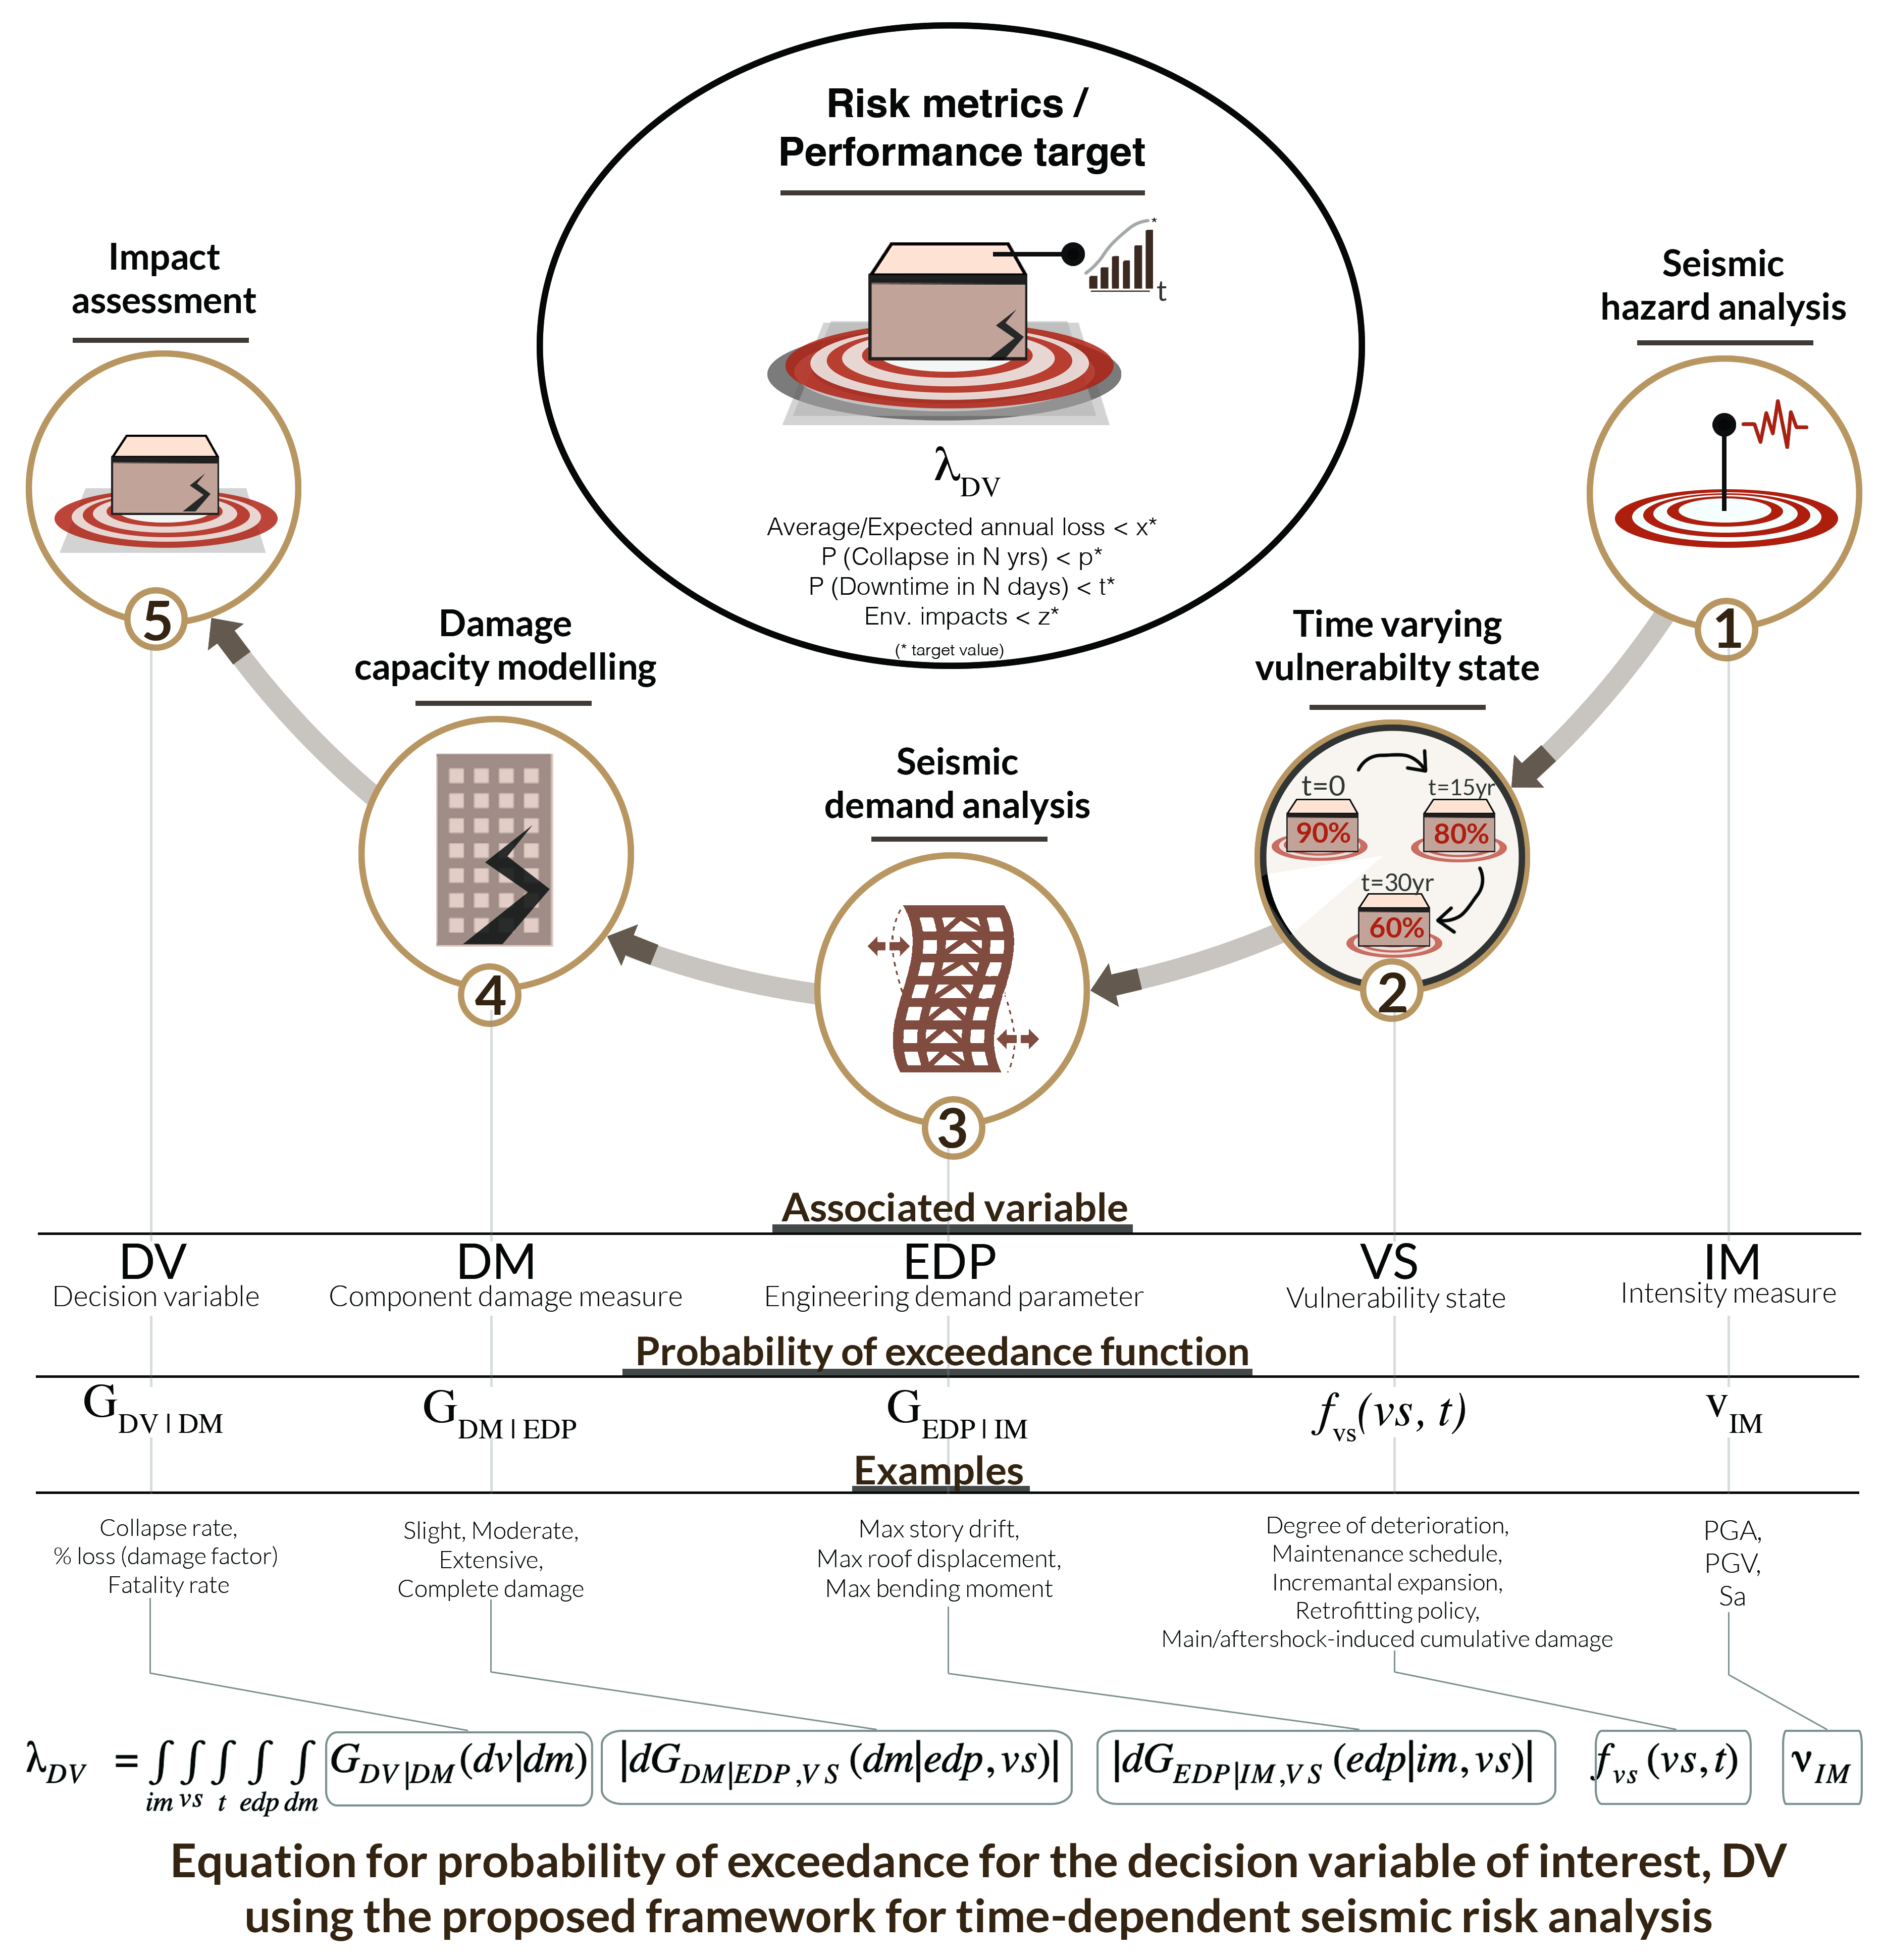
\includegraphics[width=\linewidth]{Figures/ICASP_Schematic1.jpg}
  \caption{Proposed framework accounting for time dependent vulnerability in seismic risk analysis}
  \label{fig:schematic1}
\end{figure*}  


\afterpage{%
    \clearpage% Flush earlier floats (otherwise order might not be correct)
    \begin{landscape}% Landscape page
\begin{figure*}[h!]
  \centering
  \includegraphics[width=\linewidth]{Figures/ICASP_Schematic2_matrix.jpg}
  \caption{Potential time-dependent vulnerability drivers for seismic risk and associated transition scenario}
  \label{fig:schematic2}
\end{figure*}  

\end{landscape}
\clearpage% Flush page
}

%% Discussion of transition

\subsection{Mathematical representation of vulnerability states and corresponding transition scenario}

Along with the proposed framework shown in Figure \ref{fig:schematic1}, we illustrate in Figure \ref{fig:schematic2} several potential time-dependent vulnerability drivers for seismic risk.

A certain vulnerability state can be dependent on the building's degree of deterioration, state of expansion, current structural condition, or the developed retrofit standard depending on the significant vulnerability drivers of interest to a certain structure. Given in Figure \ref{fig:schematic2} are suggested relative vulnerability states exhibiting increasing seismic vulnerability (for deterioration and building replacement) and decreasing vulnerability/increased resilience states (for seismic retrofitting).

Using Markov Chains is a simple approach to represent the transition of these discrete states over time. Markov chains are used to map the probability of transitioning from one state to another state in a specific time interval. Markov models are “memoryless”, such that the new state is solely dependent on the current state; not on the set of events preceding it \citep{agresti2003categorical}. The column showing the 'Transition Scenario' provides a schematic of the types of transition processes linked to each time-dependent vulnerability driver, and can then be mapped into corresponding transition probability matrices.

For instance, a non-retrofitted building can either transition into a retrofitted state with a certain probability within a year, or it can stay in its current state. Similarly, a building can also transition into a more deteriorated state over time with an associated transition probability. A common assumption for analysis incorporating structural deterioration or seismic retrofitting is that once a certain state is reached, it cannot go back to a previous state. For example, we assume that once a building is retrofitted, it is not possible for the building to go back to its unretrofitted state. In the schematic for the transition scenarios (Fig. \ref{fig:schematic2}) of deterioration and seismic retrofitting, this is shown by having all transition arrows going to the right only.
On the contrary, possible transition patterns for building replacements can bring back a building to its original (as-new) state as time goes by as presented by the arrows going to the left in its transition scenario diagram (Figure \ref{fig:schematic2}). Alternatively, a building could be replaced by another built to higher standards, as is often the case resulting from building code improvements. The same figure also shows a sample transition probability matrix for each vulnerability driver using the given time-dependent vulnerability states. The size of the transition probability matrix depends on the potential vulnerability states considered in the analysis, but they should exhibit similar pattern. 

Depending on the transition rates, $d_{i,i}$, $b_{i,i}$, $r_{i,i}$, the transition between the vulnerability states can go either slower or quicker based on different factors. For example, building deterioration rates are usually affected by the level of environmental exposure of the structure, its initial structural quality, or the implemented maintenance schedule which could potentially mitigate the seismic risk over time.
It should be noted that the factors affecting transition rates don't necessarily affect the actual fragility curve for each state.

Fragility curves define the state of vulnerability of a building or structure. These curves show the relationship of the earthquake intensity and the probability of exceeding a particular damage level.

Numerous methods exist to derive these curves: (1) analytical \citep{singhal1996method, lallemant2015statistical}, (2) empirical \citep{sanchez2005science,noh2015development} or heuristic/ based on expert opinion \citep{jaiswal2012use}.

Given a hazard curve at a study site, the annual collapse rate of a building is calculated by integrating the fragility curve over the hazard curve in Equation \ref{eq:onebldg}.
\begin{equation}
\begin{split}
    \lambda_{Collapse} = \Int_{IM_{min}}^{IM_{max}} P(Collapse |IM=im) | d\lambda_{im} (im) |
\end{split}
\label{eq:onebldg}
\end{equation}

where $\lambda_{im} (im)$ is the seismic hazard curve and $| d\lambda_{im} (im) |$ is the absolute value of the derivative of the hazard curve.

For a portfolio of buildings  the annual expected number of building collapse at a time $t$ can be calculated using Equation \ref{eq:port}.
%\begin{footnotesize}
%\begin{strip}
\begin{equation}
\begin{split}
    \lambda_{Collapse Total}(t) = \sum_{State_{1}}^{State_{n}}\Int_{IM_{min}}^{IM_{max}}\\
     P(Collapse |IM=im)| State=State_{i})  \\
     \times \; P(State=State_{i} |D_{o} =d_{o}, P=p)(t) \\
    \times \; | d\lambda_{IM} (im) |
\end{split}
\label{eq:port}
\end{equation}
%%\end{footnotesize}

where $P(Collapse |IM=im)| State=State_{i}$ is the fragility curve for each building state at collapse,  
$P(State=State_{i} |D_{o} =d_{o}, P=p)(t)$  is the probability of being in a building state at time $t$ for a given transition probability matrix $p$ and initial state distribution $d_{o}$.

It can be shown that the expected vulnerability state distribution $D_t$ at time $t$ is $E(D_t|D_o=d_o) = d_oP^t$ where $P$ is the transition probability matrix of vulnerability states. Therefore \ref{eq:port} can be re-written as:
\begin{equation}
\begin{split}
    \lambda_{Collapse Total}(t) = \sum_{State_{1}}^{State_{n}}\Int_{IM_{min}}^{IM_{max}}\\
    P(Collapse |IM=im)| State=State_{i}) \\
   \times \;  d_oP^t \; | d\lambda_{IM} (im) |
\end{split}
\label{eq:port2}
\end{equation}


\section{Case studies}

\subsection{Building-level deterioration analysis}

We apply the methodology discussed previously to model the changing risk of a hypothetical deteriorating building over time, we focus on three (3) vulnerability states ranging from as-new, heavily deteriorated and very heavily deteriorated for a hypothetical reinforced concrete (RC) building. 

A hypothetical vulnerability curve is generated to represent the non-deteriorated state. For simplicity, we only use fragility curves corresponding to "Extensive/ Complete Damage.”

Vulnerability curves for the three (3) assumed vulnerability states corresponding to each degree of deterioration,$w$, are obtained using Equations \ref{eq:rao1} and \ref{eq:rao2} \citep{rao2017development}. 
\begin{equation}
\begin{split}
    m(w) = m_{o}e^{-\alpha_{m}w}
\end{split}
\label{eq:rao1}
\end{equation}
\begin{equation}
\begin{split}
    \xi(w) = \xi_{o}(1-\alpha_{\xi}w)
\end{split}
\label{eq:rao2}
\end{equation}

where \\
$m(w)$, $\xi(w)$= median and dispersion of fragility function at level of deterioration $w$ consecutively ,\\
%$\xi(w)$= dispersion of the fragility function at a level of deterioration $w$, \\
$m_{o}$, $\xi_{o}$ = median and dispersion of the fragility function for the column in its non-corroded state consecutively\\
%$\xi_{o}$=  dispersion of the fragility function for the column in its non-corroded state, \\
$\alpha_{m}$=  exponential decrement function for the median and \\
$\alpha_{\xi}$=  coefficient of the linear decrement function for the dispersion of the fragility function.

The coefficients of the decrement function are adopted from estimates by \cite{rao2017development} for a hypothetical RC column built in 1960 to pre-1971 design standards: 
$m=1.43$,	$\alpha_{\xi}= -0.18 $

Using the framework for this application, we compare the impact of different levels of maintenance on seismic risk over time. Three maintenance schemes are used to demonstrate the diversity of maintenance options for seismic safety: (1) Low, (2) Medium, and (3) High Maintenance.
Transition probability matrices are assumed based on a Markovian model developed by Duling (2006) for an RC building constructed with pre-1971 design standards to predict the building service life given three varying levels of maintenance. The percent change in annual collapse risk normalized to baseline risk at t=0 is calculated using Equation \ref{eq:onebldg} and presented in Figure \ref{fig:bldglevel}. 

The trends shown in the figure highlight the impact of building deterioration on the seismic risk of buildings, and the benefits of maintenance; it demonstrates the importance of accounting for time-dependent vulnerability drivers such as deterioration in studying future seismic risk of a building. This demonstration shows that the proposed framework enables the testing of impact of maintenance or other building mitigation strategies on seismic risk over time. If linked with financial loss information, the framework could be used for cost benefit analysis for mitigation.

\begin{figure}[htbp!]
  \centering
  \includegraphics[width=\linewidth]{Figures/building_level.png}
  \caption{Percent change in annual collapse risk normalized to baseline risk at t=0 for a hypothetical building}
  \label{fig:bldglevel}
\end{figure}  

%%% DISCUSSION

%% Building levels
%% The framework demonstrates how we can investigate changing vulnerability over time driven by these factors
%% Buildings deteriorate over time even with high level of maintenance - this needs to be accounted for
%% It also enables to test impact maintenance or other building mitigation strategies
%% If linked with, financial loss, it could be used for cost benefit analysis for mitigation

%%%%%%%%%%%%%%%%%

\subsection{Policy analysis for community level seismic risk reduction}


%%%% Seismic Risk Reduction Policies


Using the proposed framework, we can also test the impact of various seismic risk reduction policies at a regional level. A hypothetical urban community was simulated, consisting of four districts each having their own building type distribution and seismic hazard curve. For simplicity of demonstration, the design of buildings are either high grade or low grade, and each can transition to deteriorated states, retrofitted states (for low-grade buildings), or get replaced over time. Hypothetical fragility curves are developed to represent each of these states: (1) Undeteriorated/unretrofitted state (2) Heavily deteriorated state (3) Very heavily deteriorated state (4) Retrofitted state with low standard and (5) Retrofitted state with high standard. The fragility curves for each vulnerability state are shown in figure \ref{fig:fragcurves}.

Hazard curves for each district are synthetically generated as idealized power-law hazard curves of the following form:
\begin{equation}
\begin{split}
    \lambda_{im} (IM) = k_{o}IM^{-k}
\end{split}
\label{eq:rao2}
\end{equation}

Parameters used for the four districts are k0 = 0.0002, 0.0003, 0.00022, 0.00035 and k = 2, 2.1, 2.2, 2.5
for districts 1, 2, 3 and 4 respectively.

%%Maybe insert plot of fragility curves

\begin{figure}[htbp!]
 \centering
  \includegraphics[width=.7\linewidth]{Figures/fragcurves5.jpg}
  \caption{Fragility curves for assumed vulnerability states at the hypothetical building stock}
  \label{fig:fragcurves}
\end{figure} 

% Please add the following required packages to your document preamble:
% \usepackage{booktabs}


\begin{table}[]
\centering
\caption{Indices of Transition Probability Matrices. (Abbreviations: HD = Heavily deteriorated, VHD = Very heavily deteriorated, n/a = Unretrofitted building}
\begin{tabular}{@{}lllllllll@{}}
\toprule
Index                                                             & P1     & P2   & P3   & P4     & P5  & P6  & P7     & P8     \\ \midrule
\begin{tabular}[c]{@{}l@{}}Building\\ design grade\end{tabular}   & high   & high & high & low    & low & low & any    & any    \\ \midrule
\begin{tabular}[c]{@{}l@{}}Degree of\\ deterioration\end{tabular} & as-new & HD   & VHD  & as-new & HD  & VHD & as-new & as-new \\ \midrule
\begin{tabular}[c]{@{}l@{}}Retrofit\\ standard\end{tabular}       & n/a    & n/a  & n/a  & n/a    & n/a & n/a & low    & high   \\ \bottomrule
\end{tabular}
\label{tab:mat}
\end{table}


%\begin{figure}[htbp!]
 %\centering
 % \includegraphics[width=5cm]{Images/trans_format.jpg}
 % \caption{Form of transition probability matrix for the community level policy analysis. Refer to Table \ref{tab:mat} for description of each state.}
 % \label{fig:transformat}
%\end{figure} 

\begin{figure}[htbp!]
 \centering
  \includegraphics[width=.7\linewidth]{Figures/trans_low.jpg}
  \caption{Transition probability matrix calibrated for a low quality seismic risk reduction scheme described in Table \ref{tab:policylist}}
  \label{fig:transprob1}
\end{figure} 

\begin{figure}[htbp!]
 \centering
  \includegraphics[width=.7\linewidth]{Figures/trans_high.jpg}
  \caption{Transition probability matrix calibrated for a high quality seismic risk reduction scheme described in Table \ref{tab:policylist}}
  \label{fig:transprob2}
\end{figure} 



The purpose of the framework developed is to compare the impact of
various policies on seismic risk over time. The types of decisions in the policy-making space includes the level of retrofit standards used, maintenance schedule and rate of development (building replacement) in each district. All these are being implemented while taking into account deterioration rate. Mathematically, the transition matrix for this type of problem is represented by a combination of the typical transition probability matrices shown in Figure \ref{fig:schematic2}. Two community-level policies are simulated using the proposed framework as described in Table \ref{tab:policylist}. Corresponding transition probability matrices for each policy are shown in Figures \ref{fig:transprob1} and \ref{fig:transprob2}. Each value corresponds to the probability of each state described in Table \ref{tab:mat} to  transition to the next state.

\afterpage{%
    \clearpage% Flush earlier floats (otherwise order might not be correct)
    \begin{landscape}% Landscape page
% Please add the following required packages to your document preamble:
% \usepackage{booktabs}
% \begin{tiny}
\begin{table*}[]
\centering
% \footnotesize
\caption{Features of seismic reduction policies tested on a hypothetical community}
\begin{tabular}{@{}lll@{}}
\toprule
Policy feature              & Low quality seismic reduction scheme                        & High quality Seismic reduction scheme                         \\ \midrule
Retrofit policy             & Voluntary, long time frame, low standard & Mandatory, short time frame, high standard \\
Building replacement policy & Low rate of replacement                                     & High rate of replacement                                      \\
Maintenance schedule        & Low level maintenance schedule                              & High level maintenance schedule \\\bottomrule                             
\end{tabular}
\label{tab:policylist}
\end{table*}
% \end{tiny}
\end{landscape}
\clearpage% Flush page
}

Using Equation \ref{eq:port}, the change in risk linked to these two policies implemented on the hypothetical building stock is demonstrated in Figure \ref{fig:commlevel}. As expected, mandatory retrofit schemes with shorter time frames result in early and rapid reduction in seismic risk (Figure \ref{fig:commlevel}). Also, better maintenance schedules significantly slow down the deterioration of a building portfolio thus reducing seismic risk over time. Demonstrated in the hypothetical building stock case as well is that encouraging development or high building replacement rates to better code standards contributes to seismic risk reduction over time. This demonstration of a policy analysis for community level seismic risk reduction demonstrates the capability of the proposed framework to compare various policy choices related to different standard of improvements such as building codes or time frame for which these policies are enforced/implemented.

Note that the framework can be used to test complex combinations of policies, including encouraging development in lower-hazard districts, different retrofit time-frames, retrofit standards, new building codes, and much more.

\begin{figure}[htbp!]
  \centering
  \includegraphics[width=\linewidth]{Figures/community_level.png}
  \caption{Percent change in annual collapse risk normalized to baseline risk at t=0 for a hypothetical building stock. Refer to Table \ref{tab:policylist} for descriptions of each policy }
  \label{fig:commlevel}
\end{figure} 

% Community level
%%% Add another policy (middle curve?)
%% Demonstrates time dependent risk community scale driven by all these facotrs
%enables comparison of various ppolicy choices both related to standard of imprpovemnets - building codes, time frame for which policies are enforced/implemented


\section{Conclusion}

This paper presents a flexible framework accounting for time dependent vulnerability in seismic risk analysis. 
This enables modelling both of those processes that increase vulnerability (e.g.deterioration, building expansions, cumulative damage), those policies that mitigate increase in vulnerability (e.g. better maintenance schedule, higher durability construction) and those policies that improve resilience (e.g. seismic retrofits and building replacement to higher standards).

We provided multiple applications of the proposed framework for risk analysis that accounts for time-dependent vulnerability. We demonstrated a building-level deterioration analysis and a community-level seismic risk reduction policy analysis. The applications vary in terms of the modelled drivers of changing vulnerability and the scale of application (building-level vs. community-scale). In Appendix \ref{app-time-paper}, I include a short paper that demonstrates a variation of the flexible community-scale analysis shown in this chapter. The application focuses on testing seismic retrofitting programs with varying levels of retrofit standard, time-frame of implementation and whether the program is mandatory or voluntary. The case study in Appendix \ref{app-time-paper} uses fragility data and transition probabilities derived from New Zealand's seismic retrofit implementation records. This example further highlights the potential and flexibility of the time-dependent risk framework presented in this chapter to evaluate specific risk interventions.

Overall, the methodology builds on the fundamental probabilistic performance based framework by adding a component for time-varying features which affect vulnerability. The framework allows stakeholders to study the consequences of different mitigation schemes to future seismic risk, and analyse its sensitivity to the initial building stock quality, the structural deterioration rate, maintenance schedule, features of mandatory retrofit policies in terms of their time-frame and standard, building replacement rate, urban development rates and pattern, and other drivers of changing risk.


%----------------
\section{Acknowledgments}
%----------------
This research is funded through a National Research Foundation (Singapore) Fellowship grant (NRF–NRFF2018–06), along with an Earth Observatory of Singapore scholarship.


%The current demonstration is simplified.. 
% LImitattion

%%% Change module --> component
%% 

     \setcounter{chapter}{3}
\chapter[Learning from successes, not catastrophe: Using counterfactual analysis to highlight successful disaster risk reduction intervention]{Learning from successes, not catastrophe: Using counterfactual analysis to highlight successful disaster risk reduction intervention}\label{chap-counterfactual}

\begin{small}
\\
Chapter 4 is a journal article published as follows. Appendix \ref{app-pls-1} pertains to the Supplementary Material published with the paper.
\\ \\
\noindent
    \textbf{Rabonza M.L.}, Lin Y.C. and Lallemant D. (2022) Learning From Success, Not Catastrophe: Using Counterfactual Analysis to Highlight Successful Disaster Risk Reduction Interventions. \textit{Front. Earth Sci.} 10:847196. doi: 10.3389/feart.2022.847196
\\
\\
In addition, this chapter cites the following first-author paper, which is included in Appendix \ref{app-pls-2}. The paper presents the concept of four situations in which disaster risk reduction interventions go un-noticed. Two out of the four situations are addressed in Chapter 4's case studies.
\\
\\
\noindent
\textbf{Rabonza, M.L.}, Lallemant,  D.,  Lin,  Y. C., Tadepalli,  S., Wagenaar,  D., Nguyen,  M., Choong,  J., Liu,  C. J. N., Sarica,  G. M., Widawati,  B. A. M., Balbi,  M., Khan,  F., Loos,  S. \& Lim,  T. N. (2022). Shedding light on avoided disasters : measuring the invisible benefits of disaster risk management using probabilistic counterfactual analysis. \textit{A contributing paper to the United Nations Office for Disaster Risk Reduction (UNDRR) Global Assessment Report 2022}. https://www.undrr.org/publication/shedding-light-avoided-disasters-measuring-invisible-benefits-disaster-risk-reduction

% \label{app-pls-1}

%----------------
% \section*{Highlights}
% %--- RESEARCH HIGHLIGHTS
% %----------------
% \begin{itemize}

% \item I combine probabilistic risk analysis and counterfactual analysis to quantify and highlight the benefits of risk reduction that often go unnoticed.

% \item I estimate the benefits of an intervention in a past earthquake, and for a hazard that has not yet occurred.

% \item I highlight the success of the seismic retrofitting program for schools in Nepal during the 2015 Gorkha earthquake, and the benefits of scaling up the program.

% \end{itemize}


%%% Start of highlights
\clearpage
\vspace*{\fill}
\begingroup
\centering

\textbf{\Large{Chapter highlights}}

\hrulefill 

\begin{itemize}
\item \textsl{I combine probabilistic risk analysis and counterfactual analysis to quantify and highlight the benefits of risk reduction that often go unnoticed.}

\item \textsl{I estimate the benefits of an intervention in a past earthquake, and for a hazard that has not yet occurred.}

\item \textsl{I highlight the success of the seismic retrofitting program for schools in Nepal during the 2015 Gorkha earthquake, and the benefits of scaling up the program.}
\end{itemize}


\endgroup
\vspace*{\fill}


% %----------------
% \vspace{2cm}
% \noindent
% \textbf{Keywords:} Counterfactual analysis, Probabilistic risk, Disaster risk reduction, Risk framework, School earthquake safety

\end{small}
\clearpage



%%%%%%%%%%%%%%%%%
\section{Abstract}

In the aftermath of a disaster, news and research attention is focused almost entirely on catastrophic narratives and the various drivers that may have led to the disaster. Learning from failure is essential to preventing future disasters. However, hyperfixation on the catastrophe obscures potential successes at the local scale, which could serve as important examples and learning resources in effective risk mitigation. To highlight effective risk mitigation actions that would otherwise remain unnoticed, we propose the use of probabilistic downward counterfactual analysis. This approach uses counterfactual modelling of a past hazard event with consequences made worse (i.e. downward counterfactual) by the absence of the mitigation intervention. The approach follows probabilistic risk analysis procedures where uncertainties in the simulated events and outcomes are accounted for and propagated. We demonstrate the method using a case study of Nepal’s School Earthquake Safety Program, implemented before the 2015 $M_{w}$ 7.8 Gorkha earthquake. Using a school building database for Kathmandu Valley, Nepal, we present two applications: (1) the quantification of lives saved during the Gorkha earthquake as a result of the retrofitting of schools in Kathmandu Valley since 1999, (2) the quantification of the annual expected lives saved if the pilot retrofitting program was extended to all school buildings in Kathmandu Valley based on a probabilistic seismic hazard model. The shift in focus from realised outcome to counterfactual alternative enables the quantification of the benefits of risk reduction programs amidst disaster, or for a hazard that has yet to unfold. Such quantified counterfactual analysis can be used to celebrate successful risk reduction interventions, providing important positive reinforcement to decision-makers with political bravery to commit to the implementation of effective measures.


%%%%%%%%%%%%%%%%%%%%%%%%%%%%|
%%% INTRODUCTION
%%%%%%%%%%%%%%%%%%%%%%%%%%%%|
\section{Introduction}
\label{section-intro}

Success in disaster risk management (DRM) means that natural hazard events do not turn into disasters, and communities continue to function and be resilient to shocks and stresses from hazards. Since the extent of a disaster can be characterised by loss of life and disruptions to the physical, built and social environments, \citep{mileti1999disasters, smith2005through, moore1958tornadoes}, the extent of success of risk reduction interventions manifest primarily as reduced impact. As such, success is measured as an \textit{absence} (e.g. no damage, fewer casualties, etc). This poses a challenge for recognising and incentivising important investments in DRM interventions since they are made invisible by their very nature.

In the aftermath of earthquakes, storms, and floods, narratives of catastrophe dominate the interest of media, political and research communities. However, this hyper-fixation on the catastrophe can obscure important successes amid the broader disaster. Another challenge is to recognize successful interventions if the hazard they were designed for has not yet occurred. This happens when we rely on a disaster occurrence to make mitigation benefits visible. For extreme and rare hazard events, for example, the benefits of risk reduction may manifest only in the distant future. Because of the significant time delay between the interventions and their benefits being manifested, such interventions can be perceived as unsuccessful or squandered until the event occurs. These are two of the challenges described in \cite{lallemant_rabonza_gar_2022} where successful DRM interventions are made invisible: \textit{invisible success in the midst of broader disaster}, and \textit{invisible success due to yet unrealised benefits} (Full paper included as Supplementary in the Appendix). These \textit{invisible successes} of mitigation interventions are related to a cognitive tendency called \textit{outcome bias} - the tendency to judge the quality of a decision by the outcome alone \citep{robson_2019}. 

To address outcome bias, we propose a \textit{probabilistic downward counterfactual analysis} approach. It relies on comparing the outcome of a realised event in which a risk reduction was implemented, to an alternative branch of history (i.e. \textit{counterfactual}) in which the disaster risk reduction intervention was not implemented.  Throughout the paper, we use the term \textit{realised}  to refer to events or outcomes that transpired (in juxtaposition to counterfactual), in alignment with prior literature on probability and counterfactual analysis \citep{roese1997counterfactual}.  An imagined scenario where an intervention is absent is considered a \textit{downward counterfactual} because the assumed outcome is worse than what was observed in reality \citep{roese1997counterfactual}.  This is in contrast with an \textit{upward counterfactual} where the assumed outcome is better. Probabilistic downward counterfactual analysis is \textit{probabilistic} in that it follows probabilistic risk analysis procedures to propagate and account for uncertainties in events and outcomes. In this paper, we present two applications of probabilistic downward counterfactual analysis to highlight the effectiveness of risk reduction in terms of probabilistic lives saved. The first application estimates the benefits of an intervention in a past earthquake through comparison of fatalities modelled without the risk intervention and actual fatalities. The second application estimates the probabilistic benefits of a mitigation for a hazard that has not yet occurred. Instead of an actual past event, a hazard model is used to calculate the intervention's benefits.

The paper’s main contribution is in combining the probabilistic risk analysis framework and counterfactual analysis to calculate and highlight lives saved from successful disaster risk reduction interventions, that otherwise go unnoticed. The significance and novelty of this work is in shifting our perception of the benefits of risk reduction intervention, by using an appropriate counterfactual scenario as the baseline against which to calculate and judge these benefits. Rather than focusing entirely on realised outcomes, the analysis of counterfactual outcomes shines light on the value of a mitigation intervention by demonstrating what would have been without such intervention. Downward counterfactual risk analysis has only so far been used to identify potential worse impacts for the purpose of insurance, preparedness, or future mitigation \citep[e.g.][]{lin2020modeling, aspinall2019counterfactual, woo2019downward, woo2018counterfactual, shepherd2018storylines, woo2017reimagining, oughton2019stochastic, aspinall2019counterfactual}. This study pioneers a systematic approach to creating incentives for good decision-making on the basis of probabilistic risk. The quantification of probabilistic lives saved by effective risk reduction programs in a major hazard event serves as a powerful indicator of the intervention's success that would otherwise remain unnoticed amidst a disaster. In addition, the calculated probabilistic benefits of an intervention provide important incentive and encouragement to decision-makers committed to implementing effective measures even if the benefits are not materialized yet by the occurrence of a hazard event. Altogether, this work is a new domain of application of counterfactual analysis with much potential across the broad spectrum of hazards. 

The proposed framework has significant implications to multiple potential stakeholders. For policymakers, there is currently little political capital gained from investing in resilience if the benefits of such investments are invisible. By having the benefits of these investments visible to their constituents, policymakers will be incentivised for risk-informed decision-making. For donors and funders, this framework would enable them to monitor progress in terms of probabilistic impacts reduced, even if such benefits remain unrealized until a disaster strikes. For disaster risk management practitioners, while it is important to learn from failures, it is equally important to learn from successes, and share them broadly so they can be emulated, scaled, and adapted in other contexts where they are needed. Importantly, it also provides a mechanism to recognise and elevate the important, humble, long-term, and dedicated work conducted by many to keep our communities safe, even when their work is unseen.

The paper is organized as follows. Section \ref{section-counter} introduces the proposed framework in the context of probabilistic risk analysis. In Section \ref{section-retrofit-program}, we describe the earthquake risk intervention that will be the focus of our two applications: the school earthquake retrofitting program in Nepal, implemented before the 2015 $M_{w}$ 7.8 Gorkha earthquake. In the subsequent sections, we present the methods (Section \ref{section-methods}) and two applications (Section \ref{section-apps}) that shed light on the benefits of the retrofitting program. The first application estimates the number of lives saved during the Gorkha earthquake as a result of the retrofitting of schools in Kathmandu Valley since 1997. The second application calculates the annual expected lives saved if the retrofitting program was extended to all school buildings based on a probabilistic seismic hazard model we generated for Kathmandu Valley, Nepal. This is followed by Discussion (Section \ref{section-discussion}) and Conclusion (Section \ref{section-conclusion}).


%%%%%%%%%%%%%%%%%%%%%%%%%%%%|%%%%%%%%%%%%%%%%%%%%%%%%%%%%|
%%% COUNTERFACTUAL ANALYSIS
%%%%%%%%%%%%%%%%%%%%%%%%%%%%|%%%%%%%%%%%%%%%%%%%%%%%%%%%%|
\section{Counterfactual risk analysis framework}
\label{section-counter}

The main idea of counterfactual disaster risk analysis is to explore alternative branches of history to assess past situations where a disaster might have occurred but was averted or failed to materialise \citep{woo2018counterfactualvar}. Impacts associated with a past event, i.e. a realised event, can be expressed as the function of the (a) Hazard, the likelihood of potentially damaging events, (b) Exposure, the characteristics of assets such as people, buildings and infrastructure and (c) Vulnerability, the susceptibility of the exposed assets to sustain impact for a given hazard intensity \citep{UNISDRterms2009}. Then, we can write the losses from the realised event as 

\begin{equation}\label{eq:realised}
        I_{realised} = f \left( \theta_H, \theta_E, \theta_V \right),
    \end{equation}
where $\theta_H$, $\theta_E$, and $\theta_V$ are the hazard, exposure and vulnerability parameters consecutively. Modifications ($\delta_.$) of one or multiple parameters that define the realised event allow one to define the impact of a counterfactual event:

\begin{equation}\label{eq:counterfactual_risk}
    I_{counterfactual} = f \left( \theta_H + \delta_H,  \theta_E + \delta_E,  \theta_V + \delta_V \right),
    \end{equation}

The purpose of the deviations, $\delta_H$, $\delta_E$, and $\delta_V$, to the realised event’s parameters is to explore counterfactuals. $\delta_H$ helps us explore counterfactuals in the hazard (e.g. what if the earthquake had occurred at a slightly different location, or with opposite directivity of rupture?). $\delta_E$ helps us explore counterfactuals in the exposure (e.g. what if the 1906 San Francisco earthquake were to hit today’s building stock?). $\delta_V$ helps us explore counterfactuals in vulnerability (e.g. what if all unreinforced masonry buildings had been retrofitted?). In this paper, we focus on $\delta_V$, while $\delta_H$ and $\delta_E=0$, to highlight the value of effective vulnerability reduction programs that often go unnoticed.

Modelling the impact of events with either Equation \ref{eq:realised} or \ref{eq:counterfactual_risk} relies on probabilistic risk analysis. Traditionally used in engineering reliability assessments and performance-based design, probabilistic risk analysis has been an established approach to assess the risks from natural hazards to entire regions and cities \citep{pate2002risk, stergiou2010risk}. Probabilistic risk analysis systemically quantifies the potential impacts of hazard events on a system and the likelihood that such consequences would occur \citep{bedford2001probabilistic}. In the case of Equations 1 and 2, the impacts $I_{realised}$ and $I_{counterfactual}$ and their likelihood are obtained through the joint probability of the risk parameters.

The expected benefits ($B$) of effective risk mitigation is then calculated as the difference between the expected value (the mean) of impacts of the realised event $E(I_{realised})$ and the counterfactual event $E(I_{counterfactual})$ (see Equation \ref{eq:benefits} and Figure \ref{fig:conceptual_diagram}). Assuming the realised impacts are less than those of the counterfactual, $B$ is expected to be a positive value in Equation \ref{eq:benefits}.
    \begin{equation} \label{eq:benefits}
        B = E(I_{counterfactual}) - E(I_{realised})
    \end{equation}


\begin{figure}[h!] 
\begin{center}
    \includegraphics[width=\textwidth]{Figures/concept-diagram_rev2.png}
    \caption{The concept of the counterfactual risk analysis framework for quantifying the probabilistic benefits of effective risk reduction. This graphic serves as a demonstration of the framework that is specific for a risk intervention that reduces vulnerability.}
    \label{fig:conceptual_diagram}
\end{center}
\end{figure}

%%%%%%%%%%%%%%%%%%%%%%%%%%%%|%%%%%%%%%%%%%%%%%%%%%%%%%%%%|
%%% SCHOOLS RETROFIT
%%%%%%%%%%%%%%%%%%%%%%%%%%%%|%%%%%%%%%%%%%%%%%%%%%%%%%%%%|
\section{Invisible success of seismically retrofitting schools in Nepal}
\label{section-retrofit-program}

In this paper, we implement the proposed framework to highlight invisible benefits of effective earthquake risk mitigation. Specifically, we focus on one of the most significant risk interventions in recent years that led to improved construction practices - the seismic retrofitting of school buildings in Nepal. Amid the destruction and tragic loss during the Gorkha earthquake, the life-saving benefit of the school retrofitting was obscured. Likewise if an earthquake event has not yet occurred, retrofitting program may seem like a waste even though an earthquake may occur at any time. Probabilistic counterfactual risk analysis can be used to shed light on these invisible benefits.

School buildings in Nepal are recognized to be at high risk amidst the region's high seismicity from the convergence of the Indian tectonic plate with the Eurasian plate, and due to informal construction practices done with little engineering guidance \citep{marasini2020}. Damage to school buildings was extensive from large earthquakes in recent history - the 1988 $M_{w}$ 6.6 Udayapur earthquake \citep{gupta1988report}, and the 2011 $M_{w}$ 6.9 Sikkim/Nepal border earthquake \citep{rai2012reconnaissance}. The 2015 Gorkha earthquake is a unique example in terms of the impacts on schools because the earthquake happened on a Saturday, whilst the school was not in session. Had the earthquake hit on a school day, over one million students would have been affected \citep{dixit2014public}.

Seismic retrofitting of school buildings started in 1997 through the leadership of the National Society for Earthquake Technology (NSET) as part of Nepal's School Earthquake Safety Program (SESP)  \citep{marasini_2019}. By the time of the Gorkha earthquake in 2015, 300 schools had been retrofitted, 160 of which were in Kathmandu Valley. It was a big achievement that none of the schools retrofitted under SESP collapsed or needed major repairs after the earthquake. Because the buildings were found to be structurally sound, all the retrofitted buildings served as safe shelters and required fewer temporary classrooms \citep{marasini_2019}. 
Following the direction of SESP towards safe learning facilities, the Government of Nepal aims to achieve minimum school safety criteria nationwide by 2030 through the Comprehensive School Safety Master Plan developed by Nepal's Ministry of Education, Science and Technology \citep{cehrdc2018} based on the global Comprehensive School Safety Framework \citep{unisdr2017}. Recognizing the need to strengthen more than 60,000 school buildings all over Nepal \citep{marasini2020}, one of the activities in the Master Plan is to retrofit school buildings in earthquake-affected areas.

%%%%%%%%%%%%%%%%%%%%%%%%%%%%|%%%%%%%%%%%%%%%%%%%%%%%%%%%%|
%%% METHODS
%%%%%%%%%%%%%%%%%%%%%%%%%%%%|%%%%%%%%%%%%%%%%%%%%%%%%%%%%|
\section{Methods}
\label{section-methods}

\subsection{School building database}
% reference to a map?
The analyses in this paper are carried out on a database of Nepalese school buildings surveyed and georeferenced in 2013 through the partnership of the Open Data for Resilience Initiative (OpenDRI) and the Government of Nepal with support from Kathmandu Living Labs \citep{opendri_2012}. The building database covers Kathmandu Valley and was produced to understand the seismic risk in the education and health infrastructure. Parts in the dataset related to educational infrastructure were tagged as either \textit{school}, \textit{college}, \textit{university}, or \textit{kindergarten}. The database provides information on the location, number of daytime occupants on a school day, structure type, and whether the school building was retrofitted or not. We chose the OpenDRI dataset for this paper because these building attributes allow us to determine which school buildings were retrofitted under SESP before the 2015 Gorkha earthquake. In addition, the buildings’ structure type can be used to identify the buildings’ vulnerability, while the number of daytime occupants can be used for fatality calculations.

After screening the raw OpenDRI dataset for missing information or non-school buildings, the final dataset we use for this work consists of 5029 school buildings, of which 70 were retrofitted (see Figure \ref{fig:data-all}). We highlight that the OpenDRI dataset we use for this study provides information on only 70 out of the 160 retrofitted school buildings identified by NSET in Kathmandu Valley's affected areas \citep{marasini_2019}. The database consists of buildings with unreinforced masonry-type (URM-type) and reinforced concrete-type (RC-type) structures. The daytime occupancy for the 70 retrofitted schools go up to 800, with a mean of 134, whereas the occupancy for the 5029 school buildings go up to 2000 with a mean of 120.

\begin{figure}[h!] 
\begin{center}
    \includegraphics[width=\linewidth]{Figures/Datasets-basic.png}
	\caption{A map of the building database used in the analysis showing distribution of schools retrofitted and non-retrofitted as well as structure type.}
	\label{fig:data-all}
\end{center}
\end{figure}


\subsection{Building vulnerability modelling}
\label{section-vuln}

A fundamental step in estimating the benefit of a seismic retrofitting intervention involves obtaining the structure’s probability to exceed a certain damage level before and after the intervention. This paper focuses only on the collapse damage level since a vast majority of earthquake fatalities worldwide are due to building collapse \citep{spence2007saving}. Collapse fragility curves are used to represent the probability of collapse for a given earthquake intensity and building class. 

In this work, we have adopted collapse fragility curves developed by other authors to represent the probability of collapse of the buildings in their retrofitted and non-retrofitted states. The collapse fragility curves we use for the Nepalese school building stock in this study are presented in Figure \ref{fig:frag_curves}. The median $\eta$ and lognormal standard deviation $\beta$ of the fragility curves expressed as PGA lognormal distributions are shown in Table \ref{tab:frag_params}.

\begin{figure}[h!]
\begin{center}
    \includegraphics[width=\linewidth]{Figures/data-fragility-v4.png}
    \caption{Collapse fragility curves adopted in the analysis.}
    \label{fig:frag_curves}
\end{center}
\end{figure}

For non-retrofitted buildings, we adopt \cite{giordano2021empirical}'s empirical-based fragility curves specifically developed for Nepalese school buildings. The curves were generated using a Bayesian approach to incorporate well-established fragility models such as the HAZUS database \citep{mh20152} and World Bank's Structural Integrity and Damage Assessment database (SIDA) that was conducted under the Global Program for Safer Schools \citep{wbglosi}. The collapse fragility curves from \cite{giordano2021empirical} were assigned to the buildings in the OpenDRI dataset based on their structure type - unreinforced load-bearing wall schools were assigned the URM collapse fragility curve, while reinforced concrete schools were assigned the RC collapse fragility.

% Percent of URM and RC for total
% Insert assignment of building classes

For retrofitted buildings, we use the collapse fragility curve developed by \cite{giordano2021financial} for retrofitted stone masonry buildings in Nepal that are considered to have good quality material. The fragility curves in \cite{giordano2021financial} were produced analytically using a non-linear static pushover analysis for stone masonry buildings retrofitted with the 'RC strong-back approach'. It should be noted that the selected fragility curve for retrofitted school buildings does not necessarily represent the variation in the retrofit solutions available in Nepal, as well as the workmanship and original quality of the buildings, rather this is the best information available to the authors at the time of writing.

\begin{table}[]
\caption{Fragility curve parameters adopted in the analysis for the school buildings in the OpenDRI database. The parameters follow a lognormal model where $\eta$ (g) is the median PGA and $\beta$ is the lognormal standard deviation.}
\label{tab:frag_params}
\resizebox{\textwidth}{!}{%
\begin{tabular}{|c|l|c|c|c|}
\hline
    \multirow{2}{*}{\begin{tabular}[c]{@{}c@{}}Reference\end{tabular}} &
    \multicolumn{1}{c|}{\multirow{2}{*}{Building class}} &
    \multirow{2}{*}{\begin{tabular}[c]{@{}c@{}}Structural state \\ of building\end{tabular}} &
    \multicolumn{2}{c|}{\begin{tabular}[c]{@{}c@{}}Collapse state \\ parameters\end{tabular}} \\ \cline{4-5} 
        & \multicolumn{1}{c|}{}   &   & $\eta$  & $\beta$  \\ \hline
    \rule{0pt}{3ex}%  EXTRA vertical height  
            
    \citep{giordano2021empirical} &
    \begin{tabular}[c]{@{}l@{}}Non-retrofitted URM - Unreinforced masonry bearing wall,\\ low-rise (pre-code)\end{tabular} &
        Un-retrofitted &
        0.55 &
        0.76 \\ \hline
    \rule{0pt}{3ex}%  EXTRA vertical height  
            
    \citep{giordano2021empirical} &
    \begin{tabular}[c]{@{}l@{}}Non-retrofitted RC - Concrete frame buildings with\\ unreinforced masonry infill walls, low-rise (low code)\end{tabular} &
        Un-retrofitted &
        1.13 &
        0.84 \\ \hline
    \rule{0pt}{3ex}%  EXTRA vertical height    
            
    \citep{giordano2021financial} & Retrofitted stone masonry buildings      & Retrofitted    & 1.133 & 0.452 \\ \hline

\end{tabular}%
}
\end{table}            


\vspace{0.5cm} % because the paragraph space seems to small here

\subsection{Expected fatalities from building collapse}

A vast majority of earthquake fatalities worldwide are due to building collapse \citep{spence2007saving}. Therefore, this paper focuses on quantifying the fatalities from earthquake-induced building collapse, and the reduced estimated fatalities from retrofitting interventions.

To estimate fatalities due to building collapse, we adopt a semi-empirical casualty model that takes advantage of the availability of detailed building inventory and collapse fragility curves specific to the building types in Nepal. The approach is adopted from the semi-empirical forward model implemented in the USGS Prompt Assessment of Global Earthquakes for Response (PAGER) system \citep{jaiswal2011earthquake} for determining the extent of earthquake impacts globally. In contrast to USGS PAGER's use of Modified Mercalli shaking intensities, the earthquake intensity for this study is expressed in terms of peak ground accelerations. In this study, we calculate the total estimated fatalities $E[I]$ for a given building portfolio having a total number of $m$ buildings from a single earthquake event. Each building $i$ in the portfolio has a known structure type $k_{i}$. Using the empirical casualty model, we can write $E[I]$ as

    \begin{equation}\label{eq:loss_fat}
    E[I] = \sum_{i=1}^{m} O_{i} \cdot FR_{i}(k_{i}) \cdot C_{i}(im_{i}, k_{i})
    \end{equation} 
    %% per event based on stochastic 

where $O_{i}$ is the total exposed population inside building $i$ at the time of the earthquake, $FR_{i}(k_{i})$ is the fatality rate associated with the collapse of building $i$ based on its structure type $k_{i}$, and $C_{i}(im_{i}, k_{i})$ is the probability of collapse of building $i$ given the earthquake intensity at its location $im_{i}$ and its structure type $k_{i}$.

A fixed fatality rate of $FR_{i}(k_{i}) = 20\%$ for all structure types $k_{i}$ in the dataset is adopted for the study. This fatality rate is based on NSET's recommendation for both RC and masonry building classes, of which all the buildings in the dataset fall into \citep{nset2000}. This comes with an assumption that the same level of casualty is expected regardless of the level of school (e.g. primary or higher grades), nature of escape routes, or the occupants' level of preparedness.

By calculating $E[I]$ for a counterfactual and a realised scenario using Equation \ref{eq:loss_fat}, and plugging into Equation \ref{eq:benefits}, we can calculate the expected benefits of effective risk mitigation in terms of lives saved. In order to generate the entire probability distribution of fatalities, we conduct Bernoulli simulations (10,000) for collapse given a shaking intensity $C_{i}(im_{i})$ at each building location and for each building class $k_{i}$ for both the realised and counterfactual scenario. The complete source code is available at https://github.com/ntu-dasl-sg/frontiers2021-PLS.

 
%%%%%%%%%%%%%%%%%%%%%%%%%%%%|%%%%%%%%%%%%%%%%%%%%%%%%%%%%|
%%% APPLICATIONS
%%%%%%%%%%%%%%%%%%%%%%%%%%%%|%%%%%%%%%%%%%%%%%%%%%%%%%%%%|
\section{Applications}
\label{section-apps}

\subsection{Lives saved during the 2015 Gorkha earthquake due to the school retrofitting in Kathmandu Valley}
\label{section-case1}

In order to quantify the reduced fatalities from the school retrofit program in Kathmandu Valley, we estimate the fatalities during the 2015 Gorkha earthquake in the 70 retrofitted school buildings in our database as well as in the counterfactual scenario where these are not retrofitted. By chance, the earthquake occurred during a school holiday, during which occupancy was very low. For both re-analysis scenarios (current retrofit and counterfactual non-retrofit schools), we analyse fatalities for the expected occupancy during the school day. While there were a total of 160 schools retrofitted in  Kathmandu Valley at the time of the 2015 Gorkha earthquake \citep{marasini_2019}, our database contained information on 70. Hence while the focus of our analysis is on the life-saving benefit of the retrofit of the 70 schools in our data, the true reduction in fatalities due to the earthquake retrofitting program is much greater. A map of the 70 retrofitted school buildings used in this analysis is shown in  Figure \ref{fig:datacase1}.

\begin{figure}[h!] 
\begin{center}
    \includegraphics[width=\linewidth]{Figures/Dataset_Case1.png}
	\caption{A map of the 70 retrofitted schools and their corresponding structure type used in the analysis described in Section \ref{section-case1}. The basemap shows the hazard model developed by \cite{chen20192015} for the 2015 Gorkha earthquake in terms of peak ground acceleration (in g-units).}
	\label{fig:datacase1}
\end{center}
\end{figure}

The shaking intensity at the school sites during the 2015 Gorkha earthquake is obtained from the broadband ground-motion simulations produced by \cite{chen20192015} for the earthquake event. This hazard model was selected because the location of sources of the high-frequency energy (strong-motion generation areas) is a critical factor in explaining the relatively low damage phenomenon observed in Kathmandu Valley during the 2015 Gorkha earthquake \citep{gallovivc2016modeling, koketsu2016widespread}, aside from the effects of site conditions and rupture directivity \citep{dixit2015strong, rajaure2017characterizing, gallovivc2016modeling, koketsu2016widespread}. A map of the PGA values at the location of the retrofitted buildings is shown in Figure \ref{fig:datacase1}. With this hazard model, PGA values at the location of the retrofitted buildings range from 0.065 to 0.149 g, and come in a resolution of 0.0167 degrees, or around 1.85km.  More details about the PGA data are summarised in \cite{chen20192015} and its companion paper, \cite{wei20182015}.

In order to calculate the estimated impacts in a counterfactual scenario, $E[I]_{counterfactual}$, in which the SESP seismic retrofitting program was absent before the Gorkha earthquake, we use Equation \ref{eq:loss_fat} to estimate the total fatalities for the 70 buildings under this counterfactual scenario. The probability of collapse $C_{i}(im_{i}, k_{i})$ of any building $i$ is obtained from the fragility curve of the building at its \textit{non-retrofitted state} and the Gorkha earthquake event-specific PGA at the building's location $im_{i}$. The collapse fragility curves for the non-retrofitted state are assigned as described in Section \ref{section-vuln}, and the PGA values at the building locations are extracted from \cite{chen20192015}'s hazard model. Using these inputs in Equation \ref{eq:loss_fat} results to $E[I]_{counterfactual}$ = 25 fatalities.

The expected fatalities from the realised event $E[I]_{realised}$ can be calculated using the same approach, but using the collapse fragility curves corresponding to the \textit{retrofitted state} of the buildings as assigned in Section \ref{section-vuln}. This approach results in $E[I]_{realised}$ = 0 fatalities, which is the expected total number of fatalities in the realised scenario for the 70 buildings. By comparing the fatalities from the two scenarios as in Equation \ref{eq:benefits}, we estimate that the lives of approximately 25 school occupants were saved in Kathmandu by the retrofit of the 70 schools (see Figure \ref{fig:results_case1}).

\begin{figure}[h!] 
\begin{center} 
    \includegraphics[width=\linewidth]{Figures/results_case1-v2.png}
	\caption{Distribution of estimated fatalities from the 2015 $M_{w}$ 7.8 Gorkha earthquake based on earthquake intensity values from \cite{chen20192015}. Two scenarios are shown: the actual scenario where all 70 school buildings were retrofitted prior to the 2015 Gorkha earthquake, and a counterfactual scenario where the schools were not retrofitted. Our analysis show an estimated 25 lives in the 70 retrofitted schools.}
\label{fig:results_case1}
\end{center}
\end{figure}

In an attempt to explore the sensitivity of the casualty estimates to different hazard models for the 2015 Gorkha earthquake, we repeated the analysis using a PGA map from the USGS ShakeMap \citep{shakemap2015nepal, wald2007topographic}. While using \cite{chen20192015}'s hazard model results in 25 lives saved, using the USGS ShakeMap hazard model results in 68 lives saved (see Figure \ref{fig:supplementary_ShakeMap} in the Appendix).  The analysis using either model highlights the life-saving benefit of the school retrofitting program, but we believe that the fatality analysis using \cite{chen20192015}'s model is more accurate in terms of representing the shaking during the 2015 Gorkha earthquake. \cite{chen20192015}'s model better captures the amplification or attenuation of the seismic shaking as it accounts for the location of sources of the high-frequency energy (strong-motion generation areas), rupture directivity, and site conditions critical in understanding the relatively low damage phenomenon observed in Kathmandu Valley during the earthquake. 

\vspace{0.5cm} % because the paragraph space seems to small here

\subsection{Annual expected lives saved through scaling the retrofit programs to all schools in Kathmandu Valley}
\label{section-case2}

Part of the Comprehensive School Safety Master Plan is the ambition to scale earthquake retrofitting to all vulnerable schools \citep{cehrdc2018}. As such, we develop a second case study to better understand the life-saving impact of such a program. We assess expected fatalities if the 5029 schools in Kathmandu Valley were retrofitted, and if they remained in their current state. This analysis is conducted for the entire seismic hazard of Nepal, to better reflect the distribution of potential events to impact Kathmandu Valley.

A probabilistic seismic hazard analysis (PSHA) was developed for the school building sites based on twenty-three independent seismic source zones for Nepal identified by \cite{ram2013probabilistic} and adopted in \cite{chaulagain2015seismic}’s PSHA model. The ground motion prediction equation by \cite{chiou2014update} for active shallow crust regions is used within a logic tree for an event-based probabilistic seismic hazard calculation in the OpenQuake-engine \citep{silva2014development}. To reach statistical convergence, 100,000 stochastic event sets with a 1-year time interval were generated \citep{silva2016critical}. The result of the simulation is a large number of realisations of seismic events and corresponding shaking at the locations of the schools within a year. The resulting hazard curves for some selected schools in the database are shown in Figure \ref{fig:hazcurve}.

\begin{figure}[h!] 
\begin{center}
    \includegraphics[width=\linewidth]{Figures/hazcurves-v5.png}
	\caption{Hazard curves for three sample school building locations in the analysis.}
	\label{fig:hazcurve}
\end{center}
\end{figure}

For every event generated, the number of fatalities in the building portfolio due to collapse is estimated using Equation \ref{eq:loss_fat}. In the fatality calculation of each event, we incorporate the probability distribution of school building occupancy. In Nepal, schools are open and run 220 days a year, and each school day lasts for 6 hours \citep{nepal2009reform}. This means that out of the 8760 hours in a year, 1320 (15\%) are school hours in Nepal. To account for this, we simulate a large number of Bernoulli trials for each event that takes a 15\% probability of occurring during school hours. The resulting annual fatality exceedance probability curves for two different retrofitting scenarios are shown in Figure \ref{fig:losscurve}. The fatality calculation in this study assumes no uncertainty related to the time of the day during school hours. This means that the building occupancy is constant during school hours, whereas outside school hours, the building occupancy is 0.

\begin{figure}[h!] 
\begin{center}
    \includegraphics[width=\linewidth]{Figures/loss_curve_ALL_100k-annotate.png}
	\caption{Benefits of extending Nepal's school retrofit program to 5029 schools in the database in terms of the shift in the annual fatality exceedance curve.}
	\label{fig:losscurve}
\end{center}
\end{figure}

The average annual fatalities are obtained by integrating the integrating the annual fatality exceedance probability curve. For the scenario in which none of the 5029 school buildings is retrofitted, we estimate 13 average annual fatalities, whereas when the retrofitting program is extended to all buildings, we estimate an average of 1 annual fatality. In this probabilistic analysis, we calculate an average of 12 annual lives saved from scaling the retrofit program in all of Kathmandu Valley.
%%%%%%%%%%%%%%%%%%%%%%%%%%%%|%%%%%%%%%%%%%%%%%%%%%%%%%%%%|
%%% CONCLUSION
%%%%%%%%%%%%%%%%%%%%%%%%%%%%|%%%%%%%%%%%%%%%%%%%%%%%%%%%%|
\section{Discussion}
\label{section-discussion}

\subsection{A counterfactual analysis approach to celebrate effective risk reduction}

In a field focused on long-term resilience to rare (i.e. volatile) hazard events, perceptions of risk are biased by realised outcomes. The perception of \textit{no impacts} when in fact DRM work is successful can result in policymakers and society at large to undervalue the importance of proactive intervention. Shedding light on successes and \textit{what might have been}, not only recognizes the outstanding work of those working to reduce risk, but is also a crucial component of encouraging decision-makers to continue investments in measures that keep our communities safe. 

We highlight the need to celebrate the often invisible successes of disaster risk reduction interventions, in order to incentivise, better learn and replicate investments in such interventions. We further propose and demonstrate the use of a probabilistic counterfactual risk analysis framework to identify, quantify and highlight these invisible successes. The framework demonstrates that judgement of a risk reduction intervention should be based on a broad exploration of possible outcomes, not only on specific outcomes.

We demonstrated two applications of the probabilistic downward counterfactual risk analysis to (1) celebrate lives saved by a disaster risk reduction intervention (earthquake school retrofitting) amidst a past event (the 2015 Gorkha earthquake in Nepal), and (2) assess expected annual lives saved due to the intervention with the use of a probabilistic hazard model. The two applications show that even in the midst of a tragic disaster, or if a hazard event has not occurred yet, there are often successes in risk reduction intervention to celebrate. The counterfactual analysis showed that numerous expected fatalities were avoided during the Gorkha earthquake because of the government-led retrofitting of school buildings starting in 1997, and many more could be saved if the retrofit program were scaled to all schools in Kathmandu Valley. 

\vspace{0.5cm} % because the paragraph space seems to small here

\subsection{Lives saved as a risk reduction benefit metric}

In our demonstrations, the risk benefit of DRM intervention is measured in terms of a reduction in loss of life - the first target metric within the Sendai Framework For Disaster Risk Reduction \citep{united2015sendai}. A risk benefit metric in financial units can also be used, as with a typical cost-benefit analysis. However such analysis tends to highlight interventions that effectively protect high-value areas instead of high-vulnerability areas, which exacerbates inequities \citep{markhvida_quantification_2020, lallemant2020informatics}. 

More alternative risk reduction benefit metrics for this analysis include the number of displaced people, business downtime, damage to buildings and cultural heritage, psychological distress and more. For the Nepal case study, for example, the benefits of retrofitting go well beyond the reduced physical vulnerability of the buildings. Retrofitted schools served as immediate community shelters, field hospitals and relief centres. Classes in the retrofitted buildings were operated without fear, resulting in less demand for temporary classrooms \citep{marasini2020}. Loss avoidance is not the only invisible benefit of disaster mitigation, and the benefits of DRM interventions go beyond reduction of impact. Certain intervention designs can have co-benefits such as retrofit programs that improve the environmental comfort of classrooms, that serve as training platforms to local constructors who replicate the methods in other building constructions, or that are linked with student and teacher earthquake preparedness programs \citep{spence2021buildings}.

\vspace{0.5cm} % because the paragraph space seems to small here

\subsection{First order approach}

The analyses and estimates of lives saved presented are first order and serve as proof of concept of the counterfactual framework to highlight successes in DRM. Following are limitations that need to be noted for future work:

\begin{itemize}
    \item 
    The analysis did not account for fatalities from partially collapsed buildings. To account for this, one may use NSET's recommendation to use a 10\% fatality rate for heavily damaged buildings \citep{nset2000}
    \item
    The building portfolio dataset we use in the two case studies is only a subset of all the schools within the study area. The dataset used for the first case study (Section \ref{section-case1}) contains only 70 out of the 160 retrofitted schools in Kathmandu Valley. For the second case study (Section \ref{section-case2}), we also did not include school building data that has no information on the occupancy and structure type.
    \item
    For the second case study, the assumption that all 5,029 school buildings will be retrofitted seems in line with the plans of the Government of Nepal. However, it is not a forecast of the future, as much uncertainty remains. We hope that our analysis serves to support policy decisions for more resilient schools.
\end{itemize}

\subsection{Broader applications with other domains of hazard and interventions}
\label{subsec-broadapps}

Probabilistic downward counterfactual risk analysis has potential for application to other hazards. A key step of the framework is to identify which risk component the intervention influences. Earthquake risk reduction, for example, influences either the reduction of exposure or vulnerability. Measures such as restricting development in high-hazard zones decrease exposure, whereas better construction standards decrease the structural vulnerability of buildings and infrastructure.

Beyond earthquake risk reduction, the proposed framework can also be used in other domains of hazard. Following are a few selected examples of natural hazards and corresponding interventions that could be celebrated using counterfactual analysis. Enclosed in parenthesis are the risk component/s that the intervention influences.

\begin{enumerate}

    \item \textbf{Earthquake}
    \begin{itemize}
            \item Reconstruction and seismic retrofit (Vulnerability)
            \item Construction inspection (Vulnerability)
            \item Preparedness exercises (Exposure, Vulnerability)
    \end{itemize}
    
    \item \textbf{Tropical cyclone and Tsunami}
    \begin{itemize}
            \item Early warning system and timely announcements (Exposure)
            \item Evacuation and provision of temporary shelters (Exposure and Vulnerability)
            \item Public awareness about the hazard (Exposure and Vulnerability)
    \end{itemize}
    
    \item \textbf{Flood}
    \begin{itemize}
            \item Limiting urban development in flood-prone zones (Exposure, Vulnerability)
            \item Enhanced flood management infrastructure (Exposure, Hazard)
            \item Timely emergency response (Vulnerability, Exposure)
            \item Preservation or restoration of natural ecosystems for flood mitigation (Hazard)
    \end{itemize}

    \item \textbf{Landslides}
    \begin{itemize}
            \item Early warning system via geodynamic monitoring (Exposure)
            \item Mitigation infrastructure, e.g. drainage systems (Exposure, Hazard)
    \end{itemize}

    \item \textbf{Wildfires}
    \begin{itemize}
            \item Early warning system via dynamic weather forecasts (Exposure)
    \end{itemize}

\end{enumerate}


\section{Conclusion}
\label{section-conclusion}

This study combines the probabilistic risk analysis framework and counterfactual analysis to quantify and highlight the significant benefits of successful disaster risk reduction interventions that often go unnoticed. By using an appropriate counterfactual scenario as a baseline against which to compare realised outcomes, it makes clear that the impact of hazards would be much worse without important investments in risk reduction.

Using this approach, we demonstrate that an estimated 25 lives were saved (probabilistically) during the 2015 Gorkha earthquake from the retrofitting of 70 schools in Kathmandu Valley alone. If such a retrofitting program were scaled to all the approximately 5,029 schools in Kathmandu Valley, we estimate a reduction of 12 annual school children fatalities based on the significant seismic hazard of the region. These are clearly important programs that should be prioritized, celebrated, scaled, and replicated in areas with high seismic risk.

Loss of life reduction is an important metric for risk reduction, not only because the life-safety of children and all people is paramount, but also because doing so centres attention on high-vulnerability areas and buildings, even if the financial losses associated may be small. However loss-avoidance is not the only invisible benefit of disaster mitigation, and the many co-benefits can also be included to further highlight the value of risk reduction interventions.

While this study demonstrates the application of probabilistic counterfactual risk analysis to quantify the life-saving value of a school earthquake retrofitting program in Kathmandu Valley, the methodology can be used in other contexts and hazards. Programs for typhoon and tsunami early warning, hazard informed urban development planning, flood-management through nature-based solution are all examples of important programs whose true benefits could be more accurately valued through the use of probabilistic counterfactual analysis. In so doing, such analysis would provide increased incentives to invest in risk reduction programs, learn from ones with demonstrated success, and serve to encourage those whose humble work is critically important even when often unnoticed.


%----------------
\section{Code and data availability}
%----------------
The complete source code for the analysis is written in the R Programming language  (R 4.0.2, \cite{team2013r}). All code and data for the study presented in this chapter is available at at https://github.com/ntu-dasl-sg/frontiers2021-PLS. 

%%%%%%%%%%%%%%%%%%%%%%%%%%%%
\section{Funding}
This project is supported by the National Research Foundation, Prime Minister’s Office, Singapore under the NRF-NRFF2018-06 award, the Earth Observatory of Singapore, the National Research Foundation of Singapore, and the Singapore Ministry of Education under the Research Centers of Excellence initiative. MR is supported by a PhD scholarship from the Earth Observatory of Singapore.

%%%%%%%%%%%%%%%%%%%%%%%%%%%%
\section{Acknowledgments}
We thank Dr. Nama Budhathoki, Kathmandu Living Labs and the GFDRR Open Data for Resilience Initiative for data on school buildings in Nepal. We also thank Dr. Shengji Wei and Dr. Meng Chen for data and information on the broadband simulations in Kathmandu for the 2015 Gorkha earthquake, and Dr. Michele Nguyen for the guidance on the use of the OpenQuake engine.

     \setcounter{chapter}{4}
\chapter[Conclusions]{Conclusions}\label{chap-conc}

The past few decades have seen significant progress and transformation in the field of disaster risk science, with the development of risk modelling frameworks to quantify the impact of natural hazards. These frameworks have been providing core information to risk reduction managers so that they can base their decisions towards a path of resilience. However, current frameworks still under-emphasise key elements important for decision-making, which this research aims to address. Specifically, this research focuses on the need for: (1) considering spatial and uncertainty characteristics in hazard modelling, (2) incorporating time-dependent processes that affect vulnerability, and (3) highlighting the successes and benefits of risk reduction. The goal of this thesis is to develop frameworks that shift the current state-of-the-art analytics in risk and hazard quantification towards more effective tools to support decision-making in reducing risk in dynamic regions. The following research questions from Chapter \ref{chap-intro} (Introduction) are answered in the next sections.
    \begin{enumerate}
    \setlength\itemsep{-0.45em}
    \item How can we make the most of limited and uncertain spatial data in inversion and forward estimation with process-based hazard models? 
    \item How do we account for time-dependent physical vulnerability in regional scale seismic risk analysis?
    \item How do we highlight the success of risk reduction programs implemented in the past and the benefits they will provide in the future using risk analytics?
    \end{enumerate}

I then discuss the limitations this research and provide recommendations for future research and practice. Finally, I share personal reflections on the implications of the contributions made on the field of regional scale analytics and support of disaster risk reduction.
%This thesis has shown ..
% To develop the methodological contributions, Chapters 2, 3, and 4 each presented a state-of-art framework in the disaster analytics field, and explored improvements so that they may be more useful for risk managers. Chapter 2 improves on the inversion and forward modelling of tephra \textit{hazard} from volcanic eruptions with the \textit{Tephra2 process-based model}. Chapter 3 adds a time-dependent module to represent time-varying \textit{vulnerability} in buildings in the \textit{Performance-Based Earthquake Engineering Framework}. And finally, Chapter 4 presents a novel application of \textit{Counterfactual Analysis}, which in the context of disaster risk analysis, is a framework only utilised thus far to generate worse impact scenarios of potential hazard events. In this thesis, I, instead, make use of Counterfactual analysis to highlight successes in risk reduction by modifying the \textit{vulnerability or exposure} components influenced by interventions.
%%%%%%%%%%%%%%%%%%%%%%%%%%%%%%%%%%%%%%%
\section{Contributions and relevance}
%%%%%%%%%%%%%%%%%%%%%%%%%%%%%%%%%%%%%%%

%%%%%%%%%%%%%%%%%%%%%%%%%%%%%%%%%%%%%%%
\subsection{Hazard modelling using limited and uncertain spatial data}

\begin{center} \begin{blockquote}
How can we make the most of limited and uncertain spatial data in inversion and forward estimation with process-based hazard models? 
\end{blockquote} \end{center}

Process-based models for understanding hazard processes often rely on limited, uncertain, and spatial data. In Chapter \ref{chap-tephra}, I show the importance of effectively utilising uncertainty and spatial information in data when reconstructing past volcanic eruption characteristics and associated tephra fallout from different sets of field observations. The methodological contributions of Chapter \ref{chap-tephra} include: (1) selecting appropriate cost functions based on their theoretical properties and assumptions on the residual distribution, (2) addressing differential uncertainty when combining multiple data sets, and (3) utilising both forward model and data to estimate the spatial distribution of output. These concepts are illustrated through the study of the tephra fallout of the 2014 eruption of Kelud volcano in Java, Indonesia, and the Tephra2 model. The research can benefit other scientists who aim to their estimates when conducting calibration and forward estimation with spatially-distributed data. 

The research provided multiple contributions for the selection of appropriate cost functions in inversion. Chapter \ref{chap-tephra} is the first study to place attention and investigate the impact of the choice of cost function in tephra fall inversion. The cost function is a key modelling component that defines how the output deviates from observations, and yet little attention is usually given to the choice of cost function in the inversion of source parameters. The analyses highlighted that the selection of cost function needs to be a conscious choice since each has associated assumptions on how the model would fit the data, and the influence on the values of calibrated parameters is significant. Proper cost function selection is an important addition to the suite of techniques in hazard model calibration that make the most of limited and uncertain data (e.g. uncertainty quantification techniques, resampling methods, etc.). Given that the main requirements in proper cost function selection consist of an understanding of the cost functions' theoretical properties and their assumptions, the approach is relatively computationally-cheap and easier to adopt for other applications. The table presented in Table \ref{tab:costf}, for instance, can be used as a guide by hazard modellers to narrow down potential cost functions for their calibration task, including applications beyond tephra fall hazards.

Chapter \ref{chap-tephra}'s main methodological contribution for cost function selection is the two-step approach to evaluate the choice of cost function for inversion/calibration problems using process-based models. For the first step, I demonstrated how to consider the cost functions' theoretical properties most relevant to the data (e.g. sensitivity to outliers, suitability for data spanning orders of magnitude, treatment of under/overestimation) to narrow than suitable cost functions. In the second step, I demonstrated that choosing a cost function implies making an assumption of the type of distribution of the residuals (where residuals are the difference between the modeled output and the observation), and thus should be a consideration for finding an appropriate cost function. I proposed and implemented multiple goodness-of-fit tests (statistical and graphical) to check the suitability of the choice of cost function with the distributional assumption on the residuals. The study added three more alternative cost functions to the developers' version of the Tephra2 code as of writing: mean absolute error (MAE), mean absolute percentage error (MAPE), and mean square log error (MSLE). Based on the cost function properties and distribution of residuals, the research identified MSLE as the cost function that performs best and has characteristics well-suited for the case study. An important takeaway from these methodological contribution is that no metric is inherently better for all applications. Choosing a cost function implies making an assumption on the type of distribution of the residuals. Hence, in its correct application based on the assumed residual distribution, a cost function is optimal.

Another fundamental contribution of this work is how the weighting approach in both inversion and forward model settings allows the use of all data, even if some are highly uncertain, while accounting for this uncertainty. With the increasing availability of high volume, low reliability information (e.g. crowd-sourced data from social media) in disaster risk and hazard modelling, these can nonetheless be used to improve the modelling. In Chapter \ref{chap-tephra}, the Tephra2 inversion algorithm has been extended to account for varying uncertainty across different data points, rather than treating each data point equally in the optimisation. The study proposed the use of uncertainty-based weights to the observations in the cost function. The approach made it possible to consider the varying levels of data uncertainty brought by different field campaigns conducted at significantly different times after the eruption. 

In forward estimation, I present another approach to make the most of limited and uncertain spatial data. I developed a model-data fusion methodology that combines both forward model estimates and the data to generate improved estimates of the spatial distribution of tephra load across an area of interest. The approach utilises a spatial statistics approach called kriging to account for the spatial arrangement of the data in such a way that points nearby the site of interest are given more weight than those farther away. The study demonstrated that the importance placed in the model and data can be balanced by the choice of the spatial model and its parameters. 

The strength of the model-data fusion approach is for applications wherein the main goal is to obtain spatial predictions that best agree with observations while accounting for their spatial distribution. While the calibration ensures the best fit to the model in terms of the chosen cost function, the modelled outputs may diverge from observations in a spatially-structured way due to physics-based approximations, unaccounted spatial processes or uncertainties inherent in the model. Often, such model-data disagreements do not pose issues for specific hazard modelling goals such as estimating the total volume/mass of tephra produced by an eruption. However, capturing the spatial complexity of observations is an important consideration for risk assessment activities such as building-level damage assessments (e.g. \citet{williams2020}'s remote assessment of tephra fall damage from the 2014 Kelud eruption). The model-data fusion approach allow building-level hazard estimates to reflect not only the output of the process-based model at the building site, but also the values and spatial distribution of field data recorded at or nearby the building. It should be noted that since calibration with process-based models have broad applications within and outside hazard modelling, potential applications of the model-data fusion approach go beyond tephra hazard applications.

%  % By Benoit: "I do like the approach, it seems that it could be directedly applied to some geodetic inversion… where some measurement are influence by local topography and localised underground structure… though in general we don’t have the luxury of large amount of data from the ground… and deformation from remote sensing got some limitation under the tropics… "


% While the inversion ensures the best fit to the model in terms of the selected cost function, the modelled outputs may diverge from observations in a spatially-structured way due to model approximations, unaccounted spatial processes or uncertainties inherent in the model. Such model-data disagreements do not often cause issues for specific modelling applications such as estimating the total volume of tephra from an eruption.

% The model-data fusion approach can benefit remote assessments of tephra fall building damage, which typically require a map of the best estimate of tephra distribution (e.g. \citet{williams2020}'s damage assessment for the 2014 Kelud eruption). 

% Combining the estimates of tephra load from process-based models such as Tephra2 with observed data can 

% Using the approach, building-level estimates of tephra load not only reflects the output of the process-based model at the building site, but also the values and spatial distribution of field data recorded at or nearby the building.


% This type of fusion approach has direct benefits for hazards and risk assessment. For instance, the fusion approach can benefit research such as \citet{williams2020}'s work on remote assessment of tephra fall building damage in terms of improving the estimates of tephra load. Remote assessment of tephra fall building damage is an important complementary to traditional field-based surveying of impacts from volcanic eruptions. It requires a map of the best estimate of tephra distribution, and the Tephra2 inversion model has been a valuable tool that can provide such a map. A direct application of the proposed fusion approach is taking \citet{williams2020}'s inversion model and combining it with the observed data to produce better estimates of tephra load.  By doing so, building-level estimates of tephra load not only reflects the output of the process-based model, but also the values and spatial distribution of field data recorded at or nearby the building. Developing the model-data fusion approach was motivated by this potential application.

I also developed an extension of the model-data fusion methodology that accounts not only the spatial arrangement in the data, but also the different levels of uncertainty associated with different datasets collected from the field. The study demonstrated that accounting for varying data uncertainty improves the performance of the model-data fusion based on out-of-sample errors from a cross validation. The strength of both model-data fusion methods is that they are capable of producing not only a map of tephra distribution, but also a map of uncertainties associated to the modelled tephra load in a forward estimation. The approach was able to calculate uncertainties because kriging was used in the development of the model-data fusion approach. 

The applications of the work in Chapter \ref{chap-tephra} go beyond tephra fall modelling. Inversion/calibration and forward prediction workflows are typical in understanding many processes in other natural hazards, which include geophysical (e.g. tsunamis, earthquakes, landslides), shallow (e.g. ground subsidence), atmospheric (e.g. storms), hydrological (e.g., floods, droughts), and biophysical processes (e.g. wildfires). For instance, in the field of earthquake hazard modelling, the methods can be adopted for better calibration and forward modelling of ground motion prediction equations (GMPEs), which typically rely on spatial and uncertain observations of ground shaking. In fact, the inversion/calibration and forward prediction workflow visualised in Figure \ref{fig:schem-typ} is typical outside the field of hazard modelling as well. The guidance in Chapter \ref{chap-tephra} could be relevant to those utilising spatial data to calibrate a model.

 % By Benoit: "I do like the approach, it seems that it could be directedly applied to some geodetic inversion… where some measurement are influence by local topography and localised underground structure… though in general we don’t have the luxury of large amount of data from the ground… and deformation from remote sensing got some limitation under the tropics… "

% Relate to spatial data amidst urban growth and risk analysis?

%%%%%%%%%%%%%%%%%%%%%%%%%%%%%%%%%%%%%%%
\subsection{Modelling time-dependent vulnerability}

\begin{center} \begin{blockquote}
How do we account for time-dependent physical vulnerability in regional scale seismic risk analysis?
\end{blockquote} \end{center}

Increasing regional-scale resilience has gathered traction in recent years in local, national, and global entities, which highlights the importance of risk-informed planning for disaster risk reduction. Simultaneously, however, current methods fall short in characterising the temporal dynamics of urban environments in terms of rapidly changing physical vulnerability. These dynamics may stem from deterioration processes or construction practice that can increase vulnerability, or hazard mitigation activities that can reduce vulnerability. For regional-scale risk analysis, accounting for these dynamics is critical not only to understand the hazard-related risk over time, but also to study the influence of policies on future risk.

In Chapter \ref{chap-time}, I developed a regional scale seismic risk analysis that accounts for time-dependent physical vulnerability. To do so, I extended the Performance-Based Earthquake Engineering (PBEE) methodology \citep{krawinkler2004performance} framework (a fundamental engineering approach to assess impact from earthquake damage) to account for time-dependent vulnerability driven by multiple regional scale policies and deterioration. To model state change processes that increase or decrease physical vulnerability from seismic damage, I developed a time-homogeneous Markov chain simulation approach. The Markov chain approach is integrated with the risk analysis framework to model future regional-scale seismic risk driven by time-dependent vulnerability.

Current earthquake risk analysis methods like PBEE are designed for the application of single buildings or infrastructure. In Chapter \ref{chap-time}, the case studies span from building-level to regional-scale applications. Specifically, I demonstrate the influence of time-dependent vulnerability for a single deteriorating building, and for a community with buildings experiencing deterioration, retrofitting, and building replacements over time. The impact quantification focuses on physical impact metrics such as expected building collapse. While it is expected that retrofit policies and building replacements lead to decreased seismic risk, and deterioration leads to increased seismic risk over time, the study demonstrated how risk evolves with time linked to various seismic reduction policies.

The study introduced a proof of concept and a demonstration of a tool for decision-makers to investigate the consequences of various seismic mitigation decisions (that influence physical vulnerability) to future seismic risk. The study demonstrated how the framework allows comparison between single policies or combinations of policies using a hypothetical building portfolio. The framework serves to support global efforts that aim to target risk levels acceptable for society (e.g. the development and setting of specific targets for disaster risk reduction in the Sendai Framework \citep{unisdr_2015}). Ultimately, the work underlines the significance of time-dependent risk models to understand hazard-related risk of urban environments over the lifespan of its infrastructures. A better understanding of feedback loops between dynamic vulnerability and disaster impacts can support proactive policy decisions in risk reduction. 

%Note that the time-dependent framework also includes urban growth as a state change

%%%%%%%%%%%%%%%%%%%%%%%%%%%%%%%%%%%%%%%
\subsection{A framework to incentivise, celebrate, and learn from effective risk reduction}

\begin{center} \begin{blockquote}
How do we highlight the success of risk reduction programs implemented in the past and the benefits they will provide in the future using risk analytics?
\end{blockquote} \end{center}
% Reframing for decision-making usability

The field of disaster risk management faces the challenge of its failures being catastrophic while its successes go unnoticed. This makes it difficult to identify, celebrate, and spread positive lessons learned that could be emulated elsewhere, or to incentivise proactive decision-making on the basis of recognised successes. I have previously identified four types of situations where successful disaster risk management interventions are made invisible in a policy report \citep{lallemant_rabonza_gar_2022}: (i) success made invisible in the midst of broader disaster, (ii) success made invisible by nature of the success, (iii) success made invisible due to yet unrealised benefits, (iv) success made invisible due to randomness of specific outcome. Chapter \ref{chap-counterfactual} presented analytics of how we can shed light on (i) and (iii), but the framework is applicable for all four types of invisibilities.

I propose and demonstrate the use of probabilistic downward counterfactual analysis to shed light on these otherwise invisible successes. Downward counterfactual analysis rely on the understanding of how a realised event could have been worse, as a way to highlight the benefits of an intervention. I further use the risk analysis framework to ascribe estimated probabilities to the simulated counterfactuals. The estimated probabilities constrain the counterfactual exploration to realistic scenarios. By using an appropriate counterfactual scenario as a baseline against which to compare realised outcomes, the framework makes clear that the impact of hazards would be much worse without important investments in risk reduction.

Probabilistic counterfactual analysis addresses the challenge of incentivising effective decisions, and highlighting their realised or future benefits when evaluating disaster risk measures. By accounting for alternative scenarios with their associated probabilities and explicitly identifying how a mitigation measure decreases the impact on society, it counters the natural cognitive perceptions which hinder the way people process risk and hence measure and evaluate mitigation successes. Since the framework can also be applied to measures for which success has not been realised to consider all possible future scenarios, it can quantify the long-term benefits of disaster risk reduction decisions. The study demonstrated a new domain of application of counterfactual risk that goes beyond pointing out worse potential outcomes for the purpose of insurance, preparedness, future mitigation and learnings from failures in risk management.

I applied probabilistic downward counterfactual risk analysis to (1) recognise lives saved by an earthquake-resistant building intervention in the aftermath of a specific event (the 2015 Gorkha earthquake in Nepal) and (2) predict the annual lives that could be saved in the future if the same intervention were implemented using a probabilistic hazard model. Both examples illustrate that risk reduction efforts can lead to positive outcomes, even in the face of a tragic disaster or in anticipation of one. The analysis revealed that a significant number of deaths were prevented during the Gorkha earthquake due to the government-led retrofitting of schools beginning in 1997. Additionally, many more lives could be saved if the retrofitting program were extended to all schools in the Kathmandu Valley.

The innumerable successful DRM interventions implemented in communities worldwide represent a critical data-set to learn from, adapt, share and implement such activities where they are further needed. This is only possible if these successes are identified, analysed and celebrated. I propose the use of probabilistic downward counterfactual analysis to highlight and quantify the benefits of DRM interventions that otherwise remain invisible. This can serve to lift up the iterative, long-term, humble, dedicated and politically courageous actions required for long-term resilience building. 

%%% The work in Chapter 3 is aligned with the goal of Chapter 4. 

%%%%%%%%%%%%%%%%%
\section{General limitations and future work}

\subsection{Framework flexibility}

    The frameworks proposed in the dissertation are intentionally flexible. Chapter \ref{chap-tephra} demonstrates a framework that can be used for both applications where the inversion and forward prediction workflows are performed sequentially and applications where they are performed separately. While the test case focuses on the Tephra2 model, the methods are applicable to other process-based models that reconstruct the tephra fallout process. Beyond tephra fallout applications, the guidance are useful for other types of hazard modelling (e.g. calibration of GMPEs) and anyone conducting inversion or calibration modeling with spatially-distributed data beyond hazard analysis. 
    % Because of the broad applicability of process-based models, the results in Chapter \ref{chap-tephra} do not make any claim or conclusions about the characteristics and true source parameters of the 2014 Kelud eruption and the accuracy of the Tephra2 model.

    The time-dependent urban risk framework presented in Chapter \ref{chap-time} is intentionally flexible, wherein the three fundamental components - hazard, vulnerability, and exposure - are considered as plug and play pieces. The case studies in Chapter \ref{chap-time} are limited and focused to modelling the vulnerability component's time-dependence, but the hazard and exposure inputs can be changed to be dynamic as well. Similarly, the specific hazard models and fragility models can be interchanged. 
    
    There is future work in the use of dynamic risk frameworks to further study the feedback loops between changing exposure and hazard. This is most relevant for flooding applications, since urban growth is a driver of increasing hazard due to the increase in impervious surface. For such an analysis, the exposure model can be interchanged with urban growth models that can account for historical land-use, transportation networks and slope (e.g. SLEUTH by \citet{clarke_self-modifying_1997}), or models that consider socio-economic characteristics (e.g. Java Spatial Model by \citet{zondag_use_2009, noauthor_river_2016, sjarief_integration_2003}). 

    % Processes that drive changing vulnerability also differ for every region and application. The case studies in Chapter \ref{chap-time} demonstrated that multiple drivers of changing vulnerability can be accounted for in the framework, but for some cities, some of the drivers included in the study may not be the most relevant. 
    
    Finally, the counterfactual risk analysis framework for celebrating benefits of risk reduction is also developed to be flexible (Chapter \ref{chap-counterfactual}). The key step in the framework is identifying the risk component that the intervention influences. For instance, seismic retrofitting influence physical vulnerability, while evacuation efforts influence exposure in a risk analysis. In Section \ref{subsec-broadapps}, I provide multiple examples of interventions with the associated risk components that they aim to influence. The list can be used to identify future potential applications of counterfactual risk analysis framework for highlighting successes in interventions.
    % The concept adopts the three-component risk framework, in which the hazard, vulnerability, and exposure are all flexible inputs. 

    The counterfactual risk analysis can be extended to highlight the expected progress and benefits of policy implementation for \textit{each succeeding year in the future}. The second case study in Chapter \ref{chap-counterfactual} is limited to the assessment of the number of lives saved -- (1) the present time where only some schools are retrofitted, and (2) a certain time in the future where all vulnerable schools are retrofitted. By using a time-dependent vulnerability model (such as introduced in Chapter \ref{chap-time}) and appropriate transition rates of retrofitting every year, the future benefits of the retrofitting intervention can be estimated at incremental points in time.

\subsection{Methodological lens}

    The results of the dissertation aim to provide methodological contributions that address the research questions in Chapter \ref{chap-intro}, rather than demonstrate a more accurate re-analysis of the impacts of the hazard events in the case studies (i.e. the 2014 Kelud eruption in Chapter \ref{chap-tephra} and the 2015 Nepal earthquake in Chapter \ref{chap-counterfactual}). Chapter \ref{chap-tephra}'s results do not make any claim or conclusions about the characteristics and true source parameters of the 2014 Kelud eruption. Similarly, Chapter \ref{chap-counterfactual} does not aim to assess the accuracy of the hazard model used for the 2015 Nepal earthquake.

    In Chapter \ref{chap-counterfactual}, the framework only provide \textit{estimates} of fatalities, which are affected by the choice of the hazard model and the fatality model at an extent that was not extensively explored. As in any model, these estimates serve as useful indicators of risk, but are not necessarily accurate predictions. For such methods, transparency on the underlying methods is key. In Chapter \ref{chap-counterfactual}, I present the fatality results with their wide distributions to indicate their uncertainty (Figure \ref{fig:results_case1}). 
    % The fatality calculations made use of the best hazard model for the 2015 Nepal earthquake available at the time of writing, i.e. \citep{wei20182015}'s model. To provide the reader a broad sense of the impact of using another hazard model, I provide fatality calculations using another hazard model (USGS ShakeMap) in Appendix \ref{app-pls-1}.

\subsection{Metrics of loss and vulnerability}

    Considering that Chapter \ref{chap-time}'s scope only considers \textit{physical} vulnerability, the case studies utilised normalised building collapse risk as the metric for seismic risk. The results can be extended to calculate financial losses by using fragility curves for partial damage states and the corresponding loss. Beyond asset-based losses, there is much potential in extending time-dependent risk framework to account for non-asset based losses. Instead of using fragility curves for building damage the vulnerability component, relationships that relate hazard intensity with the non-asset based loss metric can be utilised. 
    % This is becoming more important as future outcomes of disaster mitigation plans are typically difficult to envision, with biased policies widening already existent inequities that increases the vulnerability of marginalised communities \citep{peek2020framework}. It is then crucial to explore time-dependent risk frameworks for applications beyond physical vulnerability and asset-based impacts.

    Chapter \ref{chap-counterfactual} focused on loss of life reduction. Other metrics of successful risk management interventions include reducing injuries, number of affected or displaced people, building damage, business interruption, livelihood losses, damage to cultural heritage, psychological distress and much more. Counterfactual analysis can be applied equally for these alternative metrics. Furthermore, it is becoming increasingly recognised that the benefits of risk management activities can go beyond impact reduction and loss-avoidance, and in fact should be designed as such \citep{lallemant2021nature}. For instance, the reduction of background risk encourages positive risk taking (e.g., investment in productive assets, entrepreneurial activities), enables long term financial planning (e.g., to build up savings), and potentially increases the value of protected lands \citep{Tanner2015}. Investments in multi-purpose disaster risk reduction measures can also yield benefits that are unrelated to the reduction of background risks. These co-benefits can be economic (e.g., increased agriculture productivity with improved irrigation for drought management), political (e.g., improved governance through strengthening the disaster risk management capacity of civil society), social (e.g. increased parks and green leisure areas), and/or environmental (e.g., carbon sequestration, sediment and nutrient retention from protection or afforestation of wetlands). The nature and level of these co-benefits depend on the design of the disaster risk reduction measure \citep{Tanner2015}.

\subsection{Hazards accounted for in the models} %ok

    It is worth noting that the models presented in Chapters \ref{chap-time} and \ref{chap-counterfactual} only consider risk in terms of ground shaking. Secondary seismic hazards (sometimes more destructive) such as liquefaction, landslides, and tsunamis are not considered. Topography and basin effects are not included as shaking amplification factors. All of these considerations are linked to geography, which urban growth patterns are sensitive to. By not accounting for these factors, the frameworks may underestimate the increase in seismic risk. %ok

%%%%%%%%%%%%%%%%%
\section{Chapter-specific limitations and future work}

\subsection{Chapter \ref{chap-tephra}: Other cost functions}
 
    Research on selecting the most appropriate cost function shed light on specific cost functions that are often used in research and practice, and yet have many weaknesses. A popular example of such a cost function with many shortcomings is MAPE (described in detail in Appendix \ref{app-tephra}). It should be noted that the literature have proposed multiple alternatives to MAPE to address its shortcomings, which are not included in Chapter \ref{chap-tephra} but worth investigating for future work (e.g. symmetric MAPE, and scaled versions of mean absolute error and mean square error \citep{hyndman2006another}).
 
\subsection{Chapter \ref{chap-tephra}: Approaches to weighting based on uncertainty}

    I highlight that uncertainty in measured tephra data is rarely quantified, or even reported in field studies in literature. Currently, there is no standard approach to quantify such data related uncertainty \citep{engwell2015}. The quantification of differential uncertainty in Chapter \ref{chap-tephra}'s datasets is therefore simplified for the purpose of the study.
    
    In Chapter \ref{chap-tephra}, the difference in uncertainty between the two datasets in the test case was inferred based on the time delay in measurement since the time of the eruption and consultation with experts. It was assumed that measurements that are most reliable and contain the least uncertainty are those taken from a well-preserved deposit, i.e. those taken soon after an eruption had little deposit reworking. For future research, the uncertainty-based weights can account for other factors: (a) observational errors across different people measuring the same deposit, (b) systematic bias due to erosion or wind patterns, (c) preferential sampling due to ease of access, and (d) spatial clustering of data. There is future work in calculating weights based on spatial clustering, in which techniques in spatial statistics can be utilised: (1) Voronoi-Dirichlet tesselations \citep{bavaud1998models}, (2) Gaussian kernel/density approaches to weighting \citep{cronie2018non, scott1992multivariate, loader2012smoothing}, and entropy or dispersion-based weighting \citep{zhu2020effectiveness}.

\subsection{Chapter \ref{chap-time}: Data limitations}

    The time-dependent risk framework in Chapter \ref{chap-time} relies on critical reliable data that may not often be available for certain geographical contexts or intervention database. The study used a hypothetical building portfolio due to limitations in  data. Other limitations of the demonstration include the limited number of building typology, and the simplified hazard model that is represented as a single hazard curve for each district. 
    
    Thus, an important future work is to test the framework to an actual building portfolio. The main inputs required for such an application are the hazard model, building fragility database and transition probability matrices. Currently, developing the transition probability matrices pose the most challenge as they are rarely known in practice. In Chapter \ref{chap-time}, I showed that the matrices can be estimated through a maximum likelihood estimation approach based on the historical data of the intervention's progress. However, such information is not always available in some regions and applications, thus I believe there should be more work and research done to calculate transition probability matrices. Similarly, the framework relies on the quality of the fragility curves used in the study. The research project serves to promote the development of better data like fragility curves. 

    Amidst data limitations for real-life applications, the next easier application is to use published virtual urban areas such as \citet{ellingwood2016centerville}'s Centerville Virtual Community or \citet{cremen2022simulation}'s Futureville. These are models of physical-social infrastructure systems developed to test long-term policies for resilience with defined building inventory, supporting public infrastructure systems, and socio-demographics.

\subsection{Chapter \ref{chap-counterfactual}: Setting appropriate counterfactuals}

    As in all risk analyses, the process of counterfactual analysis requires scrutiny and transparency in the assumptions, data and analysis conducted. Doing so aims to avoid both misuse of the counterfactual framework and misrepresentation of the benefits of disaster risk management. An example of misuse would be inflating the benefits of a risk intervention by cherry-picking ‘ideal’ counterfactuals - e.g. a hazard scenario too extreme and unrepresentative of the current knowledge of the hazard that the calculated lives saved would inflate. 

\subsection{Chapter \ref{chap-counterfactual}: Analytics for other types of invisibilities in successful risk management}

Chapter \ref{chap-counterfactual} does not cover case studies that address the following situations where successful risk interventions may go unnoticed (derived from \citet{lallemant_rabonza_gar_2022}, and seen in Appendix \ref{app-pls-2}):

\begin{enumerate}
    \item \textbf{Success made invisible by nature of the success.} A hazard becomes a disaster on account of the impacts it has on society. If mitigation efforts are so successful that there are no perceivable impacts, both the potential disaster and the successful mitigation are made invisible.

    \item \textbf{Success made invisible by the randomness of the specific outcome.} Hazards are stochastic processes, hence any single occurrence is only one of several possibilities that could have occurred. Recognising that the parameters of the event that actually occurred could easily have been different, successes can be made invisible if the hazard randomly does not strain mitigation measures, e.g. a near-miss.
\end{enumerate}

A great example of \#1 -- an intervention so successful that there are no perceivable impacts -- is an effective evacuation effort before a potentially destructive hazard event hits a community. Future research that aim to analyse the benefits of an evacuation program can be done by referring to the schematic of the proposed framework for highlighting successes in Figure \ref{fig:conceptual_diagram}. Since an evacuation effort influences the exposure component, the reduction in exposure is considered rather than the reduced vulnerability shown in Figure \ref{fig:conceptual_diagram}. Similar with the case studies presented in Chapter \ref{chap-counterfactual}, a hazard model and representation of vulnerability is required.

Analysis that address \#2 (success made invisible by the randomness of the specific outcome) involve the use of a probabilistic hazard model. This model is produced through the simulation of a large number of realisations of hazard events and corresponding impact to the exposure. A probabilistic seismic hazard model was utilised in Chapter \ref{chap-counterfactual} to study the future life-saving impact of the schools retrofitting program, but the probabilistic hazard model can also be used to highlight that the 2015 Nepal earthquake is only one of several possible events that could have occurred.

    

%remodelling the exposure
%% use of time-dependent framework. psha

    % Methods featured are within the time, resources and skillset
    
    % Promoting the improvement of data to inform decision-making
    % Better fragility data
    % Applicability to other hazard and environmental problems



%%%%%%%%%%%%%%%%%
\section{Final remarks}

This final section conveys my broader reflections on the applications and contributions of the dissertation. I also include a description of the \textit{Averted Disaster Award}, which is a recently-launched global recognition that was developed directly from the ideas presented in Chapter \ref{chap-counterfactual} and another paper I lead \citep{lallemant_rabonza_gar_2022}.

%paradigm shifts in my thinking that aren't necessarily included in the manuscript

\subsection{Towards integration across disciplines}

The research I have conducted in NTU was motivated by the many personal interests and skills I wanted to explore and learn in the field of hazards and disaster research. The outcome is a convergence of the earthquake modelling skills from my civil engineering background, my experience in probabilistic hazards modelling, my recent introduction to volcano hazards in the Asian School of the Environment, my new-found interest in spatial statistics, and my passion to understand social perceptions in risk. My dissertation presented concepts from multiple disciplines spanning from physics-based methods to insights rooted from social psychology. 

Indeed, the field of hazards and disaster research has an established history of inclusive forms of multidisciplinary research \citep{kendra2014engineering} to produce new insights for risk communication, recovery, and decision-making \citep{mileti1999disasters, olson2020disaster,birkland2006lessons}. It is my belief that increasing our knowledge about natural processes of hazards alone is not sufficient to lead our communities towards a more safe and resilient path. To illustrate, a specific technical intervention, which may seem to be brilliant solution for one issue has the potential to create a completely new challenge \citep{peek2020framework}. For instance, in Portland Oregon, efforts to save lives by the seismic retrofit of unreinforced masonry homes and churches threatened to displace African American communities with a long history of dispossession \citep{njus_2019}. Therefore, risk analytics should be complemented with specific actions that aim to reduce inequalities, injustices, historical and socio-technical issues that turn natural hazards into disasters. These are important factors in which the dissertation's case studies have not accounted for, but instead proposed for future work. 

My research advocates and hopefully contributes tools for integrating multiple techniques and perspectives in analytics to improve our understanding of hazards and to promote resilience. It is my conviction that there is great value in incorporating advancements in hazard quantification (e.g. Chapter \ref{chap-tephra}), modelling time-dependent processes in risk (e.g. Chapter \ref{chap-time}), and incentivising good efforts in risk reduction (e.g. Chapter \ref{chap-counterfactual}) when they also account for social, political, and economic processes that put people and assets in harm’s way.

% The importance of accounting for these actions are highlighted in the literature about \textit{convergence} of multiple disciplines in the disaster field (e.g. \citet{peek2020framework}). 
% One relevant example of the importance of multi-disciplinary approaches in decision making is how a specific technical intervention, which may seem to be brilliant solution for one issue can create a completely new challenge \citep{peek2020framework}. To illustrate, efforts to save lives by the seismic retrofit of unreinforced masonry homes and churches in Portland, Oregon threatened to displace African American communities with a long history of dispossession \citep{njus_2019}.



% One line of thinking is that the risk creation process is not just place or hazard specific, but that there are root causes that must be considered. 
% Social and economic inequality can leave vulnerable populations with fewer resources to prepare for, respond to, and recover from disasters, and hazards-related damages and biased disaster policies can further widen wealth inequalities.

% As \citet{burton2018world} suggests, the "knowing more-losing more" paradox is typical, in which despite the increasing knowledge about disasters, disaster losses still continue to increase because of several factors: population growth in risky areas, climate change, inadequate knowledge mobilization, and unregulated risk creation in capitalist markets.)

% \citet{burton2018world} suggests that the many factors contribute to the paradox of increasing disaster losses despite the increasing knowledge about disasters (also known as "knowing more-losing more"): e.g. factors such as population growth in risky areas, climate change, inadequate knowledge mobilization, and unregulated risk creation in capitalist markets. 

\subsection{Towards decision-making on the basis of probabilistic risk}

An important concept that emerges from this study is that the value of a risk reduction intervention should not be judged on the basis of specific outcomes, but also on the basis of a broader exploration of potential outcomes. The same \textit{good decision} may seem like overkill against a specific outcome, or may seem completely insufficient judged against another. Especially in a field focused on long-term resilience and often rare (therefore volatile) events, \textit{realised outcomes} bias our perceptions and judgements. 

This is also relevant to the monitoring of risk reduction targets, including those of the Sendai Framework for the years 2015-2030 \citep{united2015sendai}. Mortality on any given year, or specific place, may not reflect adequate or inadequate disaster planning, but rather chance outcomes. To illustrate in the case of earthquakes, even countries with high seismic hazard can experience no destructive earthquakes in the span of 15 years. An example of this is Haiti, where from 1900 to 2009, earthquakes killed less than 10 people. However,in 2010, a strong earthquake killed more than 200,000 people. The mean earthquake fatality rate in Haiti between 1900 and 2000 was less than 0.1 fatalities per year. After 2010, this mean fatality rate became more than 1,800 fatalities per year. Therefore, using observed disaster loss data for a short snapshot of time could result to complacency in those countries spared by disasters. In other words, some countries will think they are doing so well because they have fewer casualties for decades, whereas some countries will think they did really badly. But in fact, neither of those countries will actually know what the true risk situation is by using just a few decades of data.

Therefore, to be able to achieve targets in risk reduction, decisions should be made on the basis of probabilistic risk. Encouraging long-term resilience, which may not `pay-off' for decades (e.g. for climate-adaptation), will therefore require a shift in focus from realised outcome to unrealised risk reduction.

\subsection{Towards systematic celebration of averted disasters}

Multiple times in my PhD, I had the opportunity to ask the following set of questions in front of expert audience and plenaries in the field of disaster risk (i.e. academics, industry experts, politicians, military personnel, etc.):

\begin{center} \begin{blockquote}
Can I ask a show of hands -- who has heard about \textbf{Hurricane Katrina}?
\end{blockquote} \end{center}
Typically, almost all of them raises their hands.
\begin{center} \begin{blockquote}
How about \textbf{Typhoon Haiyan?}
\end{blockquote} \end{center}
Again, most of them raises their hands.
\begin{center} \begin{blockquote}
Now, what about \textbf{Cyclone Fani?}
\end{blockquote} \end{center}
Every single time, almost no one raises their hands for Cyclone Fani.

Fani, was the largest cyclone to make landfall in India in the past two decades, but the reason no one knows about it is that there was a successful evacuation program that resulted to nearly zero fatalities in this event. The impact was so little compared to the 10,000 fatalities from the 1999 Odisha Cyclone - a cyclone that hit the same area and has the same intensity as Fani. Because the evacuation was so successful, it did not really make much news. This is one of the situations that my work has identified where successful disaster risk reduction interventions go unnoticed or invisible, wherein the perception is that nothing happened, and there’s a need to highlight that nothing happening is extraordinary. 

In Chapter \ref{chap-counterfactual}, I present other situations where successful risk reduction may go un-noticed such as amid a catastrophe. The 2015 earthquake in Nepal caused widespread destruction and numerous tragic fatalities, and yet amid this disaster there were important successes that deserve highlighting. Because of the earthquake retrofit program implemented by the government of Nepal, none of the retrofitted schools collapsed during the 2015 earthquake. In this situation, people focus only on the catastrophe, but even within the catastrophe, there are important interventions that we should celebrate. Chapter \ref{chap-counterfactual} demonstrated the use of probabilistic counterfactual analysis to analyse these often unnoticed benefits of risk reduction measures.

This is what underpins the \textit{Averted Disaster Award}, a premier global recognition that was launched since 2021 from the support of the World Bank Group, Understanding Risk Community, and the Global Facility for Disaster Reduction and Recovery (GFDRR). The award is based on the concepts presented in Chapter \ref{chap-counterfactual} and the paper I lead for the United Nations Global Assessment Report 2022 \citep{lallemant_rabonza_gar_2022}. The idea of the award is to identify, highlight, and share the hard work that people are doing around the world to reduce the impact of climate and disaster risk. The applicants were also guided in the use of the counterfactual analysis. The award has been an impactful (non-academic) achievement that was produced from the scientific ideas from this dissertation.

Submissions for the Averted Disaster Award have covered amazing programs such as using nature-based solutions for flood risk reduction, early warning systems, socially-inclusive approaches to disaster risk management, climate policy, coastal protections against rising seas and storms, risk financing programs, strengthening of buildings and homes, and technology for better monitoring of hazards and risk. The award aims to highlight these efforts through the Averted Disaster Award so that they can be shared, replicated, adapted, and scaled up in the places that need them. For more information and complete list of partner organisations, see our official website: 
\begin{itemize}
\setlength\itemsep{-0.45em}
    \item The Averted Disaster Award
    \item https://averteddisasteraward.org
    \item Supported by the Understanding Risk Community, Global Facility for Disaster Reduction and Recovery (GFDRR), The World Bank Group, Earth Observatory of Singapore, Anticipation Hub
\end{itemize}



%%% Averted disaster award
%% link 


% Scientific understanding of “natural” processes—especially in this context extreme events—has advanced considerably in the past few decades. The magnitude, frequency, location, duration, speed of onset, and other characteristics of many hazards can now be predicted and forecasted with more accuracy and further in advance than before.

% These advances allow for more warning time, better emergency preparedness, improved evacuations and other enhanced safety measures. Similarly, materials science and building design have progressed to result in better building codes and standards and more resilient structures. More precise geographical information about hazards helps avoid increased exposure to risk. Communication is faster and more reliable, and access to transportation has improved.

% This is where a disaster risk creation framework becomes so important. It is crucial that with each new disaster event, we ask questions not only about the natural processes, but also about the social, political, and economic processes that put people and property in harm’s way in the first place. This is what a disaster risk creation discussion is all about.


    % Yet knowing more has not helped to contain disaster-related losses such as property damage, direct and indirect economic costs, population displacement, and other socially and financially harmful disruptions. Burton (2018) offers various explanations for this “knowing more-losing more” paradox, including the settlement and growth of populations in risky areas, the expansion of the global economy, the onset of climate change, inadequate knowledge mobilization frameworks, and, especially, unchecked disaster risk creation in capitalist markets. In addition, social and economic inequality have left more people in harm’s way with fewer resources available to prepare for, respond to, and recover from disaster (Fothergill and Peek, 2004; Verchick, 2010). Hazards-related damages and biased disaster policies may further widen wealth inequalities – especially along lines of race, education, and homeownership – rendering already marginalized population groups more vulnerable to future crises (Howell and Elliott, 2018).

%% Evaluating risk reduction on the basis of probabilistic risk

%% Averted disaster award

%%%% -- better here
% An important concept that emerges from this study is that the value of a risk reduction intervention should not be judged on the basis of specific outcomes, but also on the basis of a broader exploration of potential outcomes. The same \textit{good decision} may seem like overkill against a specific outcome, or may seem completely insufficient judged against another. Especially in a field focused on long-term resilience and often rare (therefore volatile) events, \textit{realised outcomes} bias our perceptions and judgements. This is also relevant to the monitoring of risk reduction targets, including those of the Sendai Framework \citep{united2015sendai}. Mortality on any given year, or specific place, may not reflect adequate or inadequate disaster planning, but rather chance outcomes. Encouraging long-term resilience, which may not `pay-off' for decades (e.g. for climate-adaptation), will therefore require a shift in focus from realised outcome to unrealised risk reduction.

% convergence has been defined most generally as “an approach to problem solving that cuts across disciplinary boundaries. It integrates knowledge, tools, and ways of thinking from life and health sciences, physical, mathematical, and computational sciences, engineering disciplines, and beyond to form a comprehensive synthetic framework for tackling scientific and societal challenges that exist at the interfaces of multiple fields” (National Research Council [NRC], 2014, p. 1).

% Final remarks:
% Future risk, though uncertain can be quantified
% How the Averted Disaster award materialised from the research

% Responsibility:
% What this means is that we developed these as modeling frameworks, so the
% general approach could be  exible to diverse data inputs, but the calibrated model and input datasets should be speci c to each location. In designing these frameworks, we carefully made decisions to balance applicability (i.e. ensuring that the developed models are usable) with generalizability (i.e. developing general insights that can inform disaster reduction globally).



%%%%%%%%%%%%%%%%%%%%%%%%%%
% The job of the conclusion is to:
 
% Fully and clearly articulate the answer to your research questions
% Discuss how the research is related to your aims and objectives
% Explain the significance of the work
% Outline its shortcomings
% Suggest avenues for future research
% It is not the place to introduce new ideas and concepts, or to present new findings.
% Your job is to reflect back on your original aims and intentions and discuss them in terms of your findings and new expertise.
% Three things to do in a conclusion:
 
% Own your research by speaking with authority! You’ve earned the right to do that by the time you reach your conclusion 
% See the thesis and not the detail. Drive home the contribution that the thesis has made. Whatever it is, you need to shout about it. Loudly. Like an expert.
% Each chapter is a piece of the puzzle and only when they are all slotted together do you have an entire thesis. That means that a great conclusion is one that shows that the thesis is bigger than the sum of its individual chapters. 
% By the time the reader has finished reading the conclusion, they should be able to answer the following questions:
% Have you briefly recapped the research questions and objectives?
% Have you provided a brief recount of the answer to those questions?
% Have you clearly discussed the significance and implications of those findings?
% Have you discussed the contribution that the study has made?
% Do the claims you are making align with the content of the results and discussion chapters?
% Struggling for motivation to write your conclusion? Remember this: it’s the last thing your examiner will read before they write their report and decide on the quality of your entire PhD. That means: last impressions count!
% You can find a more detailed guide on writing a standout conclusion here. 

    %% Bibliography using bibtex
    \makebibliography{refs.bib}

    %% Appendices. If you don't have any appendices, comment the appendices section
    \begin{appendices}

        %% Include here all your appendices
        \chapter{Supplementary for Chapter 2} \label{app-tephra}


\section{Q-Q plots for MAE and MAPE}\label{supp-a}
    
    % Additional plots for cost function selection
    \begin{figure}[htbp]
    \centering
    \includegraphics[width=0.9\linewidth]{Figures/fig10_qq-plots-others.png}
    \caption{Quantile-quantile (Q-Q) plots illustrating goodness-of-fit for the different models fitted using different cost functions: mean absolute error (MAE) and mean absolute percentage error (MAPE). The fit is evaluated by how well the empirical quantiles from the transformed model residuals line up with the theoretical quantiles from the assumed distributions along the diagonal line.}
    \end{figure}

\section{MSLE vs. MAPE}\label{supp-b}
    
    A widely-used order-dependent cost function is the mean absolute percentage error (MAPE), which is obtained by aggregating the relative errors using the mean and then converting to a percentage: 
    
    \begin{equation}
    \frac{100}{n} \sum_{i=1}^{n} \left | \frac{\varepsilon_{i}}{x_{i}}  \right |
    \end{equation}
    
    MAPE is used in different areas of research such as atmospheric science and space science (e.g., \cite{grillakis2013multisegment, zheng2015linear, zhelavskaya2016automated}). Despite being easy to interpret due to its usage of the percentage, MAPE has been proven to have problems when used in model calibration:
    
    \begin{enumerate}
    
        \item MAPE is asymmetric with respect to overestimation and underestimation (Hyndman \& Koehler, 2006; Makridakis, 1993; Tofallis, 2015).
        
        \item MAPE is constrained to be positive, so its distribution is generally positively skewed (Hyndman \& Koehler, 2006; Swanson et al., 2000).
        
        \item MAPE becomes undefined when the true value is zero (Hyndman \& Koehler, 2006). 
        
        \item MAPE is not resistant to outliers (Swanson et al., 2000; Tofallis, 2015).
        
    \end{enumerate}
    
    To elaborate on the first point, a prediction of 100 where the observed value is 50 gives a different magnitude of error (100\%) than a prediction of 50 where the observed value is 100 (50\%). Underprediction is therefore less heavily penalized than overprediction, even if the order of the error is the same. The third point also means that MAPE is not an appropriate metric where the quantity being predicted is likely to be zero (e.g., \cite{tofallis2015better}).%%%%rephrase??
    

\section{Simple kriging interpolation}\label{supp-c}

The procedure for simple kriging interpolation is as follows:

\begin{enumerate}

    \item For each pair of residuals at the sampled sites, calculate the variogram value $\gamma$ as half of the mean-squared difference between their values. 
    
    \item Define a model of spatial variation (i.e. variogram model) that best relates the variogram values from Step 1, and the corresponding separation distances ($h$) for each pair of locations. The variogram model's parameters may be user-defined or estimated using a maximum likelihood estimation approach. In defining the variogram model, we adopt the Mat\'ern function, and use the geostats and geoR packages in R programming environment for fitting \citep{diggle2007, georpackage2001, geostatsRpkg, rpackage2006}. 
    
    \item Estimate the elements of the covariance matrix, $\Sigma$, which describes the spatial relationships among the values at the observed sites and the prediction location. The covariance matrix has a size of $N \times N$, and its $i-j$th element is defined as 
    \begin{equation}
    c(s_{i}, s_{j}) = \sigma^{2}\gamma(h) + \tau^2,
    \end{equation} \label{eq:cov}
    where $\sigma^2$ is the amount of spatially correlated variation, $\gamma(h)$ is the variogram model from Step 2, $\tau^2$ is the variogram value at zero separation distance, and $h$ is the distance between the two observation sites $s_{i}$ and $s_{j}$. The parameters $\sigma^2$ and $\tau^2$ are derived from the variogram model. The variable $\tau^2$ is more commonly known as the \textit{nugget} in the geostatistics literature, and it represents the variability in the interpolated at very short separation distances. 
    
    \item Calculate kriging weights $\lambda_{i}$ as:
    \begin{equation}
    \begin{pmatrix}
    \lambda_{1}\\ 
    \vdots \\ 
    \lambda_{N}
    \end{pmatrix}   = 
    \begin{pmatrix}
    c(s_{1}, s_{1}) &  \cdots & c(s_{1}, s_{N})  \\ 
    \vdots & \ddots  & \vdots\\ 
    c(s_{N}, s_{1}) & \cdots  & c(s_{N}, s_{N})  
    \end{pmatrix}^{-1}
    \begin{pmatrix}
    c(s_{1}, s_{0})\\ 
    \vdots \\ 
    c(s_{N}, s_{0})
    \end{pmatrix} 
    \end{equation} \label{eq:cov}    
    
    \item Calculate the residual for all sites in the study area. The residual at any prediction location $s_{o}$ can be written as:
    \begin{equation}
    \hat{Z}(s_{o}) = \sum_{i=1}^{N} \lambda_{i} Z(s_{i}) 
    \end{equation} \label{eq:simpkrig-app}

    where $Z(s_{i})$ is the residual at an observed location $s_{i}$ calculated using the equations for $Z_{i} in Table \ref{tab:costf}$, $\lambda_{i}$ is the weight applied to the value at the observed location, and $N$ is the number of observed sites. 
    
 
    
    \item The associated kriging error can be calculated as:
    
    \begin{equation}
    Var( \hat{Z}(s_{o})-  Z(s_{o}) )=
    c(s_{0}, s_{0}) - 
    \begin{pmatrix}
    c(s_{1}, s_{0})\\ 
    \vdots \\ 
    c(s_{N}, s_{0})
    \end{pmatrix}^{'} 
    \begin{pmatrix}
    c(s_{1}, s_{1}) &  \cdots & c(s_{1}, s_{N})  \\ 
    \vdots & \ddots  & \vdots\\ 
    c(s_{N}, s_{1}) & \cdots  & c(s_{N}, s_{N})  
    \end{pmatrix}^{-1}
    \begin{pmatrix}
    c(s_{1}, s_{0})\\ 
    \vdots \\ 
    c(s_{N}, s_{0})
    \end{pmatrix} 
    \end{equation} 
 
    
\end{enumerate}


\section{Back transformation}\label{supp-c-back}

If MSE was used as the cost function in the inversion, the final prediction map can be written as $\widehat{Y} = \mu + \hat{\epsilon}$ where $\mu$ denotes the forward model prediction. The associated spatial prediction uncertainty $Var[\widehat{Y}(\mathbf{x})]$ is equivalent to $Var\left[\epsilon(\mathbf{x})|\epsilon(\mathbf{x}_{1}), \dots, \epsilon(\mathbf{x}_{N})\right]$.

For the other cost functions related to Gaussian distributions, namely the chi-square error and MSLE, we can transform the residuals as outlined in Table \ref{tab:GOF_loss} before applying simple kriging. We would then need to back-transform the predicted residuals and their prediction errors to obtain the final prediction maps. 
\\
For chi-square loss:
\begin{gather}
\widehat{Y} = \mu + \sqrt{\mu}\hat{\epsilon} \text{ and }
Var[\widehat{Y}] = \mu Var[\hat{\epsilon}]. \label{eqn:chisquarebt}
\end{gather}

For MSLE:
\begin{align}
\widehat{Y} &= \exp\left(\frac{\log_{10}\left(\mu + 1\right) - \hat{\epsilon}}{\log_{10}e} + \frac{\Var\left[\epsilon(\mathbf{x})|\epsilon(\mathbf{x}_{1}), 
    \dots, \epsilon(\mathbf{x}_{N})\right]}{2(\log_{10}e)^2}\right) - 1 \label{eqn:mslbt1} \\
\text{and } Var[\widehat{Y}] &= \left[\exp\left(\frac{\Var\left[\epsilon(\mathbf{x})|\epsilon(\mathbf{x}_{1}), 
    \dots, \epsilon(\mathbf{x}_{N})\right]}{(\log_{10}e)^2}\right) - 1\right]\exp\left(2\frac{\log_{10}(\mu + 1) - \hat{\epsilon}}{\log_{10}e} + \frac{\Var\left[\epsilon(\mathbf{x})|\epsilon(\mathbf{x}_{1}), 
    \dots, \epsilon(\mathbf{x}_{N})\right]}{(\log_{10}e)^2}\right) \label{eqn:mslbt2}
\end{align}

A derivation of the prediction formulae for MSLE is given in Section \ref{supp-c-msle}.

%%%%%%%%%%%%%%%%%%%%%%%%%%%%%%%%%%%%%%%%%%%%%
\section{Derivation of the MSLE prediction formulae} \label{supp-c-msle}
%%%%%%%%%%%%%%%%%%%%%%%%%%%%%%%%%%%%%%%%%%%%%

When we use mean squared logarithmic error (MSLE) as a loss function to calibrate our forward model, we are implicitly assuming a Gaussian distribution on its transformed residual $Z_{i} = \log_{10}\left(\frac{Predicted + 1}{Actual + 1}\right)$ where $Predicted = \mu$ is the forward model prediction and $Actual$ is the observed tephra load (see Table \ref{tab:costf} in the Main Paper). Hence, to model spatial deviations from the forward model, we conduct simple kriging or the method in \cite{worden2018} on the transformed residuals. 
\\
Let $\hat{\epsilon} = \mathbb{E}\left[\epsilon(\mathbf{x})|\epsilon(\mathbf{x}_{1}), 
    \dots, \epsilon(\mathbf{x}_{N})\right]$ denote the kriging prediction and $\Var\left[\epsilon(\mathbf{x})|\epsilon(\mathbf{x}_{1}), 
    \dots, \epsilon(\mathbf{x}_{N})\right]$ the prediction variance. Then:
\begin{gather}
    \log_{10}\left(Actual + 1\right) \sim N(\log_{10}\left(Predicted + 1\right) - \hat{\epsilon}, \Var\left[\epsilon(\mathbf{x})|\epsilon(\mathbf{x}_{1}), 
    \dots, \epsilon(\mathbf{x}_{N})\right]),
\end{gather}
since $\log_{10}\left(Actual + 1\right) = \log_{10}\left(Predicted + 1\right) - \log_{10}\left(\frac{Predicted + 1}{Actual + 1}\right)$. 
\\
Change bases from $10$ to $e$, we have:
\begin{gather}
    \log_{e}\left(Actual + 1\right) = \frac{\log_{10}\left(Actual + 1\right)}{\log_{10}\left(e\right)} \sim N\left(\frac{\log_{10}\left(Predicted + 1\right) - \hat{\epsilon}}{\log_{10}\left(e\right)}, \frac{\Var\left[\epsilon(\mathbf{x})|\epsilon(\mathbf{x}_{1}), 
    \dots, \epsilon(\mathbf{x}_{N})\right]}{\left(\log_{10}\left(e\right)\right)^2}\right),
\end{gather}
This means that $Actual + 1 \sim logNormal\left(\frac{\log_{10}\left(Predicted + 1\right) - \hat{\epsilon}}{\log_{10}\left(e\right)}, \frac{\Var\left[\epsilon(\mathbf{x})|\epsilon(\mathbf{x}_{1}), 
    \dots, \epsilon(\mathbf{x}_{N})\right]}{\left(\log_{10}\left(e\right)\right)^2}\right)$. 
Using the formulae for the mean and the variance of a logNormal random variable, and writing $Predicted$ as $\mu$, the estimated tephra load and its prediction variance are:
\begin{align}
\widehat{Y} &= \exp\left(\frac{\log_{10}\left(\mu + 1\right) - \hat{\epsilon}}{\log_{10}e} + \frac{\Var\left[\epsilon(\mathbf{x})|\epsilon(\mathbf{x}_{1}), 
    \dots, \epsilon(\mathbf{x}_{N})\right]}{2(\log_{10}e)^2}\right) - 1 \\
\text{and } \Var[\widehat{Y}] &= \left[\exp\left(\frac{\Var\left[\epsilon(\mathbf{x})|\epsilon(\mathbf{x}_{1}), 
    \dots, \epsilon(\mathbf{x}_{N})\right]}{(\log_{10}e)^2}\right) - 1\right]\exp\left(2\frac{\log_{10}(\mu + 1) - \hat{\epsilon}}{\log_{10}e} + \frac{\Var\left[\epsilon(\mathbf{x})|\epsilon(\mathbf{x}_{1}), 
    \dots, \epsilon(\mathbf{x}_{N})\right]}{(\log_{10}e)^2}\right).
\end{align}


\section{LOOCV procedure} \label{supp-loocv}


    LOOCV computes the test performance for all reference data points. The following steps are conducted for both the simple kriging in Section \ref{subsection-kriging-interp}, and its extension in Section \ref{subsection-kriging-worden} which accounts for varying data uncertainty: 
  
        \begin{enumerate}
  
        \item We make use of the transformed residuals at the observation sites calculated in Section \ref{subsection-kriging-interp} Step 2a. For brevity in the steps that follow, we refer to the transformed residual at an observation site as \textit{observation point}.
    
        \item We set aside one observation point as a test point, while the other observation points form the training set. Note that we only use observation points from the reference dataset (i.e. Dataset 1) as test set. The idea is to evaluate the performance of the interpolation approach on the most reliable data.
  
        \item Using only the training points, kriging interpolation is conducted for the test point.
    
        \item This interpolated value of transformed residual is combined to the optimised model estimate for the test location following Section \ref{subsection-kriging-interp}'s Steps 3a and 3b. The result is an updated value of tephra load at test site. 
    
        \item The above steps are repeated until all points from Dataset 1 are evaluated as a test point. For all iterations, the interpolated load estimates are compared against the observed tephra load values based on a performance metric (e.g. root mean square error, chi-square, and mean square log error). The result is the LOOCV error associated with the kriging interpolation approach used in Step 3.

        \end{enumerate}
  
  
\section{Checks for isotropy and residual form} \label{supp-isotrop}

    We investigate the strength of the spatial correlation when the residuals are transformed in different forms, with the aim of finding which residual form is best for the kriging methods. We hypothesize that the log-residual is more suitable for use in kriging, since in Section \ref{subsection-res-costf}, we identified that MSLE is the most suitable cost function for the case study. 

    In Figure \ref{fig:vars_three}, we show the empirical and fitted variograms for the different forms of residuals. Annotated in the figures are the variograms' \textit{range}, which vary across the variogram models shown. For instance, the range up to which log residuals can be interpolated (around 22km) was around three times larger than for the actual residuals (around 7km). This indicates that the log residuals are more appropriate to interpolate the residuals. Because of this evidence, we proceed with using log residuals for the spatial interpolation of the model deviations. 

    \begin{figure*}[htbp!]
    \centering
    \includegraphics[width=\linewidth]{Figures/fig11_variograms-types.png}
    \caption{Empirical and fitted Mat\'ern variogram for actual and log residuals. Note that the widely different range of semivariance values in the y-axis is due to the scale of which the residuals are transformed. The range of the variograms (indicated with a dotted line) indicate the lag distances where data is spatially correlated. Beyond the range, interpolation does not occur.}
    \label{fig:vars_three}
    \end{figure*}
    
    We also confirmed the validity of assuming an isotropic field when modelling the spatial correlation, for which we use directional variograms. This step serves as a statistical check of the assumptions made in the kriging methodology since exterior factors (i.e. related to the physics of tephra deposition) may affect the spatial structure of the dataset and the model deviations. To generate the directional variograms, the variance for pairs of data were calculated for specific directions within a certain tolerance. Since the correlation structure appears similar for all the directional variograms in Figure \ref{fig:vars_direct}, there's no evidence of anisotropy. Hence, the assumption of an isotropic field is acceptable.
    
    \begin{figure*}[htbp!]
    \centering
    \includegraphics[width=\linewidth]{Figures/fig12_variograms-directions.png}
    \caption{The fitted omnidirectional Mat\'ern model (shown in solid line) and empirical directional variograms (points) for the directions N0E, N45E, N90E, and N135E. An angular tolerance of 22.5 is set for generating the directional variograms.}
    \label{fig:vars_direct}
    \end{figure*}
  
%----------------

\section{Leave-one-out cross-validation errors from fusion with different variogram models}\label{supp-e}

Table \ref{tab:supp-allvarmods} shows the leave-one-out cross-validation (LOOCV) errors after weighted and unweighted fusion. For all cost functions and variogram models considered except the case of the Gaussian model for the chi-square cost function, the errors are lower for weighted fusion as compared to those from the unweighted fusion. In addition, the LOOCV errors are lower than the pre-kriging training error, indicating that there was no overfitting due to kriging. 


\afterpage{%
    \clearpage% Flush earlier floats (otherwise order might not be correct)
    \begin{landscape}% Landscape page
%%%%%%%%%%%%%%%%%%%%%
    \begin{table}[]
    \centering
    \caption{Measures of performance of the unweighted and weighted kriging-based fusion methods in terms of LOOCV errors for different variogram models. The errors were calculated using three different metrics with formulas indicated in the table: root mean squared errors, chi-square errors and mean square log error. The training errors before applying the fusion methods are consistently higher than the LOOCV errors, which indicates no overfitting in the kriging method.}
    \label{tab:supp-allvarmods}
    \begin{tabular}{@{}lllccc@{}}
    \toprule
    \multirow{2}{*}{Cost function} &
    \multirow{2}{*}{Performance metric} &
    \multirow{2}{*}{Variogram model} & 
    % \multirow{2}{*}{Pre-kriging} & 
    {Pre-kriging} & 
    LOOCV error after & 
    LOOCV error after \\
        & & &
        training error & 
        unweighted fusion & 
        weighted kriging
    \\ \midrule
     &   & Mat\'ern  &  & 15.470 & 15.064 \\ 
    MSE & Root-mean-square  & Exponential  & 16.166 & 15.307 & 14.984 \\
     &   & Gaussian  &  & 15.924 & 15.717 \\
    \midrule
     &   & Mat\'ern  &  & 5.362 & 5.300 \\
    Chi-square & Chi-square  & Exponential  & 8.051 & 5.404 & 5.359 \\
     &   & Gaussian  &  & 5.494 & 5.533 \\
    \midrule
     &   & Mat\'ern &  & 0.040 & 0.033 \\
    MSLE & Mean square log  & Exponential & 0.0570 & 0.0395 & 0.034 \\
     &   & Gaussian &   & 0.040 & 0.034 \\
    \bottomrule
    \end{tabular}
    \end{table}
    %%%%%%%%%%%%%%%%%%%%%
\end{landscape}
\clearpage% Flush page
}

%----------------
\section{Standard deviation of the tephra load estimates from model fusion}\label{supp-f}

In Figure \ref{fig:mapkrig-sd}, we show the maps of standard deviations associated with the tephra load estimates from the weighted and unweighted fusion. Note that the standard deviations are higher for larger estimated loads because the kriging was performed on a relative, logarithmic scale.

    %%%%%%%%%%%%%%%%%%%%%
    \begin{figure*}[htbp!]
    \centering
    \includegraphics[width=\linewidth]{Figures/fig13_kriging-standarddev.png}
    \caption{Map of standard deviations associated with the estimates of tephra load from the fusion of the best-fit modelled output (using MSLE as cost function) shown in Figure \ref{fig:mapkriged}A. The map in A corresponds to the unweighted fusion estimates in Figure \ref{fig:mapkriged}B while B is associated with the weighted fusion estimates in Figure \ref{fig:mapnuggets}B. }
    \label{fig:mapkrig-sd}
    \end{figure*}
    %%%%%%%%%%%%%%%%%%%%%



        \setcounter{chapter}{1}

\chapter{Supplementary for Chapter 3} \label{app-time}

\section{Relevant first-author publication for Chapter 3} \label{app-time-paper}

Cited in Chapter 3 is a peer-reviewed conference paper:
\\ \\ \noindent
\textbf{Rabonza, M.L.} and Lallemant, D. (2018). A time-dependent model for seismic risk reduction policy analysis. Accepted in the \textit{17th U.S.-Japan-New Zealand Workshop on the Improvement of Structural Engineering and Resilience Nov 2018}

\includepdf[pages=-, scale=0.8, pagecommand=\thispagestyle{plain}]{ATC.pdf}
        
\setcounter{chapter}{2}

\chapter{Supplementary for Chapter 4} \label{app-pls}


\section{Re-analysis of lives saved during the 2015 Gorkha Earthquake} \label{app-pls-1}
    \begin{figure}[htbp!]
    \begin{center} 
     \includegraphics[width=\linewidth]{Figures/results_case-shakemap-compile.png}
		\caption{A re-analysis of the case study described in Section 5.1 is performed using the peak ground acceleration map for the 2015 $M_{w}$ 7.8 Gorkha earthquake obtained from \cite{shakemap2015nepal} (shown on the left). Using this hazard model, our analysis show an estimated of 68 lives saved in the 70 retrofitted schools.}
	\label{fig:supplementary_ShakeMap}
	\end{center}
    \end{figure}


\section{Relevant first-author publication for Chapter 4} \label{app-pls-2}

\noindent
Cited in Chapter 4 is a paper published as a Contributing Paper to the Global Assessment Report (GAR) on Disaster Risk Reduction 2022 by the United Nations Office for Disaster Risk Reduction (UNDRR)
\\ \\
\noindent
\textbf{Rabonza, M.L.}, Lallemant,  D.,  Lin,  Y. C., Tadepalli,  S., Wagenaar,  D., Nguyen,  M., Choong,  J., Liu,  C. J. N., Sarica,  G. M., Widawati,  B. A. M., Balbi,  M., Khan,  F., Loos,  S. \& Lim,  T. N. (2022). Shedding light on avoided disasters : measuring the invisible benefits of disaster risk management using probabilistic counterfactual analysis. \textit{A contributing paper to the United Nations Office for Disaster Risk Reduction (UNDRR) Global Assessment Report 2022}. https://www.undrr.org/publication/shedding-light-avoided-disasters-measuring-invisible-benefits-disaster-risk-reduction

\includepdf[pages=-, scale=0.8, pagecommand=\thispagestyle{plain}]{GAR_published.pdf}


        % If you want to add a pdf already generated in the appendix, use the following command
        %\includepdf[pages={1}]{papers/popsci.pdf}

    \end{appendices}

\end{document}
